\documentclass[12pt,a4paper]{report}
 
%--------------------------------------------------
% ENCODING AND FONTS
%--------------------------------------------------
\usepackage[T1]{fontenc}
\usepackage[utf8]{inputenc}
\usepackage{lmodern}
 
%--------------------------------------------------
% PAGE LAYOUT
%--------------------------------------------------
\usepackage[a4paper,margin=2.5cm]{geometry}
 
%--------------------------------------------------
% MATHEMATICS
%--------------------------------------------------
\usepackage{amsmath}
\usepackage{amssymb}
\usepackage{amsfonts}
 
%--------------------------------------------------
% FIGURES AND TABLES
%--------------------------------------------------
\usepackage{graphicx}
\usepackage{booktabs}
\usepackage{caption}
\usepackage{subcaption}
\usepackage{array}
\usepackage{float}
 
%--------------------------------------------------
% LISTS
%--------------------------------------------------
\usepackage{enumitem}
 
%--------------------------------------------------
% CITATIONS
%--------------------------------------------------
\usepackage{natbib}
 
%--------------------------------------------------
% HYPERLINKS
%--------------------------------------------------
\usepackage[hidelinks]{hyperref}
 
%--------------------------------------------------
% BETTER TYPOGRAPHY
%--------------------------------------------------
\usepackage{microtype}
 
%--------------------------------------------------
% MARGIN NOTES
%--------------------------------------------------
\usepackage{marginnote}
 
%--------------------------------------------------
% COLORED TEXT
%--------------------------------------------------
\usepackage{xcolor}
 
%--------------------------------------------------
% FULL-PAGE BACKGROUND IMAGE (cover page)
%--------------------------------------------------
\usepackage{eso-pic}
\usepackage{tikz}
\usetikzlibrary{arrows.meta, positioning}

%--------------------------------------------------
% DOCUMENT
%--------------------------------------------------
\begin{document}
 
%================================================================
% COVER PAGE (full-bleed image, uploaded separately)
%================================================================
 
\begin{titlepage}
   % Full-page background image -- replace 'cover_image.jpg' with your uploaded file
    \AddToShipoutPictureBG*{%
        \put(0,0){%
            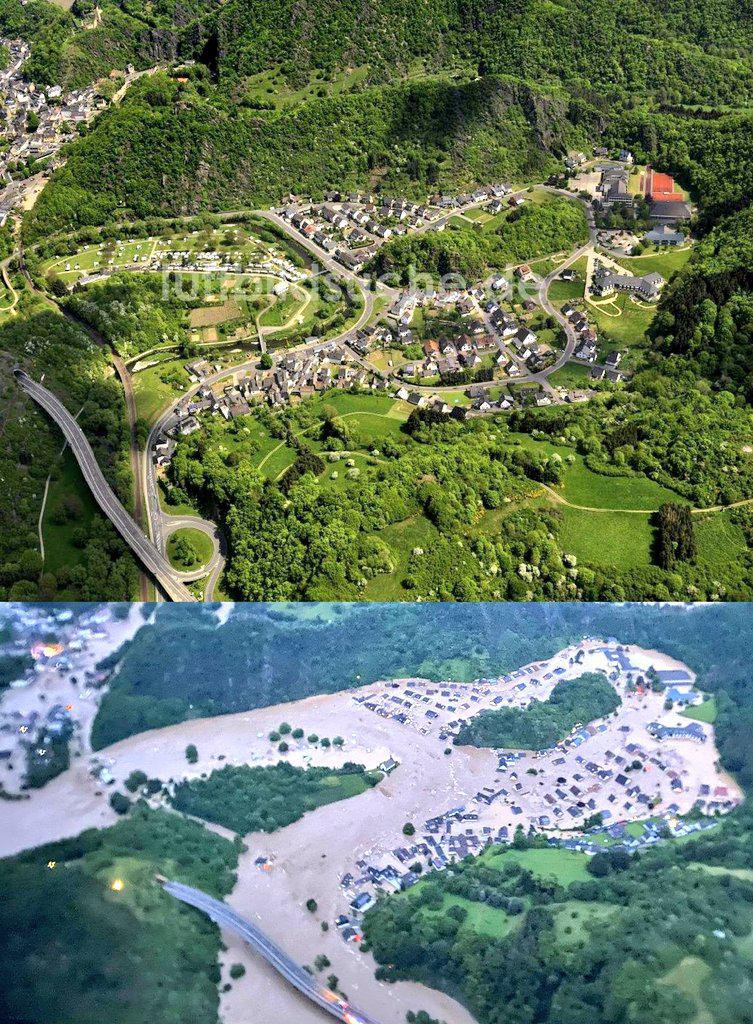
\includegraphics[width=\paperwidth,height=\paperheight]{cover_image.jpg}%
        }%
        \put(0,0){%
            \begin{tikzpicture}
                \fill[black, opacity=0.5] (0,12.3cm) rectangle (\paperwidth,22cm);
                % Near-opaque white band behind the bottom logo strip, so
                % the logos (usually designed for a light background) stay
                % legible regardless of image content underneath. Adjust
                % the y-values if the logos don't land inside this band.
                \fill[white, opacity=0.5] (0,0cm) rectangle (\paperwidth,3cm);
                \node[anchor=south west] at (3cm,0.65cm) {
\includegraphics[height=2cm]{tu_logo.png}};
                \node[anchor=south east] at (\paperwidth-3cm,0.9cm) {
\includegraphics[height=1.3cm]{deltares_logo.png}};
            \end{tikzpicture}%
        }%
    }
    \centering
    \vspace*{6cm}
    % Text is white, sitting on the dark scrim above -- if you widen/move
    % the scrim, keep the text colour white to match.
    {\color{white}
    {\Huge \bfseries Adapting a Graph Neural Network Surrogate\\
    for Fluvial Flood Simulation}\\[0.8cm]
    {\Large Application of mSWE-GNN to the Ahr Basin}\\[2cm]
    {\Large Margherita Marrocolo}\\[0.4cm]
    {\large MSc Environmental Engineering -- TU Delft}
    }

\end{titlepage}
 
%================================================================
% TITLE PAGE (details)
%================================================================
 
\begin{titlepage}
    \begin{center}
 
        \vspace{1.5cm}
 
        {\Large \textsc{Delft University of Technology}}\\[0.4cm]
        {\large Faculty of Civil Engineering and Geosciences}\\[0.2cm]
 
        \vspace{2cm}
        {\LARGE \bfseries Adapting a Graph Neural Network Surrogate
        for Fluvial Flood Simulation:\\ [0.7cm]
        Application of mSWE-GNN to the Ahr Basin}\\[0.4cm]
        \vspace{3cm}
 
        \begin{minipage}[t]{0.45\textwidth}
            \begin{flushleft}
                \textit{Author:}\\[0.2cm]
                {\large \textbf{Margherita Marrocolo}}\\
                Student Number: 6304966
            \end{flushleft}
        \end{minipage}
        \hfill
        \begin{minipage}[t]{0.45\textwidth}
            \begin{flushright}
                \textit{Project duration:}\\[0.2cm]
                March 2026 -- September 2026
            \end{flushright}
        \end{minipage}
 
        \vspace{2cm}
 
        \begin{minipage}{0.9\textwidth}
            \textit{Thesis committee:}\\[0.3cm]
            \begin{tabular}{@{}ll}
                Riccardo Taormina, & TU Delft, main supervisor \\
                Markus Hrachowitz, & TU Delft, auxiliary supervisor \\
                Roberto Bentivoglio, & TU Delft, advisor \\
                Albrecht Weerts, & Deltares, supervisor \\
            \end{tabular}
        \end{minipage}
 
        \vfill
 
        {\large MSc Thesis}\\[0.2cm]
        {\large Environmental Engineering, Water Management}\\[0.4cm]
        
        {\textit{Cover photo:} Stefan (Hellevoetsluis), 15 July 2021}
 
    \end{center}

      \begin{tikzpicture}
                \node[anchor=south west] at (3cm,0cm) {
\includegraphics[height=2cm]{tu_logo.png}};
                \node[anchor=south east] at (\paperwidth-3cm,0.2cm) {
\includegraphics[height=1.3cm]{deltares_logo.png}};
            \end{tikzpicture}

\end{titlepage}
 
%================================================================
% PAGE NUMBERING
%================================================================
\pagenumbering{roman}

%================================================================
% ABSTRACT
%================================================================

\chapter*{Abstract}
\addcontentsline{toc}{chapter}{Abstract}

Graph Neural Networks (GNNs) have recently emerged as computationally efficient
surrogates for physics-based flood models, with mSWE-GNN representing a significant
advance through its multi-scale, physics-informed message-passing architecture.
However, mSWE-GNN has so far only been validated on dike-breach scenarios, where
flooding originates from a localised structural failure; its applicability to riverine
(fluvial) flooding, driven by upstream discharge hydrographs, has remained untested.
This thesis adapts and evaluates mSWE-GNN for fluvial flood simulation, using the July
2021 Ahr River flood in Germany as a case study and SFINCS as the physics-based
reference solver.
 
Extending the model to fluvial forcing required architectural changes beyond a simple
boundary-condition update: the ghost-cell mechanism was generalised from a single
breach point to seven simultaneous tributary inflows, and training required a two-step
warm-start procedure, since a dry initial condition, standard for the model's original
dike-breach application, caused training to collapse to a degenerate all-dry
prediction. Hydraulic structures (levees, flow obstructions) were represented as an additional
edge feature on the finest mesh scale.
 
The best-performing configuration, trained on twenty SFINCS simulations, reached a
Critical Success Index of 0.853 (0.05~m threshold) on an event held out entirely from
training, a level of accuracy sufficient to support scenario-based analysis.
Performance improved consistently with training-data diversity, though complete
drainage of the catchment beyond the training horizon was never reliably learnt, and
structure representation generalised well for levees but poorly for flow obstructions, which is consistent with the small proportion of mesh edges affected by the structure. Contrary to
the model's original literature, the surrogate offered no consistent speed advantage
over SFINCS: it was slower on CPU and only modestly faster on GPU,likely reflecting the fact that SFINCS is already a computationally efficient, subgrid-corrected solver rather than showing a
failure of the adaptation.
 
These findings show that mSWE-GNN can be extended to riverine flooding, but not as a
drop-in application: the required adaptations are substantial, and the resulting
model's reliability for practical use varies by scenario type, training-data density,
and distance from the conditions seen during training.

\tableofcontents


%================================================================
% CHAPTER 1: INTRODUCTION
%================================================================


\chapter{Introduction}
\label{ch:introduction}
\pagenumbering{arabic}
\setcounter{page}{1}


\section{Motivation}
\label{sec:motivation}

\textit{Human history can be read as a continuous attempt to loosen the constraints imposed by nature.} As early as the eighteenth century, Turgot described the progress of the human mind as a process through which humanity gradually escapes the repetitive cycles governing the natural world \citep{turgot1750philosophical}. Yet, the ability to reshape our environment has come with consequences of its own. The same technological and economic development that has enabled societies to overcome many natural constraints has also intensified human pressure on natural systems.

Land-use change and anthropogenic climate change have altered the hydrological cycle, contributing to changes in the frequency and intensity of several classes of extreme events. The IPCC's Sixth Assessment Report finds that human influence has contributed to the intensification of heavy precipitation and other climate extremes, with implications for flood hazards \citep{ipcc2021ar6}. For flood risk, these changes can translate into higher extreme discharges, altered rainfall-runoff dynamics, and reduced natural buffering capacity. As flood hazards become increasingly dynamic and uncertain, water management therefore requires tools capable not only of representing how floods propagate through space and time, but also of evaluating how different interventions may modify their evolution.

This need extends beyond predicting the propagation of an individual flood event. Effective adaptation requires assessing how structural and nature-based measure perform under a range of hydrological conditions. Such what-if analyses can require the evaluation of many alternative scenarios, creating a growing demand for flood modelling approaches that are both physically credible and computationally efficient.


\section{Problem Statement}
\label{sec:statement}

Flood inundation modelling is fundamental to understanding and managing flood risk. Modelling approaches have evolved from simplified one-dimensional representations towards two-dimensional hydrodynamic models that resolve the spatial and temporal evolution of flood flows by numerically solving the Shallow Water Equations. Models such as Delft3D and SOBEK~2D can represent complex floodplain processes with high physical detail \citep{deltares2024delft3dsobek}, but this comes at a considerable computational cost. The burden becomes particularly relevant for large domains, fine resolutions, long simulations, and ensembles of scenarios, limiting applications such as real-time forecasting, uncertainty quantification, and probabilistic flood hazard assessment \citep{bentivoglio2022review,pianforini2024ensemble}. This has motivated the development of machine-learning-based surrogate models that aim to reproduce flood dynamics at substantially lower computational cost.

Early data-driven approaches largely relied on Convolutional Neural Networks (CNNs), which are well suited to regular grid-based representations but less naturally applicable to irregular geometries and unstructured hydraulic meshes \citep{bentivoglio2023swegnn,pianforini2024ensemble,taghizadeh2025hydrographnet}. Graph Neural Networks (GNNs) provide a more flexible alternative by representing the computational domain as a graph, with nodes and edges encoding spatial and topological relationships. This makes them naturally compatible with unstructured meshes and allows information to propagate according to the connectivity of the hydraulic domain \citep{bentivoglio2022review,bentivoglio2023swegnn,taghizadeh2025hydrographnet}. 

Despite these advances, the transferability of DL surrogates to different flood-generating mechanisms and boundary-condition configurations remains limited. Existing approaches to fluvial flooding generally focus on specific domains and forcing configurations, with limited evidence of generalisation to spatially distinct inflow locations within the same river system. In contrast, mSWE-GNN has demonstrated generalisation to unseen boundary conditions and boundary locations in its original dike-breach application (Bentivoglio et al., 2025), making it a natural candidate for extension to fluvial flooding. However, the model was originally developed for dike-breach scenarios, in which flooding originates from a localised breach, rather than from multiple upstream discharge hydrographs. This thesis therefore adapts and evaluates mSWE-GNN for fluvial flood modelling in the Ahr River basin, including the representation of multiple simultaneous inflows. Beyond assessing whether the adapted model can reproduce fluvial flood dynamics, the study investigates its potential for computationally efficient scenario-based analysis, including hypothetical hydraulic interventions.


\section{Research Objective}

\label{sec:objective}

The main research question, following naturally from the problem statement, is:

\begin{quote}
\emph{To what extent can the AI-based model mSWE-GNN be adapted to simulate riverine flooding beyond its original dike-breach application, while accelerating flood simulations and maintaining sufficient predictive accuracy for scenario-based flood analysis?}
\end{quote}


\section{Research Sub-Questions}

\label{sec:subquestions}

Achieving this objective requires answering the following five sub-questions:

\begin{itemize}
    \item[\textbf{SQ1}] What adaptations to the mSWE-GNN architecture are required to extend the model from dike-breach to fluvial flood modelling?

    \item[\textbf{SQ2}] How can hydraulic interventions, such as dikes, levees, and retention areas, be represented within the mSWE-GNN framework?

    \item[\textbf{SQ3}] How accurately can the adapted mSWE-GNN reproduce the spatio-temporal dynamics of fluvial flooding, and how does its computational performance compare with physics-based hydrodynamic modelling?

    \item[\textbf{SQ4}] How well does the adapted mSWE-GNN perform across flood scenarios with varying discharge conditions and magnitudes within the Ahr River catchment?

    \item[\textbf{SQ5}] How reliably can the surrogate model be used for what-if analyses in scenarios for which no direct observations are available?
\end{itemize}




%================================================================
% CHAPTER 2: THEORETICAL BACKGROUND
%================================================================
 
\chapter{Background}
\label{ch:background}
 
\section{Flood Inundation Modelling}
\label{sec:flood_modelling}
 
\subsection{Physics-Based Hydrodynamic Modelling}
\label{subsec:physics_based}

Water depth and flow velocity
evolve continuously in space and time as a flood wave propagates across a catchment, this makes flood inundation a spatio-temporal hydraulic process.
Traditional physics-based hydrodynamic models represent this by numerically solving the governing equations.
The dynamics
of shallow flows are commonly described by the two-dimensional
Shallow Water Equations (SWE), which express the conservation laws of mass and momentum under the
assumption that vertical accelerations are negligible relative to horizontal flow
processes \citep{vreugdenhil1994numerical}.
%\textcolor{blue}{note: add SWE equation? maybe not as not used afterwards}
Two-dimensional formulations of the SWE allow the model to represent spatial
variation of flow across the floodplain, rather than treating discharge as a single
value along a channel.

 
\subsection{Numerical solution of flood dynamics}
\label{subsec:num_solutions}
 
Solving the SWE over a real domain requires discretising space into a mesh and integrating the equations over each mesh element.
The Finite-Volume Method (FVM) is
the most common choice for hydrodynamic solvers, as it conserves mass and momentum
exactly across each discrete cell \citep{toro2001shock}
%,bentivoglio2023swegnn}
. In an FVM
formulation, the state of each computational cell is updated by exchanging fluxes with
its neighbouring cells: at every time step, each cell's water depth and discharge evolve
based only on the flow crossing its own boundaries. Information originating at one
location therefore propagates outward step by step, cell to cell, following the mesh's
connectivity, rather than being resolved globally in one operation.


\subsection{Computational limitations of physics-based models}
\label{subsec:limitations_physicbased}

The accuracy of a physics-based hydrodynamic model is tied to its spatial resolution,
but resolution and computational cost are not independent. Explicit numerical schemes
must satisfy a stability condition: the Courant--Friedrichs--Lewy (CFL) condition,
that limits the largest stable time step to a value set by the grid spacing and the
wave celerity of the flow. Refining the spatial resolution therefore has a compounding\textcolor{blue}{note:wouldn't use this term}
effect: it increases the number of cells to be solved and forces a smaller time
step, so that computational cost grows faster than linearly with resolution
\citep{toro2001shock,bates2010simple}. For large domains, fine
resolutions, long simulation periods, or ensembles of scenarios, this cost becomes
prohibitive for the kind of repeated, rapid evaluation that operational forecasting and
scenario-based analysis require (Section~\ref{sec:motivation}). This
computational bottleneck is the central motivation for the data-driven surrogate
modelling approaches reviewed in Section~\ref{sec:surrogates}.

\section{SFINCS as a Reference Flood Model}
\label{sec:sfincs_reference}

SFINCS \citep{leijnse2021sfincs} is used in this study as the reference hydrodynamic
model against which the surrogate model is trained and evaluated. SFINCS is adopted here
as a physically based benchmark, one that is considerably cheaper to run than a
full-resolution hydrodynamic model, against which the ability of the GNN surrogate to
reproduce flood dynamics can be assessed.
 
\subsection{SFINCS approach and simplifications}
\label{subsec:sfincs_simplifications}
 
SFINCS achieves its computational efficiency through two main simplifications relative
to a full SWE solver \citep{vanormondt2025sfincs}. First, it adopts a local inertial
approximation, which drops the advective acceleration terms from the momentum equation.
This reduces the cost of each time step and relaxes the CFL constraint described in
Section~\ref{subsec:limitations_physicbased}, at the cost of some accuracy in settings
where advective effects are significant \citep{bates2010simple}. Second, it applies a
subgrid correction: high-resolution terrain and roughness statistics are pre-computed as
lookup tables, so that at each time step the model recovers hydraulically consistent
depth and roughness values on a coarse computational grid. Together, these two
simplifications allow SFINCS to run on grids one to two orders of magnitude coarser than
the underlying terrain model while retaining much of the hydraulic fidelity of a
full-resolution solve \citep{vanormondt2025sfincs}.
 
\subsection{FINCS for fluvial flood simulation}
\label{subsec:sfincs_fluvialflood}
 
SFINCS supports several forcing and boundary condition types.
Meteorological forcing, including spatially distributed rainfall, can be prescribed
directly over the domain. In fluvial settings, the primary forcing is instead one or
more time-varying discharge hydrographs imposed at upstream source points, which is the
forcing type adopted throughout this thesis (Section~\ref{subsec:forcing_data}). At the
downstream end of a domain, a water-level boundary can represent backwater effects from
a receiving water body, or an outflow condition can be imposed to let water leave the
domain freely. SFINCS can additionally represent hydraulic structures such as levees,
thin dams, and weirs, which is what makes it suitable for generating the structure
scenarios used in this thesis' what-if analysis
(Section~\ref{sec:hydraulic_structures_method}). Beyond forcing, SFINCS produces
spatially distributed hydraulic fields (water level and velocity) across the
domain, as well as time series at user-defined observation points, both of which serve
as reference data for training and evaluating the surrogate model. 
%The specific
%procedure for extracting these fields and converting them into GNN training data is
%described in Chapter~\ref{ch:methodology}.
 
\section{Deep Learning Surrogates for Flood Modelling}
\label{sec:surrogates}
The computational limitations discussed in Section~\ref{subsec:limitations_physicbased}
have motivated a growing body of work on data-driven surrogate models for flood
inundation.
Flood-surrogate studies differ not only in model architecture, but also in the type of flooding, prediction task, and representation of hydraulic forcing. Applications include pluvial flooding driven by spatially distributed rainfall, fluvial flooding driven by river discharge, coastal flooding driven primarily by water-level or wave forcing, and dike-breach flooding originating from a localised structural failure. Surrogates may further target either point-based predictions, such as water level at selected locations, or spatial predictions of hydraulic variables across the full domain. For spatial models, forcing can be represented globally across the domain or explicitly associated with specific boundary locations, with one or multiple boundary conditions acting simultaneously. 
This section traces how that field has evolved: from early machine-learning
approaches, to
convolutional architectures, to the
graph-based architectures.
 
\subsection{From Conventional ML to Spatial Deep Learning}
\label{subsec:conventional_ml}
 
Early machine-learning surrogates for flood inundation typically learned a mapping from
a small number of scalar forcing or scenario parameters to a scalar or low-dimensional
flood characteristic, rather than explicitly learning the full spatio-temporal
evolution of the flood. \citet{liu2015svr} trained a vector regression model to
emulate the water depths and velocities of a fine-grid hydrodynamic model at a limited
set of target locations, learning a direct mapping from model inputs to those output
locations rather than to a full inundation map. \citet{bermudez2019lssvm} extended this
kind of approach spatially, using a least-squares support vector machine to estimate the
spatial distribution of maximum water depth and velocity in a coastal urban catchment,
with discharge in three streams and tide levels as predictor variables.
\citet{berkhahn2019ensemble} used an ensemble of neural networks to predict, in
real time, the maximum water levels reached during a flash-flood event driven by
spatially uniform rainfall. These studies established that flood characteristics could be predicted directly from forcing data at a fraction of the cost of a hydrodynamic simulation. However, they primarily targeted either selected locations or spatial summary quantities, rather than the spatially and temporally resolved hydraulic state across the full domain.
 
Producing a full flood map instead requires a model capable of learning spatial
structure directly, which motivated the shift toward spatial deep learning.

\subsection{CNN-based flood surrogates}
\label{subsec:cnn}

CNNs became an attractive choice for flood surrogate modelling for several reasons: they
take spatially structured, gridded inputs and outputs (matching how terrain, land use,
and flood maps are typically represented as rasters); their local receptive fields and
weight sharing make them substantially more parameter-efficient than a fully-connected
network over the same domain; and, once trained, they can generate a complete spatial
flood map in a single forward pass rather than a sequence of point predictions
. Kabir et al. (2020) applied a CNN to fluvial flooding, using outputs from the 2D hydraulic model LISFLOOD-FP to predict water depths across more than half a million grid cells directly from a sequence of upstream discharge inputs. Guo et al. (2021) instead framed pluvial flood prediction as an image-to-image translation problem, predicting maximum water depth and reporting inference times of around 0.5\% of the corresponding hydrodynamic simulation. Løwe et al. (2021) similarly developed the CNN-based U-FLOOD architecture for urban pluvial flooding, predicting water depth directly from terrain and rainfall inputs.

 
These successes, however, exposed a shared, fundamental limitation: CNNs assume input
and output data lie on a regular, Euclidean grid. This assumption is convenient for
rasterised terrain and rainfall data, but it does not hold for the unstructured,
irregular meshes commonly used by hydrodynamic solvers to resolve complex or
variable-resolution terrain, nor does it naturally accommodate domains of different size
and shape without retraining or extensive pre-processing
\citep{bentivoglio2023swegnn,bentivoglio2022review}. This limitation, is what motivated the shift toward graph-based architectures, discussed
next.
 
\subsection{GNNs for flood modelling}
\label{subsec:gnn}
 
Graph Neural Networks (GNNs) represent the computational domain as a graph
$\mathcal{G} = (\mathcal{V}, \mathcal{E})$ rather than a regular grid, with nodes
$\mathcal{V}$ and edges $\mathcal{E}$ free to follow the connectivity of an arbitrary,
irregular mesh \citep{bronstein2021geometric}. This directly addresses the CNN
limitation discussed above: a GNN can operate on the same unstructured mesh a
hydrodynamic solver uses, without requiring the domain to be rasterised onto a regular
grid. A further property relevant to flood modelling is permutation equivariance: a
GNN's prediction at a given node depends only on that node's local neighbourhood, not on
how nodes happen to be indexed or ordered \citep{bronstein2021geometric}.
This makes GNN
architectures naturally robust to irregular mesh geometry and, in principle, transferable
across different domains and topographies without retraining, an advantage that has been
demonstrated for physical simulation tasks more broadly
\citep{sanchezgonzalez2020learning}.
 
Bentivoglio et al. (2023) introduced SWE-GNN for spatial prediction of dike-breach inundation, with the breach represented as a localised boundary forcing within the graph. It is the first GNN surrogate explicitly designed to mirror the structure of a finite-volume SWE solver (Section~\ref{subsec:num_solutions}). The computational mesh is mapped directly to a graph, while the local message-passing mechanism is conceptually analogous to the flux exchange between neighbouring finite-volume cells, providing a natural graph-based representation of flood propagation. SWE-GNN achieved substantial speed-ups over a full-resolution hydrodynamic reference while maintaining acceptable spatial accuracy on unseen topographies.

 
Subsequent work has extended hydraulic GNNs along several directions.
\citet{kazadi2024floodgnngru} proposed FloodGNN-GRU, which combines a GNN with a Gated
Recurrent Unit to capture the temporal evolution of pluvial flooding  using rotation-equivariant operations so that the model's response does not depend on the arbitrary orientation of the
input mesh. \citet{taghizadeh2025hydrographnet} introduced HydroGraphNet, a physics-informed GNN that enforces mass conservation through the loss function and produces spatial predictions of flood dynamics across a combined urban-rural domain. The model considers both rainfall and upstream river discharge; however, the fluvial forcing is represented as a single global discharge feature shared across all graph nodes. It therefore does not explicitly represent multiple, spatially localised inflow boundary conditions within the river system.

Building on these developments, Bentivoglio et al. (2025) introduced mSWE-GNN, a multi-scale extension of SWE-GNN that demonstrated generalisation across different mesh resolutions, topographies, boundary conditions, and boundary-condition locations. However, these experiments remained focused on dike-breach flooding, where each scenario is driven by a localised breach rather than by multiple simultaneous inflows within a fluvial network. This demonstrated transferability makes mSWE-GNN particularly relevant to the problem addressed in this thesis. The model architecture is described in Section~\ref{sec:mswegnn}.

 

%================================================================
% CHAPTER 3: METHODOLOGY
%================================================================
 
\chapter{Methodology}
\label{ch:methodology}
 
This chapter describes the reproducible workflow used to adapt mSWE-GNN to riverine
flooding: producing a physics-based reference simulation, converting it into GNN
training data, extending the architecture and boundary condition mechanism to fluvial
forcing, representing hydraulic structures, and defining the metrics used to evaluate
the surrogate.
Their application to the
Ahr basin is presented in Chapter~\ref{ch:case_study}
 
\begin{figure}[H]
    \centering
    \resizebox{0.32\textwidth}{!}{%
    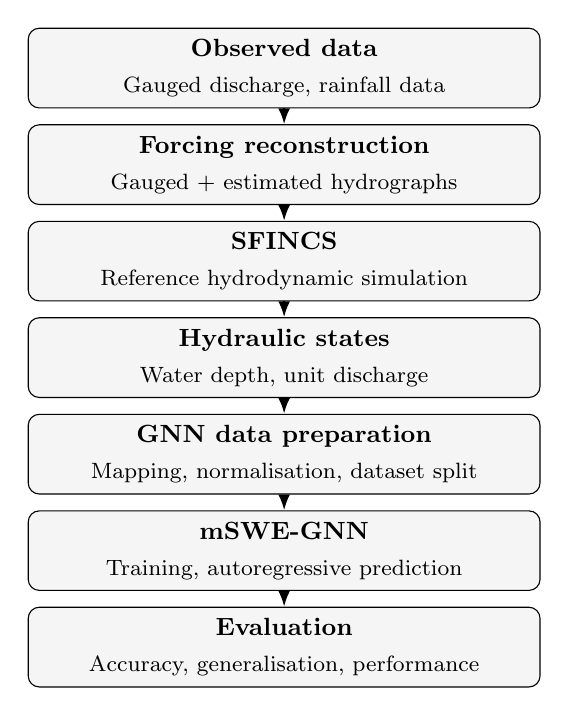
\begin{tikzpicture}[
        node distance=0.2cm and 0cm,
        box/.style={rectangle, draw, rounded corners, fill=gray!8,
            minimum width=6.5cm, minimum height=1cm, align=center,
            font=\small, inner sep=4pt},
        arr/.style={-{Latex[length=2mm]}, thick}
    ]
        \node[box] (n1) {\textbf{Observed data}\\[2pt]
            \footnotesize Gauged discharge, rainfall data};
        \node[box, below=of n1] (n2) {\textbf{Forcing reconstruction}\\[2pt]
            \footnotesize Gauged + estimated hydrographs};
        \node[box, below=of n2] (n3) {\textbf{SFINCS}\\[2pt]
            \footnotesize Reference hydrodynamic simulation};
        \node[box, below=of n3] (n4) {\textbf{Hydraulic states}\\[2pt]
            \footnotesize Water depth, unit discharge};
        \node[box, below=of n4] (n5) {\textbf{GNN data preparation}\\[2pt]
            \footnotesize Mapping, normalisation, dataset split};
        \node[box, below=of n5] (n6) {\textbf{mSWE-GNN}\\[2pt]
            \footnotesize Training, autoregressive prediction};
        \node[box, below=of n6] (n7) {\textbf{Evaluation}\\[2pt]
            \footnotesize Accuracy, generalisation, performance};

        \draw[arr] (n1) -- (n2);
        \draw[arr] (n2) -- (n3);
        \draw[arr] (n3) -- (n4);
        \draw[arr] (n4) -- (n5);
        \draw[arr] (n5) -- (n6);
        \draw[arr] (n6) -- (n7);
    \end{tikzpicture}%
    }
    \caption{Overview of the methodology workflow.}
    \label{fig:methodology_workflow}
\end{figure}
 
\section{Data Curation}
\label{sec:data_curation}
 
Training and validation data for the surrogate model are generated using SFINCS \citealp{leijnse2021sfincs} as the reference hydrodynamic model (Section~\ref{sec:sfincs}). Observed and reconstructed discharge hydrographs are first used to force SFINCS simulations, which generate the spatially and temporally distributed hydraulic states used as reference data. These outputs are subsequently mapped to the GNN representation and processed into training, validation, and test datasets, from which mSWE-GNN learns to reproduce the simulated flood dynamics. The following sections describe each stage of this workflow.

 
%\subsection{Input Data Preparation}
%\label{subsec:input_data}
 
%A DEM is reprojected into the local UTM zone and, serves both to define bed elevation at the
%computational grid level and to derive subgrid lookup tables. The model domain polygon
%is derived from catchment-boundary data
%(e.g. HydroSHEDS, Lehner et al., 2008)
%and postprocessed in a GIS environment.
 
%When discharge hydrographs are used as forcing, the domain polygon must be modified so
%that each inflow source point lies exactly on the catchment boundary. %While SFINCS can
%accept source points anywhere within the domain, placing them on the boundary is
%required for compatibility with the mSWE-GNN ghost cell mechanism, which represents
%inflow locations as boundary nodes at the domain perimeter (Section~\ref{sec:model_adaptation}).
%Source points are snapped to the nearest point on the boundary polygon. At the
%downstream end, a fixed water depth of 0~m is imposed at the outflow boundary to
%let water leave the domain freely.
\textcolor{purple}{maybe add in teh experiments part}

\subsection{Forcing Data}
\label{subsec:forcing_data}
 
Discharge hydrographs are adopted as the primary fluvial forcing type, for two reasons. First, discharge is the dominant driver of fluvial flooding: most hydrodynamic flood models are primarily driven by an upstream discharge boundary condition (unless pluvial-fluvial dynamics are of interest) \citep{saksena2019flood}. Second, the original mSWE-GNN architecture was designed around discharge-hydrograph boundary conditions imposed via ghost cells, and extending it to accept spatially distributed rainfall would require substantial modifications to both the input encoding and the boundary condition mechanism \citep{bentivoglio2025mswegnn}.
 
 
\subsection{Estimating Discharge at Ungauged Tributaries}
\label{subsec:ungauged}
 
In a river catchment, not every sub-catchment is instrumented: a downstream reference gauge and some, but typically not all, of the tributaries draining into the reach upstream of it may carry a discharge record, while the remaining, ungauged sub-catchments contribute flow with no direct observation. Before these locations can be used as ghost-cell forcing points (Section~\ref{subsec:model_adaptation_detail}), their discharge must be estimated.

This estimation matters for two reasons. First, estimating the discharge of ungauged tributaries requires assumptions about rainfall-runoff response and routing, introducing uncertainty into the boundary conditions supplied to the hydrodynamic model. This uncertainty subsequently propagates into the simulated hydraulic states used as training and evaluation data for the GNN. Second, the choice of reconstruction method is itself a modelling decision that may influence the resulting flood dynamics, particularly near ungauged inflow locations. Three alternative reconstruction methods are considered, differing in how the ungauged contribution is distributed and routed. One method is adopted as the primary for training and testing throughout this thesis, while the full set is later used to test whether the model's behaviour is sensitive to this particular modelling choice (Section~\ref{sec:physics_sensitivity_method}).
The primary method is selected because it introduces the fewest additional assumptions about the total flood volume supplied to the training data.

Let $Q_\text{outlet}(t)$ denote the discharge observed at the downstream reference
gauge, and $Q_j(t)$, $j \in \text{gauged}$, the discharge observed at each gauged
tributary. The residual

\begin{equation}
    Q_\text{res}(t) = Q_\text{outlet}(t) - \sum_{j \in \text{gauged}} Q_j(t)
    \label{eq:residual}
\end{equation}

represents the combined contribution of every ungauged sub-catchment, and must be
apportioned among the $i$ ungauged points before it can be used as forcing. Methods 1
and 2 below both distribute this residual, differing in how they weight and time it
across points; Method 3 instead estimates each ungauged point's discharge
independently, without reference to the outlet record at all.

\paragraph{Method 1: Area-Weighted Residual.}
This method distributes $Q_\text{res}(t)$ among the ungauged points in proportion to
catchment area, applying a single advance shift $\Delta t$ common to every point,
obtained from the cross-correlation lag between the gauged tributary sum and the
outlet record:

\begin{equation}
    Q_i(t) = \frac{A_i}{\sum_k A_k} \cdot Q_\text{res}(t - \Delta t)
    \label{eq:method1}
\end{equation}

where $A_i$ [km$^2$] is the catchment area of ungauged point $i$. By construction, this
method closes the mass balance at the outlet exactly. It rests on two simplifying
assumptions: uniform specific discharge across sub-basins, ignoring differences in
rainfall intensity, soil moisture, and land use between them; and a single uniform
routing lag, which does not account for ungauged points lying at different distances
from the outlet.

\paragraph{Method 2: Rainfall-Weighted Residual with Kirpich Routing Lag.}
This method also distributes $Q_\text{res}(t)$, but weights each point by catchment
area times mean areal rainfall intensity rather than area alone, which is physically
more consistent as it accounts for spatial variability in rainfall input across the
catchment \citep{beven2012rainfall}, and assigns each point its own routing lag
$\Delta t_i$ rather than a single shared value:

\begin{equation}
    w_i(t) = \frac{A_i \cdot R_i(t)}{\sum_k A_k \cdot R_k(t)}, \qquad
    Q_i(t + \Delta t_i) = w_i(t) \cdot Q_\text{res}(t)
    \label{eq:method2}
\end{equation}

where $R_i$ [mm/h] is catchment-averaged rainfall intensity. Each $\Delta t_i$ [h] is
estimated with the \citet{kirpich1940time} formula, applied along the channel network
from each tributary confluence to the outlet:

\begin{equation}
    \Delta t_i = 0.0663 \left(\frac{L_i}{\sqrt{S_i}}\right)^{0.77} \quad \text{[h]}
    \label{eq:kirpich}
\end{equation}

where $L_i$ [km] is the channel length from the tributary confluence to the outlet and
$S_i$ [m/m] is the average channel slope.

\paragraph{Method 3: SCS-CN Rainfall-Runoff with Triangular Unit Hydrograph.}
This method estimates discharge at each ungauged
point independently of the downstream observation entirely. Excess rainfall $Q_e$
[mm] is derived from cumulative rainfall $P$ [mm] using the SCS Curve Number method
\citep{usdanrcs2004}:

\begin{equation}
    S = \frac{25400}{CN} - 254 \quad \text{[mm]}, \qquad
    I_a = 0.2\,S, \qquad
    Q_e = \frac{(P - I_a)^2}{P + 0.8\,S}
    \label{eq:scscn}
\end{equation}

where $S$ [mm] is the potential maximum retention, $I_a$ [mm] is the initial
abstraction, and $CN$ is the curve number, which depends on land use, soil type, and
antecedent moisture condition (AMC). The time to peak $T_p$ [h] is estimated with the
\citet{giandotti1934previsione} formula:

\begin{equation}
    T_p = \frac{4\sqrt{A} + 1.5\,L}{0.8\,\sqrt{\Delta H}} \quad \text{[h]}
    \label{eq:giandotti}
\end{equation}

where $A$ [km$^2$] is the subcatchment area, $L$ [km] is the longest flow path, and
$\Delta H$ [m] is the difference between mean basin elevation and outlet elevation. A
triangular synthetic unit hydrograph \citep{usdanrcs2007,chow1988applied} is then
convolved with the incremental excess rainfall to produce the discharge hydrograph at
each source point:

\begin{equation}
    q_p = \frac{0.208\,A}{T_p}, \quad T_b = 2.67\,T_p, \qquad
    Q(t) = \sum_\tau \Delta Q_e(\tau) \cdot UH(t-\tau)
    \label{eq:uh}
\end{equation}

where $q_p$ [m$^3$/s/mm] is the unit peak discharge, $T_b$ [h] is the base time of the
triangular hydrograph, $\Delta Q_e(\tau)$ [mm] is the incremental excess rainfall at
time $\tau$, and $UH(t-\tau)$ is the unit hydrograph ordinate.
 
%\subsection{Grid and Subgrid Setup}
%\label{subsec:grid_subgrid}
 
%The SFINCS model is discretised on a regular Cartesian grid, with subgrid lookup
%tables derived from a high-resolution DEM at a finer subgrid resolution
%(Section~\ref{subsec:input_data}). The subgrid approach \citep{casulli2009wetting} allows the
%model to capture strong local topographic variability without requiring the full
%computational cost of a high-resolution hydrodynamic grid.
 
\subsection{Validation of the SFINCS Reference Simulation}
\label{subsec:sfincs_validation}
 
Before being used to generate GNN training data, the SFINCS reference simulation is
validated in two ways: against observed water depth at gauge stations, and against an
independent, observation-based flood-extent product. The
comparison is made between the simulated \emph{maximum} water extent and the mapped
flood-affected area. Both layers are rasterised to a common grid and, at a chosen
water-depth threshold, each pixel is classified as true positive (TP, flooded in both),
false positive (FP, flooded in the simulation only), or false negative (FN, flooded in
the reference product only), from which the Critical Success Index (CSI,
Section~\ref{sec:benchmarking}) is computed.
\textcolor{purple}{maybe completely move to case study as Roberto mentioned?}
 
\section{From SFINCS Simulations to GNN Training Data}
\label{sec:dataset_generation}
 
\subsection{Extracting Hydraulic Fields}
\label{subsec:sfincs_to_graph}
 
mSWE-GNN was originally developed for D-Hydro
outputs \citep{bentivoglio2025mswegnn}; adapting it to SFINCS requires converting terrain
and domain files to compatible formats and extracting hydraulic fields from the SFINCS
map-output structure. These are pre-processing changes that do not affect the model
architecture.
 
Water depth is computed as:
 
\begin{equation}
    WD = \max(z_s - z_b,\ 0)
    \label{eq:waterdepth}
\end{equation}
 
where $z_s$ [m] is the water surface elevation and $z_b$ [m] is the bed elevation.
Negative values, which can arise from numerical residuals in dry cells, are clamped to
zero. Velocity components $(u, v)$ [m/s] are also extracted and stored as dynamic
features. Fill values are masked before further processing.
 
The GNN mesh at the finest scale corresponds directly to the active SFINCS grid cells, so hydraulic outputs can be mapped directly to the corresponding interior graph nodes. The extracted data further include the time-varying boundary conditions required by the GNN, represented by water surface elevation and unit discharge at each boundary location. The complete set of quantities provided to the model is listed in Appendix~\ref{app:sim_data}.
 
\subsection{Feature Normalisation}
\label{subsec:normalisation}

Normalisation is applied only to the static node and edge features (DEM
elevation, cell area, and edge length) fitted on the training set only, to
prevent data leakage from validation/test simulations into training statistics
\citep{sasse2023leakage}. DEM values are shifted to a zero minimum to preserve
relative elevation differences. Cell area and edge length are standardised to
zero mean and unit variance separately at each of the $K$ mesh scales, since
these quantities grow systematically with resolution:

\begin{equation}
    \tilde{f}_k = \frac{f_k - \mu_k}{\sigma_k}, \quad k = 1, \dots, K
    \label{eq:scale_norm}
\end{equation}

where $\mu_k$ and $\sigma_k$ are the mean and standard deviation computed over the
training set at scale $k$. This prevents coarser-scale features from dominating due
to their larger absolute cell areas and edge lengths.
 
\subsection{Dataset Split}
\label{subsec:temporal_resolution}

The distinction between training, validation, and test is not one of data source but
of evaluation: training loss is computed over short, curriculum-limited rollout
windows (Section~\ref{subsec:training_validation}), whereas validation and test metrics are
computed over a single continuous autoregressive rollout spanning the full event.
When multiple simulations are used for training, the split is instead made at the
level of whole simulations: one or more simulations are held out entirely from
training and used for validation (to drive early stopping) and testing, so that
reported test metrics reflect a configuration never seen during training..

\section{The mSWE-GNN Framework}
\label{sec:mswe_gnn}

The model is asked to predict how water depth (and unit discharge) evolves through
time and space over the course of a flood event, given: (i) static properties of the
terrain that do not change during the event; and (ii) the time-varying boundary
forcing at the domain's inflow points. Water depth at every cell, at every time step,
is what ultimately determines flood extent, depth, and timing, the quantities needed
for flood risk analysis.
 
This field is produced autoregressively: rather than predicting the entire event in
one shot, the model advances the simulation one time step at a time, using its own
most recent predictions (over a short window of $p$ previous steps) as part of the
input for the next step.
 
mSWE-GNN \citep{bentivoglio2025mswegnn} follows an encoder-processor-decoder structure.
Moreover, it is designed to handle larger and more complex domains where a single
graph resolution is insufficient.
 
\subsection{Multi-Scale Mesh and Graph Construction}
\label{subsec:multiscale_mesh}

The model operates on a set of $M$ meshes of progressively coarser resolution. Each
scale is meshed as a frontal-Delaunay triangulation of the same
domain boundary polygon, at that scale's own uniform target element size. The barycentres of mesh cells become graph nodes,
and shared faces between cells become edges. Nodes across scales are connected by
directed inter-scale edges: if a fine mesh cell's centre falls within a coarse mesh
cell, a directed edge connects the two nodes \citep{bentivoglio2025mswegnn}.
 
\textcolor{blue}{note: add picture representing this mapping between scales 
%This connectivity is described by adjacency matrices $\mathbf{A}^m$ at each
%scale $m$ and prolongation matrices $\mathbf{P}^{m \rightarrow n}$ connecting adjacent
%scales.
}
 
\subsection{Encoder}
\label{subsec:encoder}
 
Three separate three-layer MLPs encode the raw input features into a common latent
space of dimension $G$. The inputs are:
 
\textbf{Static node features} $\mathbf{x}_{s,i} = (a_i, e_i, m_i)$, where $a_i$ is the cell
area [m$^2$], $e_i$ is the surface elevation [m], and $m_i$ is the Manning roughness
coefficient [s/m$^{1/3}$]. These are time-invariant and characterise the hydraulic
environment independently of the flow state. The static encoder is applied at all
scales, since physical quantities should have similar embeddings regardless of
resolution.
 
\textbf{Dynamic node features} $\mathbf{x}_{d,i} = (h_i^t, |q|_i^t)_{t-p:t}$, where $h_i^t$
[m] is the water depth and $|q|_i^t$ [m$^2$/s] is the unit discharge magnitude over
the $p$ most recent time steps. The dynamic encoder is applied only at the finest scale.
 
\textbf{Edge features} $\boldsymbol{\epsilon}_{ij} = (l_{ij})$, where $l_{ij}$ is the length of
the dual edge between nodes $i$ and $j$ [m]. The edge encoder is applied at all scales.
 
The encoded representations $\mathbf{H}_s$, $\mathbf{H}_d$, and $\boldsymbol{\mathcal{E}}'$
are higher-dimensional versions of the original inputs that are more expressive and form
the input to the processor \citep{bentivoglio2025mswegnn}.
 
\subsection{Processor}
\label{subsec:processor}
 
The processor propagates the encoded inputs through the multi-scale graph in a U-shaped
fashion, with a downsampling branch from fine to coarse and an upsampling branch from
coarse to fine \citep{bentivoglio2025mswegnn,gao2019graphunets}.
\textcolor{blue}{add picture of the U-shaped architecture}
 
In the downsampling branch, $L$ GNN layers are applied at the finest scale
$\mathcal{M}_1$. Each GNN layer computes inter-node messages as:
 
\begin{equation}
    \mathbf{s}_{ij}^{(\ell+1)} = \psi\!\left(\mathbf{h}_{s,i},\, \mathbf{h}_{s,j},\,
    \mathbf{h}_{d,i}^{(\ell)},\, \mathbf{h}_{d,j}^{(\ell)},\,
    \boldsymbol{\epsilon}_{ij}'\right) \odot
    \left(\mathbf{h}_{d,j}^{(\ell)} - \mathbf{h}_{d,i}^{(\ell)}\right)
    \label{eq:message}
\end{equation}
 
where $\psi(\cdot): \mathbb{R}^{5G} \rightarrow \mathbb{R}^G$ is a multi-layer
perceptron and $\odot$ is the Hadamard (element-wise) product. The gradient term
$(\mathbf{h}_{d,j}^{(\ell)} - \mathbf{h}_{d,i}^{(\ell)})$ acts as a physical
constraint ensuring that water propagates only from nodes that already carry water,
suppressing unphysical backflow \citep{bentivoglio2025mswegnn}. Node states are updated by:
 
\begin{equation}
    \mathbf{h}_{d,i}^{(\ell+1)} = \mathbf{h}_{d,i}^{(\ell)} +
    \sum_{j \in \mathcal{N}_i} \mathbf{s}_{ij}^{(\ell+1)} \mathbf{W}^{(\ell+1)}
    \label{eq:node_update}
\end{equation}
 
where $\mathbf{W}^{(\ell+1)} \in \mathbb{R}^{G \times G}$ are learnable parameter
matrices and $\mathcal{N}_i$ is the set of neighbours of node $i$. After the GNN layers
at scale $\mathcal{M}_1$, a mean pooling operator maps node features to the next coarser
scale $\mathcal{M}_2$. This is repeated until the coarsest scale is reached.
 
In the upsampling branch, a learnable MLP-based operator maps features from
each coarser scale back to the next finer scale. Skip connections then sum the output of
the downsampling GNNs at scale $\mathcal{M}_m$ with the upsampled features arriving
from $\mathcal{M}_{m+1}$, after which another set of $L$ GNN layers is applied. This
continues until the finest scale is restored. GNN layers, downsampling, and upsampling
operators are not shared across scales; each acts independently at its given scale.
 
The multi-scale design allows GNN layers at each scale to cover different spatial ranges.
Coarser scales capture fast, long-range channel dynamics efficiently, while fine scales
preserve local floodplain detail. This also reduces the number of GNN layers needed at
the finest scale, since one layer at a coarse scale covers the equivalent of several
layers at the finest scale \citep{bentivoglio2025mswegnn}.
 
\subsection{Decoder}
\label{subsec:decoder}
 
The decoder estimates the predicted hydraulic variables at time $t+1$ as a combination
of the processor output at the finest scale and the $p$ previous input time steps:
 
\begin{equation}
    \hat{\mathbf{u}}_i^{t+1} = \varphi\!\left(\mathbf{h}_{d,i}\right) +
    \sum_{\tau=1}^{p} w_\tau \, \mathbf{x}_{d,i}^{t-\tau+1}
    \label{eq:decoder}
\end{equation}
 
where $\varphi(\cdot)$ is a three-layer MLP that decodes the processor embedding
$\mathbf{h}_{d,i}$, and $w_\tau$ are learnable weights that act as a 1D convolutional
layer along the temporal axis, weighing the contribution of each past time step. A ReLU
activation at the output ensures non-negative values for water depth and unit discharge
\citep{bentivoglio2025mswegnn}.
 
\subsection{Boundary Conditions via Ghost Nodes}
\label{subsec:ghost_nodes}
 
Boundary conditions are handled via ghost cells, as is common in numerical methods
\citep{leveque2002finite}. Ghost cells are artificial nodes added at the domain boundary that are
not part of the physical domain but act as a link to external forcing. For inflow
conditions, directed edges connect ghost cells towards the real mesh; for outflow, edges
point in the opposite direction. At each autoregressive time step the state of the ghost
cells is overwritten with the prescribed boundary value, either a water level or a unit
discharge \citep{bentivoglio2025mswegnn}.
 
 
\subsection{Training Loss and Curriculum Learning}
\label{subsec:training_validation}
 
Training uses a multi-step-ahead forecasting loss to prevent error accumulation during
autoregressive rollout \citep{bentivoglio2025mswegnn}:
 
\begin{equation}
    \mathcal{L}_f = \frac{1}{HO} \sum_{\tau=1}^{H} \sum_{o=1}^{O} \gamma_o
    \left\| \hat{\mathbf{u}}_o^{t+\tau} - \mathbf{u}_o^{t+\tau} \right\|_2^2
    \label{eq:forecast_loss}
\end{equation}

where $H$ is the forecast horizon, the number of future time steps included in the
training rollout, and $O$ is the number of predicted output variables per node (water
depth and unit discharge magnitude). $\hat{\mathbf{u}}_o^{t+\tau}$ and
$\mathbf{u}_o^{t+\tau}$ are the predicted and ground-truth values of output variable
$o$ across all mesh nodes at forecast step $t+\tau$, respectively, and
$\|\cdot\|_2^2$ is the squared $\ell_2$ norm, summing the squared error over every
node in the mesh. $\gamma_o$ is a weighting coefficient applied to output variable
$o$, allowing depth and discharge errors to be balanced against each other in the
combined loss. In every reported configuration $\gamma_o$ is fixed at
$\gamma_\text{depth}=1$ for water depth and $\gamma_\text{discharge}=7$ for unit
discharge magnitude, so the discharge term contributes seven times as much as the
depth term to $\mathcal{L}_f$, even though only water-depth accuracy is reported as
a validation and test metric (Section~\ref{sec:benchmarking}).

A mass conservation penalty can be added to discourage volume errors:
 
\begin{equation}
    \mathcal{L}_c = \left( \sum_{i=1}^{N} a_i \, \Delta \hat{h}_i - Q \Delta t \right)^2
    \label{eq:mass_loss}
\end{equation}
 
giving the combined loss $\mathcal{L} = \mathcal{L}_f + \lambda \mathcal{L}_c$, where
$\lambda$ balances accuracy against physical consistency
\citep{bentivoglio2025mswegnn,taghizadeh2025hydrographnet}.

The model uses $p$ previous timesteps as dynamic input at each prediction step; the
value is adopted from \citet{bentivoglio2025mswegnn}. The rollout horizon $H$ over which $\mathcal{L}_f$
(Eq.~\ref{eq:forecast_loss}) is computed is increased gradually from 1 to its final
value over training epochs using curriculum learning, which helps avoid instability
from backpropagating through long rollouts from the start of training
\citep{bengio2009curriculum}; the final value trades off training time (which grows
with rollout length) against accuracy and training stability.

Beyond the base forecast and mass-conservation terms, three modifications to the
loss formulation are considered. 

First, the application of a shallow-water weight
$w$ to wet cells within a shallow depth range $0 < \text{WD} \le \text{WD}_\text{max}$,
multiplying the corresponding term in $\mathcal{L}_f$; $\text{WD}_\text{max}$ is
set from the distribution of wet-cell depths relative to the CSI classification
threshold, and $w$ is tuned via a hyperparameter sweep. 

Second, the exclusion of
the mass-conservation penalty $\mathcal{L}_c$ (Eq.~\ref{eq:mass_loss}) from the
combined loss, by setting $\lambda = 0$. 

Third, computing the loss on the finest
mesh scale only, versus across all $K$ scales with per-scale weights
$[\gamma_1, \ldots, \gamma_K]$ applied to each scale's contribution. 
 
\subsection{Multi-Inflow Boundary Condition Mechanism}
\label{subsec:model_adaptation_detail}
 
The ghost-cell mechanism itself (Section~\ref{subsec:ghost_nodes}) places no
intrinsic limit on the number of boundary nodes: at every autoregressive time step,
the predicted state at each ghost cell is overwritten with its own prescribed
value, an operation that applies identically whether one boundary node is present
or several. What this thesis adapts is the application: SFINCS's
own multi-source forcing convention, discharge specified independently at each of
several named source points (Sections~\ref{subsec:forcing_ahr}--\ref{subsec:ungauged}), is mapped onto a corresponding ghost cell per source point, giving a boundary
condition tensor of shape $(N_{BC}, T, 2)$ rather than the single-point tensor of
the original dike-breach formulation.
 
\section{Representation of Hydraulic Structures}
\label{sec:hydraulic_structures_method}
 
To support scenario analysis of hydraulic interventions (dikes, levees, retention
areas), structures must be represented consistently in both the reference simulations
used to generate training data and the multi-scale mesh used by mSWE-GNN.
 
\subsection{Hydraulic Structures in SFINCS}
\label{subsubsec:structures_sfincs}
 
Structure geometries are digitised as polylines in the project's coordinate reference
system; crest elevation and discharge coefficient for each structure are specified
separately in the SFINCS structure input file. SFINCS offers two relevant
representations for flow-diverting or flow-blocking structures \citep{leijnse2021sfincs}:
a thin dam, which acts as an impermeable barrier at all water levels, and a weir, which
allows flow once the water level on either side exceeds the crest elevation. For a weir,
coordinates, crest elevation, and discharge coefficient are stored in a structure file
read by SFINCS at run time; when the water level on either or both sides exceeds crest
elevation, SFINCS applies the weir discharge formula to the flux across the structure,
distinguishing between free and submerged flow conditions.
 
\subsection{Representation in the GNN Mesh}
\label{subsubsec:structures_gnn}
 
At the finest mesh scale (derived directly from the reference solver's grid), the
presence of a structure is encoded solely as an additional edge feature: for every edge
crossed by a structure polyline, the crest height used in the reference solver (crest
elevation minus local DEM elevation) is assigned to that edge; edges not crossed by a
structure receive a value of zero.
 
The coarser meshes are built following the same independent per-scale triangulation
procedure described in Section~\ref{subsec:model_adaptation_detail}. The only difference introduced by structures is at the
meshing step itself: structure polylines are embedded as constrained edges (with the domain boundary polygon) before triangulation at
every scale, so the mesher never places an element straddling a structure. Element size
at each scale otherwise remains uniform at that scale's own target resolution. 
No crest value is assigned to structure edges in the coarser meshes: at coarser scales a single structure edge spans a much larger area than the original fine-scale cell it derives from, so the fine-scale crest height no longer corresponds to a physically meaningful value at that edge. The coarser meshes therefore preserve the geometry of the structure (as a triangulation constraint, simplified to each scale's own resolution), while the hydraulic information about the structure is carried through the finest scale and propagates upward through the multi-scale message passing.
 
 
\subsection{What-If Scenario Design Principles}
\label{subsec:whatif_framework}
 
This thesis considers two structure types, both implementable in SFINCS as weirs
(Section~\ref{subsubsec:structures_sfincs}): \emph{levees}, placed parallel to a channel
margin to contain flow within it, and \emph{flow obstructions}, placed perpendicular to
the flow to represent a partial blockage (analogous to a dam with a finite crest
elevation). To test whether the model generalises beyond the exact configurations seen
in training, a subset of structure scenarios is held out entirely from training
and varied along axes not seen together during training so that model performance on
structure configurations can be assessed independently of memorisation.
 
\section{Performance Benchmarking}
\label{sec:benchmarking}
 
Model performance is evaluated using:
 
\textbf{RMSE} for water depth accuracy across all nodes and timesteps:
 
\begin{equation}
    \text{RMSE} = \sqrt{\frac{1}{N \cdot T} \sum_{t=1}^{T} \sum_{i=1}^{N}
    \left(\hat{h}_{i,t} - h_{i,t}\right)^2}
    \label{eq:rmse}
\end{equation}
 
where $\hat{h}_{i,t}$ and $h_{i,t}$ [m] are the predicted and reference water depth at
node $i$ and timestep $t$, $N$ is the number of nodes in the mesh, and $T$ is the
number of timesteps. The model also predicts unit discharge magnitude at every step,
and this term is in fact weighted more heavily than water depth within the training
loss $\mathcal{L}_f$ (Section~\ref{subsec:training_validation}); its accuracy is not,
however, reported separately here, since water depth is the primary quantity of
interest for the flood-mapping application, and CSI, the spatial-extent metric below,
is likewise defined only in terms of water depth.


\textbf{CSI} for spatial inundation extent, at a chosen set of depth thresholds
\citep{schaefer1990csi,aronica2002assessing}:
 
\begin{equation}
    \text{CSI} = \frac{TP}{TP + FP + FN}
    \label{eq:csi}
\end{equation}
 
where, at a given depth threshold, $TP$ (true positive) is the number of nodes wet in
both prediction and reference, $FP$ (false positive) is the number of nodes wet in the
prediction but dry in the reference, and $FN$ (false negative) is the number of nodes
dry in the prediction but wet in the reference.
 
\bigskip
 
All validation and test metrics reported in this thesis are
computed at the finest scale only, regardless of whether the training loss itself is
computed on the finest scale alone or across all mesh scales
(Section~\ref{subsec:hyperparam_loss}).
 
\textbf{Speed-up factor} relative to the reference solver's wall-clock time:
 
\begin{equation}
    S = \frac{t_\text{SFINCS}}{t_\text{GNN}}
    \label{eq:speedup}
\end{equation}
 
where $t_\text{SFINCS}$ and $t_\text{GNN}$ are the wall-clock times taken by the
reference solver and the surrogate, respectively, to produce the same simulation.
 
The computational time required to construct the multi-scale mesh is excluded from
both $t_\text{SFINCS}$ and $t_\text{GNN}$. The speed-up factor is reported separately
for CPU and GPU GNN inference, both compared against the same reference-solver run;
SFINCS itself was run on CPU only (Section~\ref{sec:compute_environment}).
 
\section{Physical-Consistency Sensitivity Analysis}
\label{sec:physics_sensitivity_method}
 
Because mSWE-GNN's parameters are learned 
%rather than physically constrained
, its
response to its own boundary forcing, and to conditions outside those explicitly
represented in its training data, is not guaranteed to be physically consistent. Four
general diagnostic procedures are defined to probe how far the trained surrogate's
behaviour deviates from expected response, complementing the accuracy
metrics of Section~\ref{sec:benchmarking}. 
%Each procedure is dataset- and
%model-agnostic: it can be applied to any trained mSWE-GNN model, on any SFINCS-derived
%simulation, to test one specific physical expectation.
 
\paragraph{Magnitude-scaling test.}
All input boundary hydrographs are uniformly scaled
by a chosen set of factors and the model is run in inference for each scaled forcing. 
 A physically consistent surrogate is expected to show a monotonic response of
predicted volume to forcing magnitude.
 
 \paragraph{Non-uniform forcing test.} Boundary hydrographs are perturbed non-uniformly, that is, with a different scaling factor, timing offset, or both, applied independently to each source point, rather than a single factor applied uniformly to all sources at once. This spans two regimes: single-source perturbations, in which one source is changed at a time and every other source is held at its reference value; and multi-source perturbations, in which several sources are changed simultaneously by different factors and/or desynchronised in time. A physically consistent surrogate is expected to scale its response to a perturbed source in proportion to that source's volumetric contribution to the total flood.
 
 
\paragraph{Recession test.} An autoregressive rollout is run for a duration exceeding
the rollout length used during training, and the evolution of total predicted flood
volume is compared against the physically expected trend. 
Testing whether the model continues to reproduce recession beyond its
trained rollout horizon.
 
%Two initialisations are
%considered: from the pre-event state, testing whether the model reproduces catchment
%drainage back towards baseline rather than an artefactual steady state in which volume
%is conserved but redistributed spatially instead of discharged; and from a point after
%peak flow, testing whether the model continues to reproduce recession beyond its
%trained rollout horizon, rather than reverting to spurious re-accumulation of volume
%once the rollout extends past the training window.
 

%================================================================
% CHAPTER 4: Case Study & Experimental Design
%================================================================
\chapter{Case Study and Experiments}
\label{ch:case_study}

This chapter applies the reproducible methodology of Chapter~\ref{ch:methodology} to
the Ahr river basin and the July 2021 flood event. It first introduces the study area
and the event (Sections~\ref{subsec:ahr_basin}--\ref{subsec:july2021}), then gives the
Ahr-specific parameterisation of every general method introduced in
Chapter~\ref{ch:methodology} (Section~\ref{sec:sfincs_ahr_config}), and finally presents
the experimental narrative that led from a naive first attempt to the final training
strategy (Sections~\ref{sec:training_strategy_dev}--\ref{sec:structure_scenarios}). 
%The
%chapter closes with an experimental design table
%(Section~\ref{sec:experiment_design_table}) mapping every experiment described here to
%the Results section and sub-question it feeds into.

\section{Study Area Description}
\label{sec:ahr_basin}

\subsection{The Ahr River Basin}
\label{subsec:ahr_basin}

The Ahr is a right-bank tributary of the Rhine in Rhineland-Palatinate, western
Germany. It rises near Blankenheim at approximately 470~m elevation and flows roughly
89~km north-eastward before joining the Rhine at Sinzig-Bad H\"onningen. The total
catchment area is approximately 897~km$^2$ \citep{ludwig2023julyfloodpart2}, characterised by steep
forested hillslopes, narrow fluvial terraces, and small agricultural valleys typical of
the Rhenish Massif.

The geology is dominated by Devonian and Carboniferous shales and greywackes \citep{scholz2023geology}, giving rise mostly to hydrological group B soils, defined as soils with
moderate infiltration rates and moderately low runoff potential \citep{usdanrcs2004}. Land
use transitions from forest on the upper hillslopes to agricultural land and
settlements in the valley floor. Between Altenahr and Bad
Neuenahr-Ahrweiler the river has incised a narrow gorge, constraining the floodplain to
100--300~m width and amplifying flood depths. Water level and discharge are measured by
four gauges on the main Ahr, of which Altenahr has the longest record starting in 1947
\citep{lfurlp2022bericht}. Four tributary gauges were active during the study period: Kreuzberg,
Denn, Kirmutscheid, and M\"usch \citep{lfurlp2022bericht}.

\begin{figure}[H]
    \centering
    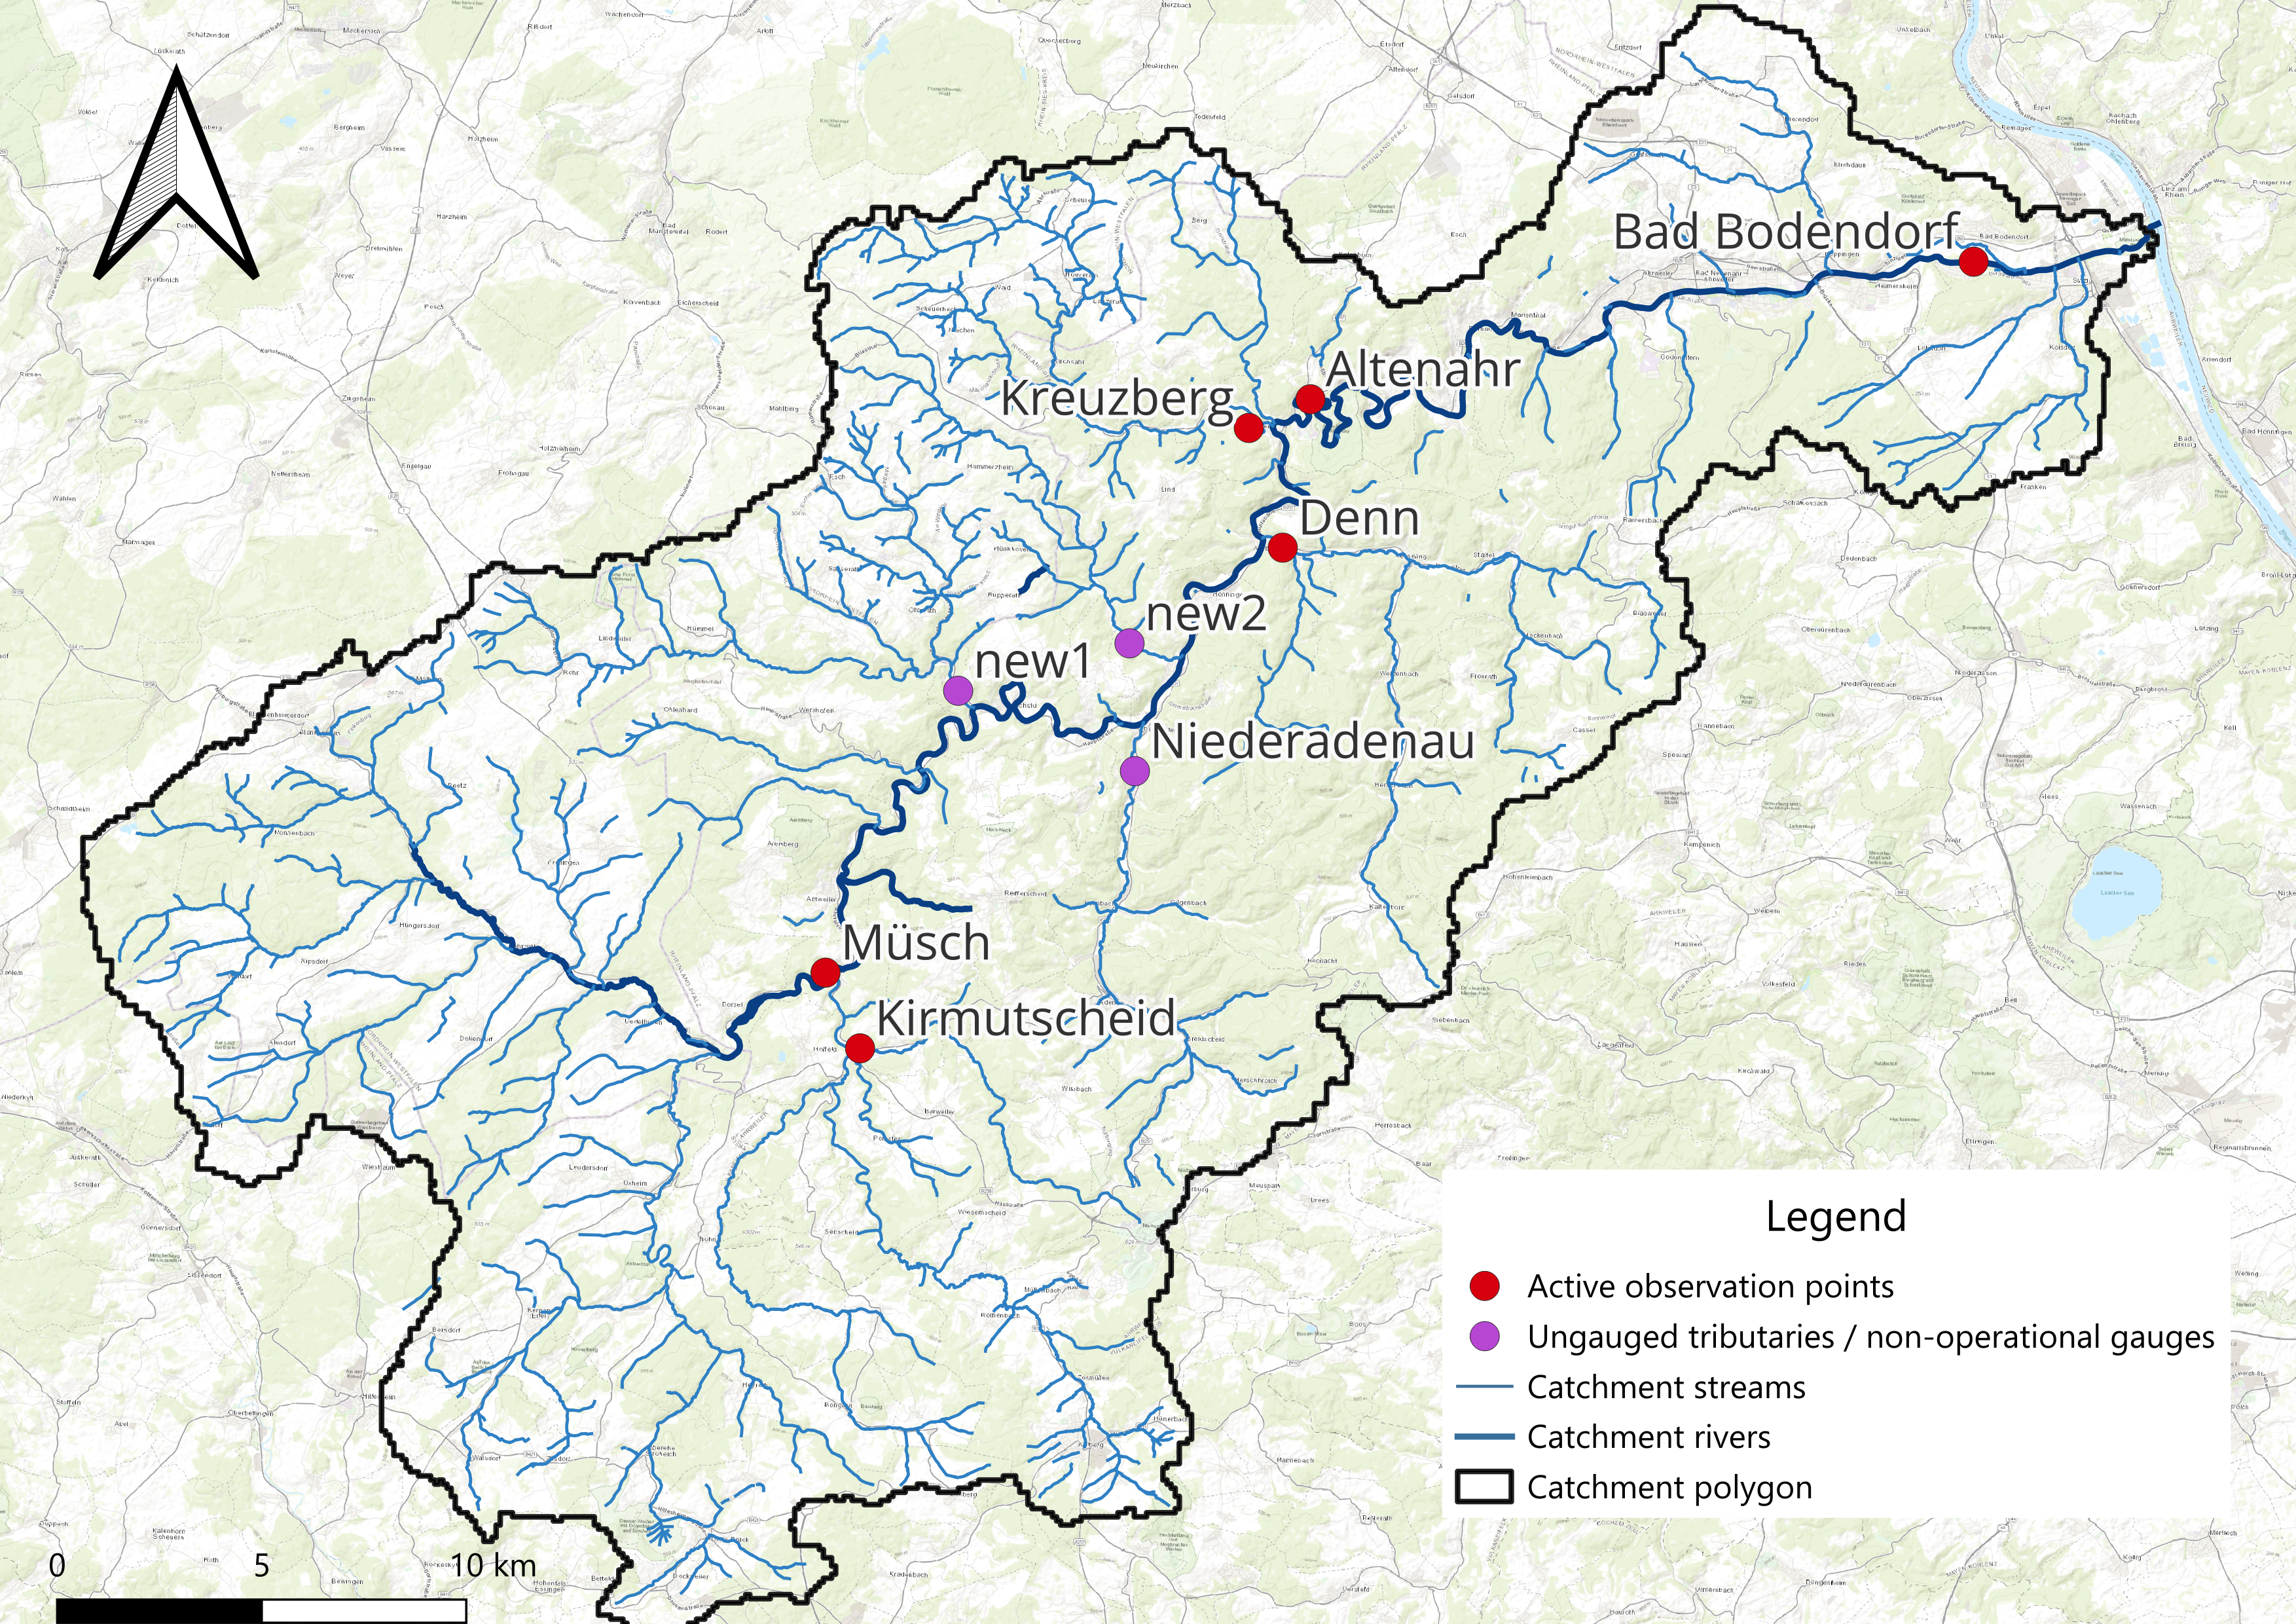
\includegraphics[width=0.7\textwidth]{observation stations.png}
    \caption{The Ahr catchment with the location of observation and inflow points used
    in this study: gauged/active (Altenahr, Kreuzberg, Denn, Kirmutscheid, M\"usch),
    gauged but data unavailable (Niederadenau), and ungauged (New1, New2).}
    \label{fig:observation_stations}
\end{figure}

\subsection{The July 2021 Flood Event}
\label{subsec:july2021}

The July 2021 flood was triggered by extratropical cyclone Bernd, which produced
100--150~mm of rainfall in the Ahr basin within 24 hours on 14--15 July, on top of
already saturated soils from weeks of above-average antecedent precipitation
\citep{kreienkamp2021rapid,mohr2023multidisciplinary}. The flood peak at Altenahr exceeded the statistical 100-year flood (HQ100) by a factor of about 4
\citep{mohr2023multidisciplinary}. The event killed 134 people in Rhineland-Palatinate and caused an
estimated 20 billion euros in damage to private property and public infrastructure \citep{lfurlp2022bericht}.

The gauge network was severely compromised during the event \citep{lfurlp2022bericht}. At
Altenahr, water levels rose from 13~cm/h in the early afternoon to 150~cm/h shortly
before the gauge failed at 20:45 on 14 July at a recorded level of 575~cm, several hours
before the actual peak around midnight. The M\"usch gauge failed earlier, with the main
sensor ceasing at approximately 15:30 and the redundant sensor recording a last value of
395~cm at 19:15 before transmission was lost. The Kreuzberg gauge was completely
destroyed. Of the four tributary gauges, only Denn and Kirmutscheid remained operational
throughout the event and provide reliable measured hydrographs. Peak levels and
discharges at the destroyed stations were reconstructed post-event from high-water mark
surveys, hydraulic back-calculations, and hydrological model simulations using LARSIM,
introducing considerable uncertainty particularly around the flood peak \citep{lfurlp2022bericht}.

For this study, the simulation period runs from 12 July 2021 00:00 to 17 July 2021
00:00 (five days), covering the full hydrograph. The combination of a narrow gorge,
multiple ungauged tributaries, saturated antecedent soils, and a destroyed gauging
station makes the Ahr 2021 event a demanding but instructive test case for a surrogate
model.

\section{SFINCS-Ahr Configuration}
\label{sec:sfincs_ahr_config}

This section applies the general methodology of Chapter~\ref{ch:methodology} to the
Ahr basin, giving the data sources, parameter values, and configuration decisions
used to set up SFINCS for the July 2021 flood event.

\subsection{Input Data}
\label{subsec:input_data_ahr}

The DEM used is a 1~m resolution LiDAR-derived terrain model reprojected to UTM zone
32N (EPSG:32632), used to define bed elevation at the computational grid level. The
model domain polygon is derived from HydroSHEDS catchment boundaries
\citep{lehner2008hydrosheds} and postprocessed in QGIS \citep{qgis2026}.
Because discharge hydrographs are used as boundary condition, the domain polygon is constructed
so that each inflow source point lies exactly on the catchment boundary. The seven inflow source points (four
gauged, three ungauged; Section~\ref{subsec:forcing_ahr}) were snapped to the nearest
point on the boundary polygon in QGIS. At the downstream end, a fixed water depth of
0~m is imposed at the outflow boundary to let water leave the domain freely.

\subsection{Forcing Data}
\label{subsec:forcing_ahr}

Rainfall from the RMI RADFLOOD21 product (1~km, 1~h resolution) was tested first as the
most physically complete representation of the flood-generating process \citep{beven2012rainfall},
before discharge hydrographs were adopted as the primary forcing type
(rationale: Section~\ref{subsec:forcing_data}). Observed 15-minute discharge records
were downloaded from the LfU RLP portal for the four gauged tributaries \citep{lfurlp2022bericht}.

\subsection{Ungauged Tributary Parameterisation}
\label{subsec:ungauged_ahr}

Comparing the sum of the four gauged tributary hydrographs against the observed
discharge at Altenahr revealed systematic underestimation, as expected: three
tributaries upstream of Altenahr with a combined area of $\approx$151~km$^2$ are absent
from the forcing. New1 and New2 have no gauge infrastructure, while Niederadenau is
gauged but its records could not be obtained for this study; all three are treated
identically for the purposes of discharge estimation and are referred to jointly as the
ungauged tributaries throughout this thesis. \textbf{Method 1} (Section~\ref{subsubsec:method1}) satisfies the selection
criteria (Section~\ref{subsec:ungauged}): it closes the mass balance at the outlet
exactly by construction, and requires no data beyond the gauged and outlet discharge
records already used for the other source points. It is therefore adopted as the
primary forcing for training and testing throughout this thesis, with $\Delta t =
1.5$~h derived from the cross-correlation lag between the gauged tributary sum and the
Altenahr record. \textbf{Methods 2 and 3} (Sections~\ref{subsubsec:method2}--\ref{subsubsec:method3})
are used exclusively for the sensitivity analysis of
Section~\ref{sec:physics_sensitivity_method}, to test the
model's response to alternative, more physically detailed forcing hypotheses at the
same locations. For Method~2, channel length $L$ and slope $S$ are measured from each
tributary confluence to Altenahr and converted into a routing lag $\Delta t_i$ via the
Kirpich formula (Eq.~\ref{eq:kirpich}); the resulting lags are given in
Table~\ref{tab:kirpich.
 
\begin{table}[H]
    \centering
    \caption{Kirpich routing lag parameters for ungauged source points.}
    \label{tab:kirpich}
    \begin{tabular}{lccc}
        \toprule
        \textbf{Point} & $L$ [km] & $S$ [m/m] & $\Delta t$ [h] \\
        \midrule
        New1         & 20.76 & 0.00427 & 5.6 \\
        Niederadenau & 14.23 & 0.00450 & 4.1 \\
        New2         & 12.42 & 0.00482 & 3.6 \\
        \bottomrule
    \end{tabular}
\end{table}
 
For Method 3, a curve number of $CN = 85$ (AMC-III) is applied, converted from $CN =
70$ (AMC-II, representative of mixed forest and agriculture on soil group B soils of
the Eifel region, \citealp{usdanrcs2004}, Ch.~7) using the standard AMC-III conversion
\citep{hawkins2009curvenumber}. AMC-III conditions (near-saturated antecedent soil moisture)
are justified by the two to three weeks of above-average precipitation preceding the
event \citep{kreienkamp2021rapid,mohr2023multidisciplinary}. Time to peak $T_p$ is estimated
with the Giandotti formula (Eq.~\ref{eq:giandotti}) from each subcatchment's area $A$,
longest flow path $L$, and relief $\Delta H$, and convolved with excess rainfall via
the triangular unit hydrograph (Eq.~\ref{eq:uh}) to give the parameters and resulting
peak discharges listed in Table~\ref{tab:uh_params}.
 
\begin{table}[H]
    \centering
    \caption{SCS unit hydrograph parameters for ungauged source points.}
    \label{tab:uh_params}
    \begin{tabular}{lcccccc}
        \toprule
        \textbf{Point} & $A$ [km$^2$] & $L$ [km] & $\Delta H$ [m] & $T_p$ [h] &
        $q_p$ [m$^3$/s/mm] & Peak $Q$ [m$^3$/s] \\
        \midrule
        New1         & 60.77 & 17.28 & 192.3 & 5.15 & 2.46 & 124 \\
        Niederadenau & 61.34 & 14.05 & 212.5 & 4.49 & 2.79 &  86 \\
        New2         & 29.45 & 13.76 & 171.6 & 4.04 & 1.17 &  72 \\
        \bottomrule
    \end{tabular}
\end{table}
 
\begin{figure}[H]
    \centering
    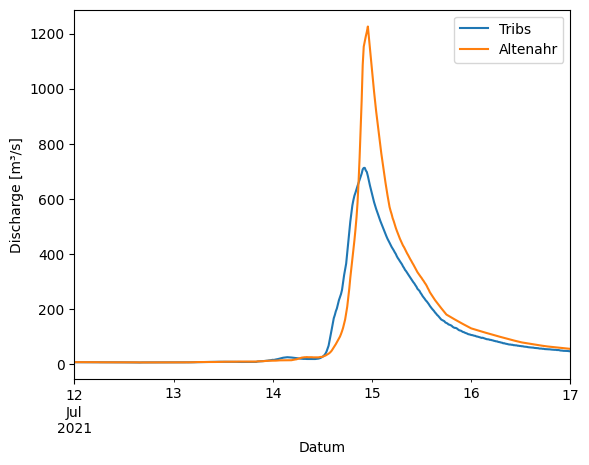
\includegraphics[width=0.7\textwidth]{tribs_vs_altenahr.png}
    \caption{Sum of the four gauged tributary discharges compared with the observed
    discharge at Altenahr during the July 2021 event, showing the systematic
    underestimation attributed to the three ungauged/unavailable tributaries
    (Section~\ref{subsec:ungauged_ahr}).}
    \label{fig:tribs_vs_altenahr}
\end{figure}

\begin{figure}[H]
    \centering
    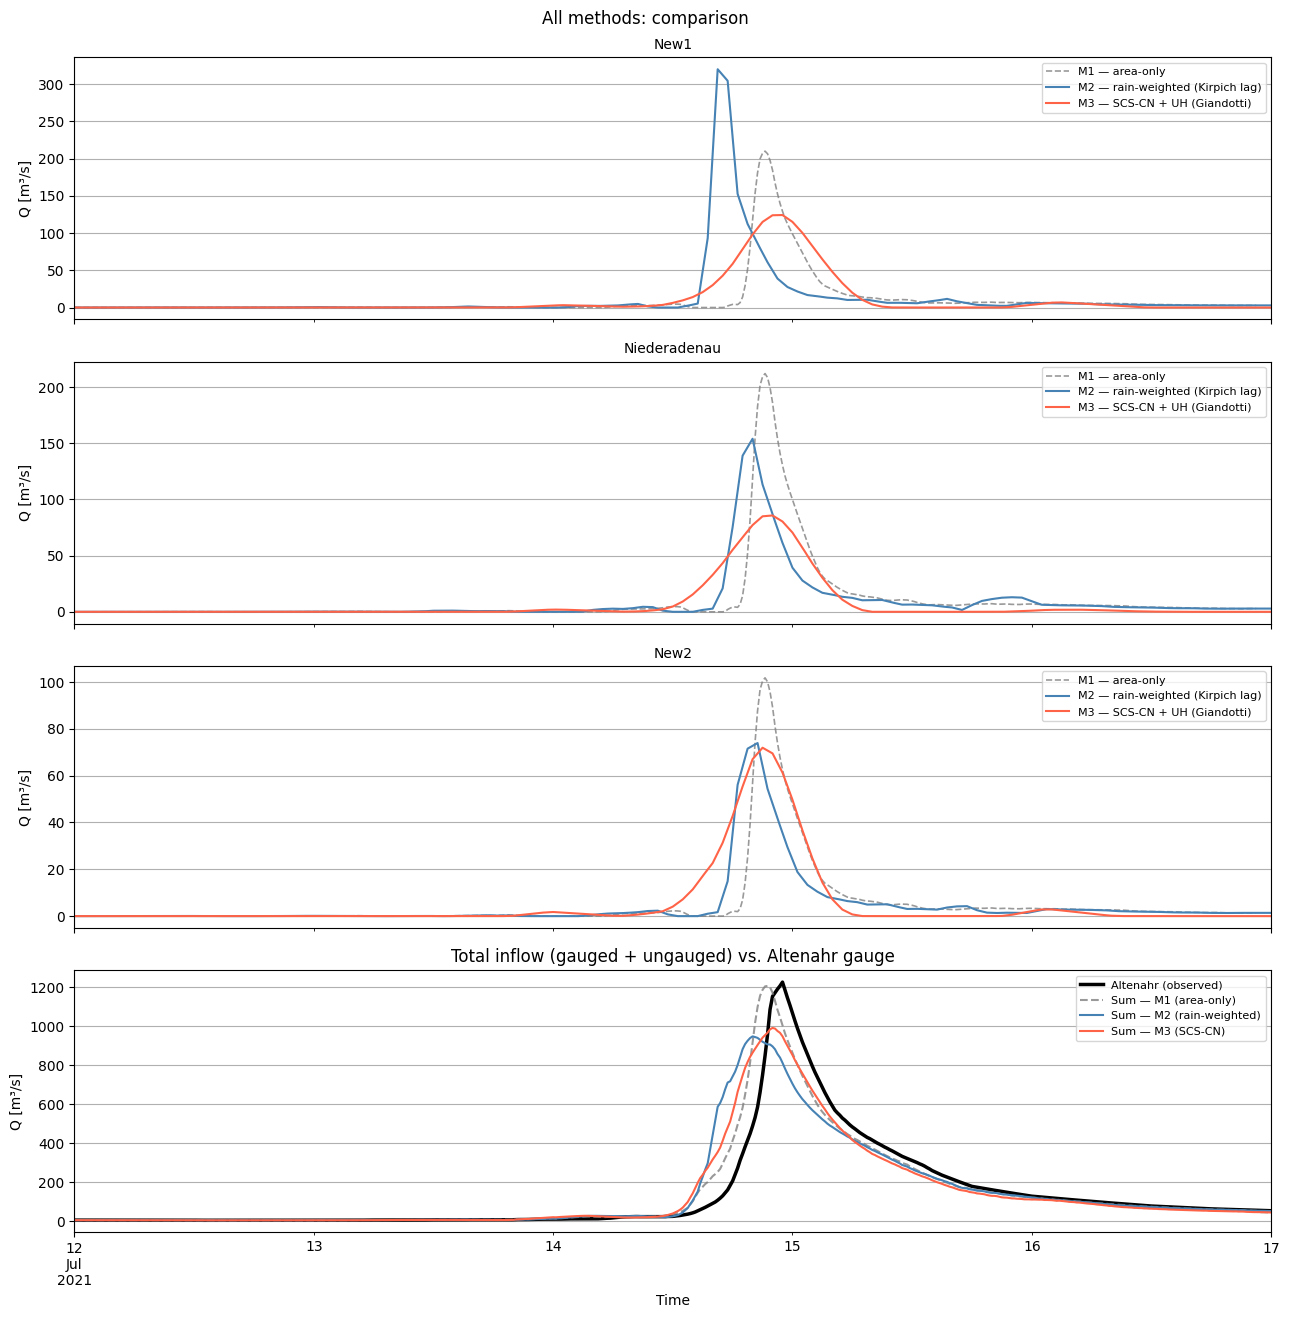
\includegraphics[width=0.8\textwidth]{comparison_methods_ungauged_tribs.png}
    \caption{Comparison of the discharge hydrographs estimated at the three ungauged
    source points (New1, Niederadenau, New2) by Methods~1--3.}
    \label{fig:comparison_methods_ungauged_tribs}
\end{figure}

\subsection{Grid, Subgrid, and Roughness}
\label{subsec:grid_ahr}

The SFINCS model is discretised at 100~m resolution over the Ahr basin domain
(Section~\ref{subsec:ahr_basin}). Subgrid lookup tables are derived from the 1~m LiDAR
DEM resampled to 2~m subgrid resolution. Roughness is assigned from the ESA WorldCover 2021 land-use map (10~m resolution;
\citealp{zanaga2022worldcover}), shown in Figure~\ref{fig:ahr_landuse}//, consistent
with the land-use characteristics described in Section~\ref{subsec:ahr_basin}.
Following \citet{arcement1989guide}, Manning's coefficients are assigned per class as:
forest and scrubland $n = 0.10$--$0.12$~m$^{-1/3}$s; agricultural and grassland
$n = 0.04$--$0.05$~m$^{-1/3}$s; built-up surfaces $n = 0.013$--$0.02$~m$^{-1/3}$s;
river channel $n = 0.035$~m$^{-1/3}$s.

Full numerical scheme parameter values used for the SFINCS-Ahr simulations are
listed in Appendix~\ref{app:sfincs_params}.
\textcolor{purple}{add pictures DEM and ESA land use}

\begin{figure}[H]
    \centering
    \includegraphics[width=0.7\textwidth]{ahr_dem.png}
    \caption{Digital elevation model of the Ahr basin domain, 1~m LiDAR-derived
    terrain reprojected to UTM zone 32N (EPSG:32632; Section~\ref{subsec:input_data_ahr}).}
    \label{fig:ahr_dem}
\end{figure}

\begin{figure}[H]
    \centering
    \includegraphics[width=0.7\textwidth]{ahr_landuse.png}
    \caption{ESA WorldCover 2021 land-use classification of the Ahr basin domain
    \citep{zanaga2022worldcover}, used to assign Manning's roughness coefficients.}
    \label{fig:ahr_landuse}
\end{figure}

\subsection{Initial Conditions and Warm-Start Procedure}
\label{subsec:warmstart_ahr}

A two-step warm-start procedure is adopted for the Ahr domain. First, a 144-hour
spinup simulation is run from 6 July 2021 00:00 to 12 July 2021 00:00, using the same
grid and subgrid setup as the flood simulation, with discharge held constant at the
pre-event baseflow values in Table~\ref{tab:spinup_baseflow}; ungauged source points
are assigned a small symbolic baseflow so that all inflow cells are hydraulically
active at $t=0$. The spinup is run to approximate steady state and the final model
state is saved as a restart file. Second, the flood simulation is initialised from
this restart, so that channels already carry baseflow at the start of the simulated
event.

\begin{table}[H]
    \centering
    \caption{Baseflow values used in the 144-hour spinup simulation.}
    \label{tab:spinup_baseflow}
    \begin{tabular}{llcc}
        \toprule
        \textbf{Source point} & \textbf{Type} & \textbf{Baseflow [m$^3$/s]} & \textbf{Source} \\
        \midrule
        Kreuzberg    & Gauged   & 0.461 & Observed ($t=0$, Section~\ref{subsec:forcing_ahr}) \\
        Denn         & Gauged   & 2.111 & Observed ($t=0$, Section~\ref{subsec:forcing_ahr}) \\
        Kirmutscheid & Gauged   & 2.780 & Observed ($t=0$, Section~\ref{subsec:forcing_ahr}) \\
        M\"{u}sch    & Gauged   & 0.645 & Observed ($t=0$, Section~\ref{subsec:forcing_ahr}) \\
        New1         & Ungauged & 0.100 & Symbolic (Section~\ref{subsec:ungauged_ahr}) \\
        Niederadenau & Ungauged & 0.100 & Symbolic (Section~\ref{subsec:ungauged_ahr}) \\
        New2         & Ungauged & 0.100 & Symbolic (Section~\ref{subsec:ungauged_ahr}) \\
        \bottomrule
    \end{tabular}
\end{table}

\subsection{SFINCS-Ahr Ground-Truth Validation}
\label{subsec:sfincs_validation_ahr}

The final SFINCS-Ahr configuration: seven tributary source points
(Sections~\ref{subsec:forcing_ahr}--\ref{subsec:ungauged_ahr}) initialised via the
spinup/warm-start procedure of Section~\ref{subsec:warmstart_ahr}, is validated
following the procedure of Section~\ref{subsec:sfincs_validation}. Gauge locations
are shown in Figure~\ref{fig:observation_stations}. The flood-extent product used is
a flood-affected-area shapefile covering the Ahr valley, dated 16 July 2021,
produced by the Center for Satellite Based Crisis Information (ZKI) of the German
Aerospace Center (DLR), derived from 10~cm-resolution post-event and 15~cm-resolution
pre-event aerial orthophotos, manually interpreted and validated by the ZKI mapping
team. A water-depth threshold of 0.1~m is used to classify simulated and reference
pixels as flooded; quantitative agreement (CSI) is reported in
Chapter~\ref{ch:results}.

\section{GNN Adaptation to the Ahr Mesh}
\label{sec:gnn_ahr}

The Ahr setup requires seven simultaneous inflow points (four gauged, three ungauged),
compared to the single breach ghost cell of the original dike-breach formulation
(method: Section~\ref{subsec:multiscale_mesh}). The SFINCS computational grid
(100~m resolution, active cells defined by $\mathrm{mask}>0$) is used directly as the
finest level of the multi-scale GNN mesh, retaining its structured square topology.
Three progressively coarser levels are constructed following the independent per-scale triangulation procedure of Section~\ref{subsec:model_adaptation_detail}, giving a
mesh hierarchy of approximately 100~m, 500~m, 1000~m, and 2000~m resolution ($K=4$
scales), designed to preserve the main topographic features of the catchment while
reducing computational complexity.

The dynamic-feature window is set to $p=3$ previous timesteps.
The training rollout length is increased
via curriculum learning to a final value of $r=5$ timesteps, chosen by balancing
training time against accuracy and stability, and consistent with the value used by
\citet{bentivoglio2025mswegnn}.
The learning rate follows a cosine-annealing schedule
($T_\text{max}=1000$, $\eta_\text{min}=1\times10^{-6}$) (Appendix~\ref{app:coslr}).


\paragraph{Cross-configuration generalisation test.} A model trained on one simulation configuration is evaluated, on simulations from a materially different configuration (e.g.\ including hydraulic structures). The model's response is expected to remain physically reasonable outside its training configuration.
 
\section{Computational Environment}
\label{sec:compute_environment}

All model training, hyperparameter sweeps, and the timing measurements underlying
the speed-up factor of Section~\ref{sec:benchmarking} were run on \texttt{hal8}, a
Deltares-managed high-performance computing cluster using the SLURM job scheduler.
Training and sweep jobs each requested one GPU (\texttt{gres=gpu:1}), 4 CPU
cores, 7500~MB of memory per core ($\approx$30~GB total), and a 24-hour
wall-clock limit, within the cluster's \texttt{gpu} partition.
GPU training and sweep jobs ran on an NVIDIA H100 NVL.  The CPU-side timing
measurements in Table~\ref{tab:speedup} used a separate, dedicated 4-vCPU
allocation (\texttt{4vcpu} partition) rather than the shared login node, chosen
to match the 4 threads SFINCS itself used for the same runs (confirmed from
each simulation's own \texttt{sfincs.log}, ``Using 4 of 4 available threads''),
so the CPU comparison in Table~\ref{tab:speedup} is between two solvers given
the same core budget. Jobs ran inside a dedicated conda
environment (Python 3.11, PyTorch~2.1.0, PyTorch Geometric~2.4.0, PyTorch
Lightning~2.1.0), managed via a \texttt{miniconda3} module. Experiment tracking
and the hyperparameter sweep of Appendix~\ref{app:hp_sweep} used Weights~\&~Biases.

All other work, dataset inspection, inference on already-trained checkpoints,
and figure generation, was carried out interactively on the author's own
machine, local work was restricted to CPU-only inference.


\section{Training Strategy Development}
\label{sec:training_strategy_dev}

This section documents, in chronological order, the sequence of experiments and
preliminary results that led from a naive application of mSWE-GNN to the final training configuration used for the
single-, four-, and twenty-simulation models evaluated in
Chapter~\ref{ch:results}.

\subsection{Zero-Shot and Fine-Tuning Baselines}
\label{subsec:zeroshot}

The pre-trained mSWE-GNN weights (DK15, \citealp{bentivoglio2025mswegnn}) were first
evaluated on the Ahr domain via direct forward inference, without any retraining, to
test whether the domain gap between the original dike-breach setting and the Ahr's
fluvial setting could be bridged without any adaptation at all. Fine-tuning from the
DK15 weights was tested next, as an intermediate step between direct transfer and
training entirely from scratch. Training from scratch was adopted as the reference
strategy for all subsequent experiments in this thesis (results and comparison:
Section~\ref{sec:zeroshot-finetune-coldwarm}).

\subsection{Initial-Condition Experiments}
\label{subsec:coldstart}

An initial from-scratch run tested a dry (cold-start) initial condition, following the original dike-breach formulation \citep{bentivoglio2025mswegnn}, to assess whether the surrogate could learn to initiate flow from an initially dry domain. The two-step spin-up/warm-start procedure (Section~\ref{subsec:warmstart_ahr}) was then adopted for all subsequent training. The effect of this choice is evaluated in Section~\ref{subsec:discussion_coldstart}.


\subsection{Loss and Hyperparameter Configuration}
\label{subsec:hyperparam_loss}

Starting from the warm-started dataset, the loss configuration was refined
following the comparisons described in Section~\ref{subsec:training_validation}. The final configuration used a shallow-water weight of $w=5$ to shallow wet cells with
water depths satisfying $0 < \text{WD} \le 0.30$~m. The mass-conservation penalty
was ultimately removed. The loss was retained across all four mesh scales rather
than restricted to the finest one, with per-scale weights $[5,1,1,1]$: the finest
scale, which determines the final predictions, is weighted five times more
heavily than the coarser scales, while the coarser scales still contribute to the
loss so that erroneous flood predictions there are penalised, since such errors
could otherwise propagate downward and degrade predictions at the finest scale.
The discharge output variable was weighted by $\gamma_\text{discharge}=7$ against
$\gamma_\text{depth}=1$ for water depth (Eq.~\ref{eq:forecast_loss}); this value was
held fixed at every stage of the loss configuration described above rather than
included in the sweep. This reference configuration was adopted for all subsequent
experiments.

The magnitude-scaling diagnostic of Section~\ref{sec:physics_sensitivity_method}
was then applied to this single-event model, to test whether its response tracked
forcing magnitude or simply reproduced the training event regardless of it
(results: Section~\ref{subsec:res_single_sim_sensitivity}). This test's outcome
motivated the multi-simulation training strategy described next.

\subsection{Multi-Simulation Training}
\label{subsec:multisimtraining}

Because a single-hydrograph model cannot be shown to use its forcing signal rather than
memorise the event (Section~\ref{subsec:hyperparam_loss}), a four-simulation training
set was generated by uniformly scaling the observed 2021 boundary hydrographs
(Sections~\ref{subsec:forcing_ahr}--\ref{subsec:ungauged_ahr}) by factors of 0.5, 0.75,
1.25, and 1.5, keeping the SFINCS domain, mesh, nearest-neighbour ghost-cell mapping,
and warm-start procedure otherwise unchanged. The model was trained on the four scaled
simulations and validated/tested on the unscaled ($1\times$) event, so reported test
metrics reflect performance on a hydrograph magnitude not seen during training.

Applying the diagnostics of Section~\ref{sec:physics_sensitivity_method} to the four-simulation model motivated a third training dataset (results: Section~\ref{sec:res_four_sim_magnitude_sensitivity}--\ref{subsec:res_four_sim_sensitivity}).

The third dataset was constructed as a set of discrete, hand-designed perturbations:

\begin{itemize}
    \item The four existing uniformly-scaled events (0.5$\times$, 0.75$\times$, 1.25$\times$, 1.5$\times$, applied to all seven boundary sources together) retained unchanged, so that the whole-catchment magnitude scaling already learned is not lost.
    \item Eleven per-tributary magnitude perturbations: each of the seven boundary-condition source locations scaled individually, holding the other six at 1$\times$. For the four locations the sensitivity ladder flagged as most clearly under-responsive (Kirmutscheid, Kreuzberg, Niederadenau, and the smallest tributary ``new2''), the ladder was extended down to 0$\times$ (source switched off) as well.
    One combined-perturbation event, included so that the training set contains at least one genuinely multi-source combination
    This directly targets the per-source diagnostic limitation, by forcing the network to attribute response magnitude to the specific node an inflow enters at, rather than to an aggregate forcing signal.
    
    \item A timing-perturbation pair, shifting the rise time of the dominant tributary (Kirmutscheid) by $\pm$50\% (8~h to 12~h, and the reciprocal contraction), together with one all-locations-desynchronised event in which every source's timing offset is varied independently, so that forcing variation is not limited to magnitude alone.
    
    \item One catchment-emptying event (``all-drain''), initialised from the pre-event baseline and rolled out for an extended horizon ($\sim$450 steps, versus $\sim$120 for the other events) until the domain fully drains, directly addressing the recession-test limitation.
\end{itemize}

Two further scenarios were generated but deliberately withheld from training as a held-out compositional-generalisation test set: an all-locations desynchronisation with every timing offset reversed relative to the training event, and a second draining scenario initialised from the flood peak rather than the pre-event baseline.

\subsection{Run-to-Run Variability}
\label{subsec:seed_ruler_ahr}

Differences between two configurations can be of a similar order to what plausibly
arises from stochastic training alone (weight initialisation, batch ordering), rather
than reflecting the design choice being compared. To provide an empirical reference
for this run-to-run variability, a chosen reference configuration is retrained several
times with all hyperparameters held fixed, varying only the random seed. Configuration comparisons whose reported difference
falls within this spread cannot be attributed to the design choice being tested with
confidence, whereas differences clearly outside it are more likely to reflect a
genuine effect.

A single fixed baseline configuration, reached after fixing shallow-weighted RMSE
($w=5$) and removing the mass-conservation penalty, with loss computed on the finest
scale only, was retrained five times with all hyperparameters held fixed, varying
only the random seed (1, 200, 450, 666, 800). Given that only five seeds were
evaluated, the resulting spread should be treated as an approximate empirical bound
rather than a robust variance estimate; the spread is used in
Chapter~\ref{ch:results} to qualify which configuration comparisons reflect a
genuine effect.

\begin{table}[H]
  \centering
  \caption{Seed-to-seed variability reference band: mean $\pm$ standard
    deviation, with range in brackets, across 5 seeds of the reference configuration.}
  \label{tab:seed reference band}
  \begin{tabular}{lc}
    \toprule
    Metric & Best val.\ loss ($n=5$)  \\
    \midrule
    RMSE WD [m] & $0.142 \pm 0.010$ \; [0.127, 0.154] \\
    CSI@0.05    & $0.703 \pm 0.029$ \; [0.666, 0.730] \\
    CSI@0.30    & $0.832 \pm 0.016$ \; [0.811, 0.857] \\
    \bottomrule
  \end{tabular}
  \\[4pt]
  \footnotesize Best epochs:  $=$ 922, 546, 541, 668, 660; .
\end{table}



\section{Hydraulic Structure Scenario Design}
\label{sec:structure_scenarios}

Once the model reached adequate baseline performance on the twenty-simulation dataset,
it was retrained on an augmented dataset including hydraulic structures, following the
representation methods of Section~\ref{sec:hydraulic_structures_method}, with no
changes to training hyperparameters, loss configuration, or curriculum schedule beyond
the training dataset itself.

Following the functional roles defined in Section~\ref{subsec:whatif_framework},
structures were placed at two locations chosen for hydraulic and social relevance to
the 2021 event: two levees along the river margin through Bad Neuenahr-Ahrweiler, in a
district where an estimated 75\% of the affected area was flooded during the event
\citep{schafer2021cedim}, and two flow obstructions (weirs) in the Altenahr area, where several bridges failed
under hydraulic loading and debris accumulation during the event, blocking flow \citep{mohr2023multidisciplinary}.

\textcolor{blue}{note: add map figure showing structure locations or keep in the appendix?, picture of failed bridges?}

Sixteen structure scenarios were generated in total: twelve used for training and four
held out for testing (Table~\ref{tab:structure_scenarios}). Across
both locations, scenarios varied structure length, position, and crest elevation; crest
heights, measured above the channel bed, were deliberately swept up to intentionally
extreme values of 15~m and 20~m (for the flow obstruction scenarios), exposing the model to a wide range of structure
heights. The four held-out test simulations reuse the
same structure types seen during training but place them in a new, unseen location,
assign a new, unseen crest elevation, or introduce a breach in the structure itself, so
that performance can be assessed on structure configurations not encountered during
training. The retrained structure-aware model uses a training dataset of 32 SFINCS
simulations in total.

%\section{Experimental Design Summary}
%\label{sec:experiment_design_table}

%Table~\ref{tab:experiment_design} maps every experiment introduced in this chapter to
%the section of Chapter~\ref{ch:results} where its results are reported and the
%sub-question (Section~1.4) it primarily addresses.

%\begin{table}[h]
%    \centering
%    \caption{Experimental design summary: experiment, configuration, and target Results section / sub-question.}
%    \label{tab:experiment_design}
%    \begin{tabular}{lllc}
%        \toprule
%        \textbf{Experiment} & \textbf{Section (this ch.)} & \textbf{Results \S} & \textbf{SQ} \\
%        \midrule
%        SFINCS-Ahr ground-truth validation & \ref{subsec:sfincs_validation_ahr} & \S5.1 & SQ4 \\
%        Zero-shot / fine-tune baseline      & \ref{subsec:zeroshot}             & \S5.2 & SQ1, SQ4 \\
%        Cold-start vs.\ warm-start          & \ref{subsec:coldstart}            & \S5.2 & SQ1 \\
%        Seed variability (run-to-run ruler) & \ref{subsec:seed_ruler_ahr}       & \S5.3 & SQ3, SQ4 \\
%        Loss/hyperparameter ablation        & \ref{subsec:hyperparam_loss}      & \S5.4 & SQ1, SQ3 \\
%        Single-simulation model             & \ref{subsec:hyperparam_loss}      & \S5.5 & SQ3, SQ4 \\
%        Physics sensitivity (single-sim)    & \ref{sec:physics_sensitivity_method} & \S5.5 & SQ4 \\
%        Four-simulation model               & \ref{subsec:multisimtraining}     & \S5.6 & SQ4 \\
%        Physics sensitivity (four-sim)      & \ref{sec:physics_sensitivity_method} & \S5.6 & SQ4 \\
%        Twenty-simulation model             & \ref{subsec:multisimtraining}     & \S5.7 & SQ3, SQ4 \\
%        Hydraulic structures                & \ref{sec:structure_scenarios}     & \S5.8 & SQ2, SQ5 \\
%        Ensemble / probabilistic runs (if time allows) & --                     & \S5.9 & SQ6 \\
%        \bottomrule
%    \end{tabular}
%\end{table}
%\bigskip
\noindent The following chapter reports and discusses the results of each of these
experiments in turn, following the same chronological order.

\section{Summary Table of training configurations}

\begin{table}[H]
    \centering
    \caption{Overview of training configurations used throughout this thesis.
    M = BC magnitude variability, S = BC per-source variability, T = BC timing
    variability, R = recession/drainage scenario, D = hydraulic structures.}
    \label{tab:training_configs_overview}
    \begin{tabular}{lccccccl}
        \toprule
        \textbf{Configuration} & \textbf{\# Sims} & \textbf{M} & \textbf{S} & \textbf{T} & \textbf{R} & \textbf{D} & \textbf{Evaluated on} \\
        \midrule
        Single-simulation & 1  & No  & No  & No  & No  & No  & Training event (1$\times$) \\
        Four-simulation   & 4  & Yes & No  & No  & No  & No  & Held-out 1$\times$ event \\
        Twenty-simulation & 20 & Yes & Yes & Yes & Yes & No  & Held-out 1$\times$ event \\
        Structure-aware   & 32 & Yes & Yes & Yes & Yes & Yes & \shortstack{Held-out 1$\times$ event\\+ structure scenarios} \\
        \bottomrule
    \end{tabular}
\end{table}

%================================================================
% CHAPTER 5: RESULTS
%================================================================
 
\chapter{Results and Discussion}
\label{ch:results}
 
Each section reports results and discusses them immediately.
 
Unless noted otherwise, all metrics in this chapter are computed on the test split
defined in Section~\ref{subsec:temporal_resolution}. For the single-simulation
configurations of Sections~\ref{sec:zeroshot-finetune-coldwarm}--\ref{sec:res_hyperparam},
training, validation, and test all draw on the same 2021 event. From
Section~\ref{sec:res_four_sim} onward, the model is trained on multiple scaled and
perturbed simulations and evaluated on the unscaled warm-started 2021
event, held out entirely from training; metrics reported there do reflect performance
on forcing not seen during training.
 
 
\section{SFINCS-Ahr Ground-Truth Validation}
\label{sec:res_sfincs_validation}
 
Table~\ref{tab:gauge_validation} compares the simulated and observed water-depth
records at the two gauge stations with a continuous observed depth record spanning the
event window (12--17 July 2021): Altenahr, upstream and closest to the gauged tributary
inflows, and Bad Bodendorf, at the catchment outlet. RMSE (Eq.~\ref{eq:rmse}) is
computed over the full window on paired timestamps, with the observed record linearly
interpolated onto the simulation's hourly output times.
 
\begin{table}[H]
    \centering
    \caption{Simulated vs.\ observed peak water depth, timing offset and RMSE at
    the two gauge stations with continuous observed depth records, warm-started
    SFINCS-Ahr simulation, 12--17 July 2021.}
    \label{tab:gauge_validation}
    \begin{tabular}{lccccc}
        \toprule
        \textbf{Station} & \textbf{Peak sim.} & \textbf{Peak obs.} & \textbf{Peak error} & \textbf{Timing offset} & \textbf{RMSE} \\
         & [m] & [m] & [m (\%)] & [h] & [m] \\
        \midrule
        Altenahr       & 8.48 & 9.84 & $-1.36$ ($-13.8\%$) & $+1.3$ & 1.31 \\
        Bad Bodendorf  & 3.48 & 4.85 & $-1.37$ ($-28.3\%$) & $+2.3$ & 0.73 \\
        \bottomrule
    \end{tabular}
\end{table}
 
\noindent
At both stations, the simulated peak water depth underestimates the observed peak, and
the simulated peak arrives later than observed, with a larger
relative error and lag at Bad Bodendorf ($-28.3\%$, $+2.3$~h) than at Altenahr
($-13.8\%$, $+1.3$~h). However, the full-window RMSE alone masks how this
error is distributed in time at the two stations: Figure~\ref{fig:gauge_timeseries}
plots the full simulated and observed series over the event window, and
Table~\ref{tab:gauge_bias_decomp} decomposes the mean residual (simulated minus
observed) into a window within $\pm 12$~h of the observed peak and the remainder of the
record.
 
\begin{figure}[H]
    \centering
    \begin{subfigure}{0.85\textwidth}
        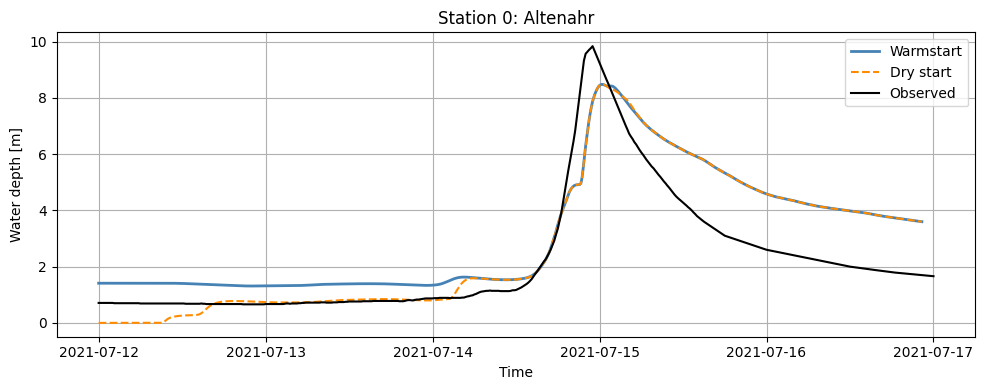
\includegraphics[width=\linewidth]{5.1_altenahr_simVSobs.png}
        \caption{Altenahr}
    \end{subfigure}
    \\[0.5em]
    \begin{subfigure}{0.85\textwidth}
        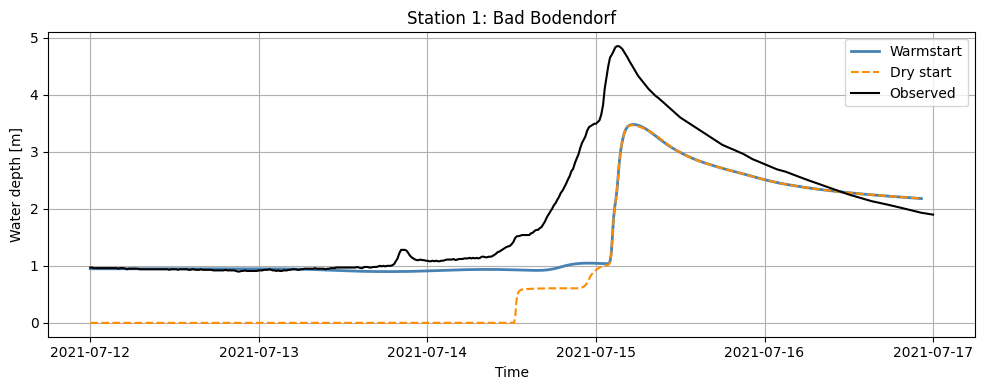
\includegraphics[width=\linewidth]{5.1_BadBodendorf_simVSobs.png}
        \caption{Bad Bodendorf}
    \end{subfigure}
    \caption{Simulated (warm-started and dry-start) vs.\ observed water depth,
    12--17 July 2021.}
    \label{fig:gauge_timeseries}
\end{figure}
 
\begin{table}[H]
    \centering
    \caption{Decomposition of the mean residual (simulated $-$ observed, in m) into a
    window within $\pm 12$~h of the observed peak and the remainder of the record.}
    \label{tab:gauge_bias_decomp}
    \begin{tabular}{lccc}
        \toprule
        \textbf{Station} & \textbf{Near peak ($\pm 12$~h)} & \textbf{Elsewhere} & \textbf{Full window} \\
        \midrule
        Altenahr       & $+0.05$ & $+1.14$ & $+0.92$ \\
        Bad Bodendorf  & $-1.34$ & $-0.10$ & $-0.35$ \\
        \bottomrule
    \end{tabular}
\end{table}
 
\noindent
%The two stations show essentially opposite error structures.
At Altenahr, the recession
limb drains markedly more slowly than observed, so the mean residual away from the peak is strongly
positive ($+1.14$~m). Only in a narrow window at the observed peak itself does the
simulation fall behind, at the moment of the observed peak (14 July 23:00) simulated
depth is 7.87~m against an observed 9.84~m.
 
At Bad Bodendorf the response to the
flood itself is both delayed and strongly damped (at 15 July 00:00, while the
observed record is already rising through 3.49~m, the simulation is still at 1.04~m)
concentrating almost all of the station's error into the peak window ($-1.34$~m mean
residual, RMSE 1.57~m within $\pm 12$~h vs.\ 0.21~m outside it). The same slow-emptying
behaviour seen at Altenahr is present at Bad Bodendorf too, the
observed recession outpaces the simulated one by a factor of roughly 2--3 through the
second half of the window.
 
\subsection{Flood Extent Agreement with the ZKI Product}
\label{subsec:results_csi}
 
Figure~\ref{fig:simulated_observed_flood_reach} shows the SFINCS-simulated maximum water extent (depth threshold 0.1~m) alongside the ZKI flood-affected-area shapefile (Section~\ref{subsec:sfincs_validation_ahr}).
Table~\ref{tab:csi_validation} reports
the resulting pixel counts and CSI (Eq.~\ref{eq:csi}), both over the full model domain
and after excluding the downstream-most reach where the false positives are
concentrated.
 
\begin{table}[H]
    \centering
    \caption{Flood extent agreement (pixel counts and CSI) between the SFINCS-Ahr
    maximum water extent and the ZKI flood-affected-area product.}
    \label{tab:csi_validation}
    \begin{tabular}{lcccc}
        \toprule
        \textbf{Extent} & \textbf{TP} & \textbf{FP} & \textbf{FN} & \textbf{CSI} \\
        \midrule
        Full domain              & 101{,}581 & 82{,}568 & 8{,}252 & 0.528 \\
        Excl.\ downstream reach  & 101{,}581 & 30{,}104 & 8{,}252 & 0.726 \\
        \bottomrule
    \end{tabular}
\end{table}
 
 
\begin{figure}[H]
    \centering
    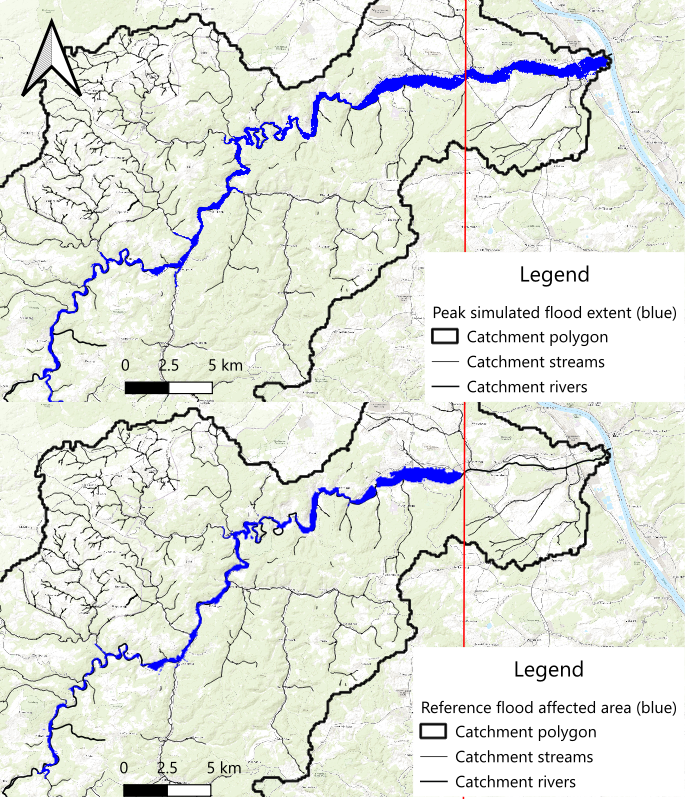
\includegraphics[width=0.8\textwidth]{simulated_observed_flood_reach.png}
    \caption{Simulated (SFINCS-Ahr) versus ZKI-observed flood extent along the Ahr
    valley. The red line marks the downstream-most extent of the ZKI reference
    product, beyond which the observed flood extent is missing from the ZKI mapping.}
    \label{fig:simulated_observed_flood_reach}
\end{figure}
 
Over the full domain, CSI is 0.528, with false positives (82{,}568 pixels) far
outnumbering false negatives (8{,}252 pixels). TP and FN are unchanged when the
downstream-most reach of the model domain (a straight-line distance of
$\approx$8.1~km, corresponding to a simulated flood extent of 5.25~km$^2$) is
excluded, while FP falls by 63\% (from 82{,}568 to 30{,}104), raising CSI to 0.726.
This location is not arbitrary: the ZKI reference
product's own mapped flooded area ends where
the reach exclusion begins. Within the reduced area on which the ZKI product and the simulation can
actually be compared, the simulated and ZKI-mapped flood extents agree closely
(CSI~$=0.726$).
 
\subsection{Discussion: Phase-Dependent, Station-Specific Bias in Gauge Water Depth}
\label{subsec:discussion_gauge}
 
The peak-only comparison in Table~\ref{tab:gauge_validation} understates how different
the two stations' error behaviour actually is once the full time series
(Figure~\ref{fig:gauge_timeseries}) and the near-peak/elsewhere bias decomposition
(Table~\ref{tab:gauge_bias_decomp}) are examined: the simulation is biased in
opposite directions, at the two stations.
 
At \textbf{Bad Bodendorf}, three separate mechanisms plausibly contribute, two of which
act on the peak and one on the recession.
 
One candidate for the peak is that a 100~m grid cell is simply too wide relative to the
real river channel. At $t=0$ baseflow, the model's cross-sectional discharge is
2--6$\times$ higher than the observed baseflow for the same water level,  the real
channel evidently occupies only a fraction of one grid cell's width, so the model
over-estimates how much a given water level can convey. This mismatch does not carry
over cleanly to high flow: at high flow the real
river has overtopped its banks and genuinely occupies a width closer to the model's
100~m cell, narrowing the low-flow gap, it means the low-flow diagnostic
does not, on its own, explain why the simulated peak \emph{stage} falls short
 
A more direct candidate for the peak is the model's outflow boundary condition. The domain's downstream boundary is set to a fixed
water depth of 0~m to allow free outflow (Section~\ref{subsec:input_data_ahr}). Bad Bodendorf sits only $\approx$4.5~km from the
outflow boundary, well
within range for the fixed-zero-depth condition to distort the backwater curve
there, which would suppress and delay the simulated peak. 
%Both mechanisms point the same direction and are not
%mutually exclusive; distinguishing their relative contribution is not possible from
%gauge data alone and would require inspecting the simulated water-surface profile
%approaching the outflow boundary directly.
 
The mechanism for the recession is different again: a slower-than-observed emptying
rate. This is the same mechanism that dominates at
Altenahr, discussed next.
 
At \textbf{Altenahr}, an unconfirmed mechanisms is plausible here: the markedly slower
recession (4.59~m simulated vs.\ 2.60~m observed at 16 July 00:00, and the same
relative-rate lag identified at Bad Bodendorf above) points to the model retaining
floodwater longer than the real river, for which channel roughness
(Section~\ref{subsec:roughness}), and floodplain storage at the 100~m grid
resolution are all candidate contributors.
 
The two stations therefore share the slow-emptying recession bias, but differ in which
mechanism dominates their full-window residual.
 
\subsection{Discussion: The Downstream Flood-Extent Discrepancy, An Open Question}
\label{subsec:discussion_csi}
The flood-extent comparison (Section~\ref{subsec:results_csi}) shows the opposite sign
of disagreement in the downstream-most reach from the one where the gauge comparison
shows underestimation: nearly all of the apparent false-positive area (52{,}464 of
82{,}568 pixels, 5.25~km$^2$) is concentrated there, i.e.\ the model appears to
\emph{over}-predict flood extent in roughly the reach where it \emph{under}-predicts
flood depth at the nearby Bad Bodendorf gauge.
 
That tension is largely resolved by checking where the reference data itself actually
extends: the ZKI product's own mapped flooded pixels stops where the
reach exclusion that recovers CSI~$=0.726$ begins.
Under a raster classification that treats "no ZKI polygon" as
"not flooded" (Section~\ref{subsec:results_csi}), every simulated wet pixel beyond that
line is scored as a false positive by construction. 
The stretch could additionally have been largely unaffected in reality,
independent of reference coverage; and the downstream boundary condition could still contribute a larger simulated flooded area on
top of the coverage artifact
(Section~\ref{subsec:discussion_gauge}). 
 
The full-domain CSI ($0.528$) should be treated as an artifact of comparing against absent
reference data rather than a measure of model skill, and the reduced-area CSI
($0.726$) is the only figure that reflects an actual comparison. GNN training data
drawn from this downstream-most reach should still be treated with more caution than
data from the rest of the domain.


 
% -> Answers: SQ4 (foundation for "how well does it perform on the Ahr catchment" --
%    establishes ground-truth quality before the surrogate is judged against it)
 
\section{Zero-Shot, Fine-Tuning, and Cold-/Warm-Start}
\label{sec:zeroshot-finetune-coldwarm}
 
Table~\ref{tab:baseline-strategies} reports outcomes for every baseline strategy tested
before adopting warm-started training from scratch as the reference configuration
(rationale and mechanism: Sections~\ref{subsec:zeroshot}--\ref{subsec:coldstart}; full
rollout figures in Appendix~A).  Zero-shot DK15 inference collapsed to CSI~$=0.000$ at every threshold.
Fine-tuning from DK15, under matched architecture, trailed training from scratch at
both checkpoints. Cold-start training from scratch collapsed to a near-all-dry
prediction. Only once training used the warm-started ground truth did CSI on the
training event reach a usable range, motivating its adoption as standard for all
subsequent training (Section~\ref{subsec:hyperparam_loss}).
 
\begin{table}[H]
  \centering
  \caption{Baseline strategy comparison: zero-shot transfer, fine-tuning vs.\ training
    from scratch, and cold- vs.\ warm-start initialisation.}
  \label{tab:baseline-strategies}
  \begin{tabular}{lccc}
    \toprule
    Configuration & RMSE WD [m] & CSI@0.05 & CSI@0.30 \\
    \midrule
    Zero-shot (DK15, no retraining)                     & 0.147            & 0.000         & 0.000 \\
    Fine-tuned from DK15              & 0.191  & 0.666  & 0.778  \\
    From scratch, matched arch.\       & 0.096  & 0.828  & 0.898  \\
    Cold-start, from scratch           & 0.195  & 0.054  & 0.024  \\
    Warm-start, from scratch (reference config)          & 0.4703            & 0.589         & 0.561 \\
    \bottomrule
  \end{tabular}
\end{table}
 
 
\textcolor{red}{maybe delete this full sub section... and just include them in annex A with pictures od the this runs simulations}
 
\subsection{Discussion: Cold-Start Failure}
\label{subsec:discussion_coldstart}

The cold-start run converged to a degenerate solution: the model produced no
inundation throughout the autoregressive rollout, regardless of training duration or
hyperparameter setup (Table~\ref{tab:baseline-strategies}). With upstream
point-source forcing and a fully dry domain at $t=0$, there is no spatial hydraulic
gradient for the model to propagate, and the large proportion of permanently dry
cells yields an artificially low loss for the trivial all-dry prediction. This is
consistent with the message-passing update of
Equations~\ref{eq:message}--\ref{eq:node_update}: the gradient term suppresses flux
from cells that carry no water, so a fully dry state offers the network nothing to
propagate from a point-source ghost cell. Read this way, the result points to a
genuine limitation of the architecture itself: it propagates and amplifies existing
water effectively, but doesn't reliably initiate flow from a dry state.

This architectural explanation is not the only one available. The cold-start test was run using only the single
available training simulation, before the four- and twenty-simulation datasets
(Section~\ref{subsec:multisimtraining}) were introduced, and every model in this
thesis trained on a single simulation showed some form of degenerate or narrowly
memorised behaviour (Section~\ref{subsec:res_single_sim_sensitivity}), independent of
initial condition. It is therefore possible that the cold-start failure was, at least
in part, a symptom of limited training diversity rather than purely of the dry-state
message-passing limitation described above: with only one event's worth of dry-to-wet
transitions available, the model may simply never have seen enough varied examples
of flow initiation to learn it, regardless of architecture.

With warm-started ground truth, training became stable and CSI on the training event
rose into a usable range.
% DK15 zero-shot CSI=0 result; fine-tune vs scratch comparison (Appendix B.1);
% cold-start degenerate-solution result; warm-start fix.
% -> Answers: SQ1 (what adaptations are required to extend mSWE-GNN to fluvial flooding)
 
\section{Loss and Hyperparameter Configuration}
\label{sec:res_hyperparam}
 
Every comparison in this section is judged against the seed-to-seed reference band
established in Section~\ref{subsec:seed_ruler_ahr} (Table~\ref{tab:seed-ruler}): a
difference smaller than the band's width cannot be attributed to the design choice being tested with confidence.
 
\paragraph{Shallow-water-weighted vs.\ unweighted RMSE.}
Removing the shallow-cell weighting ($w=1$ instead of $w=5$ for $0 < \mathrm{WD} \le
0.30$~m) falls below the reference band range (Table~\ref{tab:seed-ruler}). Weighting shallow wet cells was
retained.
 
\begin{table}[H]
  \centering
  \caption{Unweighted RMSE ($w=1$) vs.\ the reference band range (Table~\ref{tab:seed-ruler}),
    best val.\ loss checkpoint.}
  \label{tab:unweighted-rmse}
  \begin{tabular}{cccc}
    \toprule
    RMSE WD [m] & CSI@0.05 & CSI@0.30 & vs.\ reference band \\
    \midrule
    0.155 & 0.660 & 0.804 & below \\
    \bottomrule
  \end{tabular}
\end{table}
 
\paragraph{Mass-conservation penalty.}
Re-introducing the mass-conservation penalty ($\lambda = 0.01$, Eq.~\ref{eq:mass_loss})
falls below the reference band range. It was removed from the reference
configuration.
 
\begin{table}[H]
  \centering
  \caption{Mass-conservation penalty on ($\lambda=0.01$) vs.\ the reference band range
    (Table~\ref{tab:seed-ruler}), best val.\ loss checkpoint.}
  \label{tab:conservation}
  \begin{tabular}{cccc}
    \toprule
    RMSE WD [m] & CSI@0.05 & CSI@0.30 & vs.\ reference band \\
    \midrule
    0.184 & 0.614 & 0.763 & below \\
    \bottomrule
  \end{tabular}
\end{table}
 
 
\paragraph{Loss on all mesh scales vs.\ the finest scale only.}
Supervising all four mesh scales (weights $[5,1,1,1]$, finest first) rather than only
the finest lands above the reference band range (Table~\ref{tab:multiscale-loss}). Since coarse-scale
errors can propagate downward through the processor's upsampling branch
(Section~\ref{subsec:processor}) and degrade the finest-scale prediction, negatively impacting the test metrics.
 
\begin{table}[H]
  \centering
  \caption{All-scale weighted loss ($[5,1,1,1]$, seed 200) vs.\ the reference band range
    (Table~\ref{tab:seed-ruler}), best val.\ loss checkpoint.}
  \label{tab:multiscale-loss}
  \begin{tabular}{cccc}
    \toprule
    RMSE WD [m] & CSI@0.05 & CSI@0.30 & vs.\ reference band \\
    \midrule
    0.158 & 0.775 & 0.832 & above \\
    \bottomrule
  \end{tabular}
\end{table}
 
\begin{table}[H]
  \centering
  \caption{RMSE WD per mesh scale (s0~=~finest, s3~=~coarsest), finest-scale-only loss
    vs.\ all-scale loss, both at the best-val.-loss checkpoint. Coarse scales are
    effectively unsupervised under finest-only loss.}
  \label{tab:multiscale-perscale}
  \begin{tabular}{lcccc}
    \toprule
    Loss configuration & RMSE s0 & RMSE s1 & RMSE s2 & RMSE s3 \\
    \midrule
    Finest-only   & 0.198 & 0.368 & 0.482 & 0.620 \\
    All-scale     & 0.203 & 0.200 & 0.161 & 0.213 \\
    \bottomrule
  \end{tabular}
\end{table}
\textcolor{blue}{note:maybe delete this table (5.8)...?}
 
\paragraph{Four vs.\ three mesh scales.}
Removing the coarsest ($\sim$2000~m) level degraded performance
relative to the four-scale reference (Table~\ref{tab:threescale}), introducing a delay in the simulated flood front. Four scales were retained.
 
\begin{table}[H]
  \centering
  \caption{Four vs.\ three mesh scales (coarsest $\sim$2000~m level removed), best
    val.\ loss checkpoint.}
  \label{tab:threescale}
  \begin{tabular}{lccc}
    \toprule
    Configuration & RMSE WD [m] & CSI@0.05 & CSI@0.30 \\
    \midrule
    4 scales & 0.146 & 0.680 & 0.834 \\
    3 scales & 0.168 & 0.564 & 0.775 \\
    \bottomrule
  \end{tabular}
\end{table}
 
\paragraph{Reference configuration.}
Combining these decisions (shallow-weighted RMSE $w=5$, no mass-conservation penalty,
all-scale loss with weights $[5,1,1,1]$, four mesh scales) gives the reference
configuration used for the single-, four-, and twenty-simulation models evaluated in
Sections~\ref{sec:res_single_sim}--\ref{sec:res_twenty_sim}.
 
% Shallow-weighted vs unweighted loss; mass-conservation penalty on/off;
% finest-scale-only vs all-scale loss; 3 vs 4 mesh scales; final w=5, [5,1,1,1] config.
% -> Answers: SQ1 (architecture/training adaptations), SQ3 (accuracy achieved)
 
\section{Single-Simulation Model}
\label{sec:res_single_sim}
 
\subsection{Accuracy and Speed-Up}
\label{subsec:res_single_sim_accuracy}
 
Accuracy for the single-simulation reference configuration is already reported in
Table~\ref{tab:multiscale-loss}: RMSE~$=0.158$~m, CSI@0.05~$=0.775$. These numbers reflect reproduction of the training event, not generalisation.
 
Table~\ref{tab:speedup} reports the speed-up factor (Eq.~\ref{eq:speedup}) across six
discharge scenarios. Since the GNN architecture and weights are identical across every
reference-configuration checkpoint (only the training dataset differs between the
single-, four-, and twenty-simulation models), this measurement is a property of the
architecture and domain size, not of any one trained model.
 
\begin{table}[H]
  \centering
  \caption{Wall-clock inference time and speed-up factor relative to SFINCS
    (Eq.~\ref{eq:speedup}), across six discharge scenarios. Mesh-construction time is
    excluded on both sides (Section~\ref{sec:benchmarking}).}
  \label{tab:speedup}
  \begin{tabular}{lccccc}
    \toprule
    Scenario & SFINCS [s] & GNN CPU [s] & CPU speed-up & GNN GPU [s] & GPU speed-up \\
    \midrule
    q050 & 7.503  & 26.792 & 0.3$\times$ & 6.926 & 1.1$\times$ \\
    q075 & 8.307  & 26.545 & 0.3$\times$ & 6.894 & 1.2$\times$ \\
    q125 & 9.502  & 26.208 & 0.4$\times$ & 7.098 & 1.3$\times$ \\
    q150 & 10.636 & 27.416 & 0.4$\times$ & 6.988 & 1.5$\times$ \\
    q200 & 10.824 & 28.931 & 0.4$\times$ & 7.028 & 1.5$\times$ \\
    q300 & 13.170 & 28.594 & 0.5$\times$ & 7.143 & 1.8$\times$ \\
    \midrule
    Average & & & \textbf{0.4$\times$} & & \textbf{1.4$\times$} \\
    \bottomrule
  \end{tabular}
\end{table}
 
On CPU, the GNN is not faster than SFINCS at all: it is roughly 2.5 times \emph{slower}
(0.4$\times$). On GPU it reaches a modest 1.4$\times$. Both results are real, measured
wall-clock times, not estimates. This is a markedly smaller advantage than the
"two orders of magnitude" reported for SWE-GNN against Delft3D-FM
(Section~\ref{subsec:gnn_hydraulic}), but the two comparisons are not against the same
kind of reference solver. Delft3D-FM\textcolor is a full-resolution hydrodynamic solver, whereas
SFINCS is already an accelerated solver in its own right, combining a linearised
inertial approximation with subgrid corrections (Section~\ref{sec:sfincs})
specifically so that it can run on grids one to two orders of magnitude coarser than
the underlying DEM,
leaving far less headroom for the GNN to look dramatically faster by comparison.
 
\subsection{Magnitude-Scaling Sensitivity}
\label{subsec:res_single_sim_sensitivity}
 
The magnitude-scaling test of Section~\ref{sec:physics_sensitivity_method} was applied
to the single-simulation reference model, with boundary hydrographs scaled uniformly by
factors of 0.0, 0.5, 1.0, 1.5, and 2.0 (Figure~\ref{fig:forcing-singlesim}).
 
\begin{figure}[H]
  \centering
  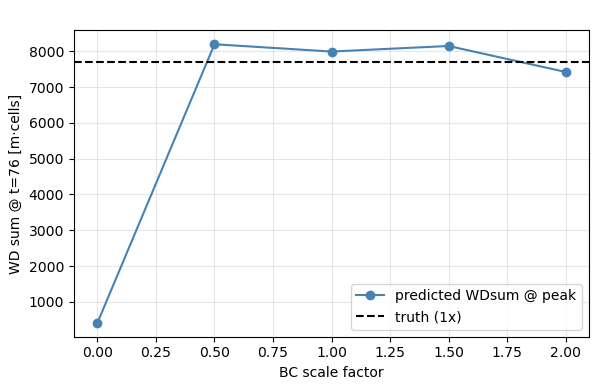
\includegraphics[width=0.8\textwidth]{total_water_volumeVSscalers.png}
  \caption{Magnitude-scaling test, single-simulation reference model. Predicted water-depth sum at
    the flood peak ($t=76$); the dashed line is the water-depth sum of the actual 1$\times$
    case-study simulation itself, shown as a fixed reference .}
  \label{fig:forcing-singlesim}
\end{figure}
 
Figure~\ref{fig:forcing-singlesim} confirms the on/off pattern anticipated in
Section~\ref{subsec:hyperparam_loss}: CSI@0.05 collapses only at zero forcing (0.638)
and is otherwise flat and non-monotonic across the full 0.5--2.0$\times$ range
(0.711--0.741). As soon as any non-zero forcing is applied,
then stays close to the training case study level regardless of the scale factor rather than
tracking it. 
This is clear evidence that the single-simulation model has learned
to reproduce the training event rather than to model the underlying flood process, and
motivates the multi-simulation training of the following sections.
 
\section{Four-Simulation Model}
\label{sec:res_four_sim}
 
\subsection{Accuracy on Held-Out Magnitude}
\label{subsec:res_four_sim_accuracy}
 
The four-simulation model (trained on the 2021 event scaled by
0.5$\times$/0.75$\times$/1.25$\times$/1.5$\times$, Section~\ref{subsec:multisimtraining})
is evaluated on the unscaled (1$\times$) event, held out entirely from training. Unlike
the single-simulation numbers of Section~\ref{sec:res_single_sim}, these metrics
therefore measure generalisation to unseen forcing, not reproduction.
 
\begin{table}[H]
  \centering
  \caption{Four-simulation model accuracy on the held-out 1$\times$ event (best val.\
    loss checkpoint, epoch 813).}
  \label{tab:foursim-accuracy}
  \begin{tabular}{ccc}
    \toprule
    RMSE WD [m] & CSI@0.05 & CSI@0.30 \\
    \midrule
    0.130 & 0.799 & 0.852 \\
    \bottomrule
  \end{tabular}
\end{table}
 
Table~\ref{tab:foursim-accuracy} can be compared directly against the single-simulation
reference model of Section~\ref{subsec:res_single_sim_accuracy}
(RMSE~$=0.158$~m, CSI@0.05~$=0.775$, CSI@0.30~$=0.832$,
Table~\ref{tab:multiscale-loss}). The four-simulation model improves on every metric, despite being evaluated on a harder task (generalization on an event held out from training). Training on more simulations therefore genuinely improves the model's
accuracy on unseen forcing.
 
\subsection{Magnitude-Scaling Sensitivity}
\label{subsec:res_four_sim_magnitude_sensitivity}
 
 
\begin{figure}[H]
  \centering
  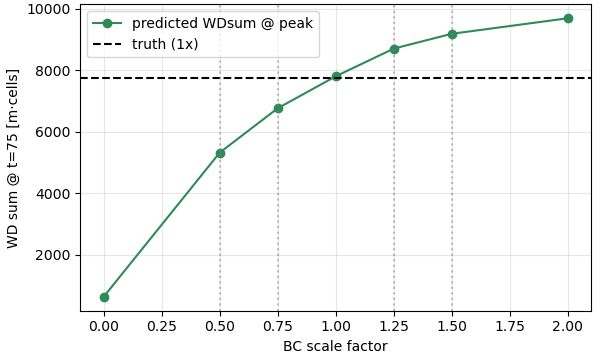
\includegraphics[width=0.8\textwidth]{multisim_total_water_volumeVSscalers.png}
  \caption{Magnitude-scaling test, four-simulation model.
    Predicted water-depth sum at the flood peak
    ($t=75$); the dashed line is the water-depth sum of the actual 1$\times$
    case-study simulation, and the dotted vertical lines mark the four scale factors
    (0.5, 0.75, 1.25, 1.5$\times$) seen during training.}
  \label{fig:forcing-foursim}
\end{figure}
 
Figure~\ref{fig:forcing-foursim} resolves the single-simulation model's flat response:
WD-sum at peak now increases closely to monotonically with BC scale factor across the
full tested range . $0.5\times$,
$0.75\times$, $1.25\times$, and $1.5\times$ were seen during training; $0\times$,
$1\times$, and $2\times$ were not. So the smooth response through $1\times$, and the
graceful degradation at $2\times$, are both genuine interpolation/extrapolation
behaviour. Table~\ref{tab:foursim-extrapolation} extends
the $2\times$/$3\times$ end of this test further with dedicated held-out SFINCS
simulations.
 
 
 
\begin{table}[H]
  \centering
  \caption{Extrapolation beyond the training magnitude range, four-simulation model,
    evaluated on dedicated held-out 2$\times$/3$\times$ SFINCS simulations.}
  \label{tab:foursim-extrapolation}
  \begin{tabular}{lccc}
    \toprule
    Scale & RMSE WD [m] & CSI@0.05 & CSI@0.30 \\
    \midrule
    1.0$\times$ (context) & 0.130 & 0.799 & 0.852 \\
    2.0$\times$            & 0.220 & 0.794 & 0.851 \\
    3.0$\times$            & 0.379 & 0.775 & 0.828 \\
    \bottomrule
  \end{tabular}
\end{table}
 
Degradation with increasing extrapolation distance is gradual: CSI@0.05
falls by only 0.024 from 1$\times$ to 3$\times$, while RMSE roughly triples, reflecting
error growth concentrated in peak-depth magnitude rather than in flood-extent
classification.
 
\subsection{Non-Uniform Forcing Sensitivity}
\label{subsec:res_four_sim_sensitivity}
 
The non-uniform forcing test of Section~\ref{sec:physics_sensitivity_method} isolates
whether the model attends to \emph{which} source location an inflow enters at, rather
than only to the total forcing magnitude tested in
Section~\ref{subsec:res_four_sim_magnitude_sensitivity}. Two source groupings are tested: the main stem
(Kirmutscheid, 49.8\% of total forcing volume) and the three smallest tributaries
combined (new1, Niederadenau, new2; 18.5\% of total forcing volume). Kreuzberg,
Denn, and Muesch are held at 1$\times$ throughout.
Dedicated SFINCS simulations were run for all seven scenarios, so each is judged
against its own "true outcome".
 
\begin{table}[H]
  \centering
  \caption{Non-uniform BC sensitivity test, four-simulation model, each scenario against its own dedicated SFINCS ground truth.
    ``Lag'' is the model's peak-timing error in hours (positive = predicted peak
    arrives late).}
  \label{tab:foursim-blockbc}
  \resizebox{\textwidth}{!}{%
  \begin{tabular}{lcccccc}
    \toprule
    Scenario & Lag [h] & Real peak & Pred peak & RMSE WD [m] & CSI@0.05 & CSI@0.30 \\
    \midrule
    Baseline (1$\times$)             & $+1$  & 7767 & 7919 & 0.132 & 0.796 & 0.847 \\
    Tributaries $\to 0\times$        & $-1$  & 6650 & 7349 & 0.144 & 0.785 & 0.836 \\
    Tributaries $\to 2\times$        & $+1$  & 8920 & 8775 & 0.159 & 0.790 & 0.841 \\
    Main stem $\to 0\times$          & $0$   & 5059 & 7687 & 0.179 & 0.743 & 0.743 \\
    Main stem $\to 2\times$          & $+1$  & 9976 & 8139 & 0.205 & 0.795 & 0.838 \\
    Only main stem active            & $-10$ & 5270 & 2203 & 0.207 & 0.719 & 0.727 \\
    Only smallest tributary active   & $+1$  & 842  & 4898 & 0.205 & 0.570 & 0.506 \\
    \bottomrule
  \end{tabular}%
  }
\end{table}
 
Table~\ref{tab:foursim-blockbc} shows three patterns:
 
Timing is
accurate almost everywhere: every scenario's predicted flood peak lands within
$\pm 1$~h of the real one, except main-stem-only, where the prediction peaks
10~h too early. 
 
Magnitude response is directionally correct but severely
damped for the main stem specifically. Removing the main stem entirely drops the real
peak by 34.9\% (7767~$\to$~5059), but the corresponding prediction barely moves
(7919~$\to$~7687, a 2.9\% drop): the model captures less than a tenth of the true
sensitivity to losing its largest single source. Doubling the main stem shows the same
pattern in reverse, a real increase of 28.4\% predicted as only 2.8\%. The three
smallest tributaries combined, despite representing barely a third of the main stem's
volume, are tracked with visibly better magnitude fidelity (real $-14.4\%$ predicted
as $-7.2\%$; real $+14.8\%$ predicted as $+10.8\%$). 
 
The two isolation
scenarios fail in opposite directions. With only the main stem active, the model
under-predicts badly (real 5270, predicted 2203, and the 10~h timing error above);
with only the smallest tributary active, it over-predicts even more badly (real 842,
essentially no flood, predicted 4898, a substantial one). Taken together, these results describe a model that is least reliable when the forcing configuration departs furthest from the training distribution's default of all seven sources active together.
 
The leave-one-out ladder (Table~\ref{tab:foursim-ladder}) adds a further, sharper example of the same
volume-independence: Kreuzberg, only 8.5\% of total forcing volume, produces the
largest single-location sensitivity in the entire ladder ($-48.6\%$ peak WD-sum when
zeroed), more than fifteen times the effect of zeroing the main stem itself ($-3.2\%$). Every other location, including the main stem, falls in a
comparatively narrow $-0.2\%$ to $-5.5\%$ band regardless of its own volume share.
 
Kirmutscheid enters at the far upstream end of the river course, well removed from
the Altenahr--Bad Neuenahr-Ahrweiler gorge where peak water depths concentrated
(Section~\ref{subsec:ahr_basin}); Kreuzberg enters much closer to that reach. A
response organised by spatial proximity to peak water depth, rather than by forcing
volume, would produce exactly the localised pattern Table~\ref{tab:foursim-ladder}
shows: the model appears not to have learned each source's weight within the flood
as a whole, and instead confines a perturbation's effect to the area local to that
inflow point.
Flood maps at the peak timestep for
each scenario, which would let this hypothesis be checked directly, are provided in
the Appendix~\ref{app:nonuniform_maps_foursim}.
 
\begin{table}[H]
  \centering
  \caption{Per-location leave-one-out sensitivity ladder, four-simulation model, against the actual 1$\times$ case-study simulation.
    Sorted by volume share, descending.}
  \label{tab:foursim-ladder}
  \begin{tabular}{lccccc}
    \toprule
    Location & Vol.\ share & $\Delta$peak (0$\times$) & $\Delta$peak (2$\times$)  \\
    \midrule
    Kirmutscheid (main stem) & 49.8\% & $-3.2\%$  & $+2.6\%$  \\
    Muesch                   & 12.7\% & $-3.7\%$  & $+3.5\%$  \\
    Denn                     & 10.6\% & $-5.5\%$  & $+3.7\%$ \\
    Kreuzberg                & 8.5\%  & $-48.6\%$ & $+12.3\%$ \\
    Niederadenau              & 7.5\%  & $-0.2\%$  & $+0.6\%$ \\
    new1                     & 7.4\%  & $-2.3\%$  & $+3.1\%$ \\
    new2 (smallest)          & 3.6\%  & $-1.5\%$  & $+7.9\%$ \\
    \bottomrule
  \end{tabular}
\end{table}
 
The four-simulation model's recession behaviour is a genuine limitation: the
held-out, post-peak catchment-emptying scenario (draining from the flood peak with
all discharge set to zero) shows the real SFINCS event drains to 1.9\% of its
initial volume by the end of the record, while the model's prediction retains
39.6\%, more than twenty times too much water (RMSE~$=0.267$~m, CSI@0.05~$=0.200$). 

%A held-out, direction-flipped timing
%desynchronisation scenario (every
%tributary's timing offset shifted, in a direction never seen in training) fares
%better but still shows a real generalisation gap, not just noise: CSI@0.05 drops from
%0.796 in-distribution to 0.762 (RMSE~$=0.252$~m). 
%maybe not too central, would move to the annexes
 
\subsection{Sensitivity to the Ungauged-Tributary Reconstruction Method}
\label{subsec:res_four_sim_bc_method}
 
Because three of the seven inflow locations have no discharge record and were
reconstructed (Section~\ref{subsec:ungauged}), the sensitivity of the model's
prediction to which reconstruction method was used needs to be checked. Three
datasets are compared: the area-weighted residual method used for
training throughout this thesis (Method 1, Section~\ref{subsubsec:method1}), the
rainfall-weighted residual with Kirpich routing lag (Method 2,
Section~\ref{subsubsec:method2}), and the SCS-CN method with a triangular unit
hydrograph (Method 3, Section~\ref{subsubsec:method3}). All three datasets share the
same gauged forcing, warm start, and domain; only the three ungauged-tributary
hydrographs differ.
 
\begin{table}[H]
  \centering
  \caption{Four-simulation model accuracy under the three ungauged-tributary
    reconstruction methods, each evaluated against its own method-specific ground
    truth.}
  \label{tab:bcmethod-accuracy}
  \begin{tabular}{lccc}
    \toprule
    Reconstruction method & RMSE WD [m] & CSI@0.05 & CSI@0.30 \\
    \midrule
    Method 1 (area-weighted)                    & 0.130 & 0.799 & 0.852 \\
    Method 2 (rainfall-weighted, Kirpich)  & 0.153 & 0.792 & 0.843 \\
    Method 3 (SCS-CN, unit hydrograph)     & 0.147 & 0.784 & 0.837 \\
    \midrule
    Spread (mean $\pm$ std, $n=3$)          & $0.144 \pm 0.012$ & $0.792 \pm 0.008$ & $0.844 \pm 0.007$ \\
    \bottomrule
  \end{tabular}
\end{table}
 
The spread across reconstruction methods is comparable in magnitude to the
seed-to-seed training-randomness spread of Table~\ref{tab:seed-ruler}: RMSE
$0.144 \pm 0.012$ against the reference band's
$0.142 \pm 0.010$, with the two
ranges almost fully overlapping. On RMSE, not knowing the true ungauged-tributary
discharge is therefore not clearly separable from ordinary re-training noise. CSI@0.05
tells a more favourable story on its own ($0.792 \pm 0.008$ against the reference band's
$0.761 \pm 0.042$, a much narrower spread).
 
This comparison also tests whether the model amplifies or smooths over the
input-forcing disagreement between methods, by comparing the RMSE between each pair of
methods' own SFINCS ground truths (how different the real floods actually are) against
the RMSE between the model's corresponding predictions (Table~\ref{tab:bcmethod-amplification}).
 
\begin{table}[H]
  \centering
  \caption{Ground-truth disagreement vs.\ predicted disagreement between each pair of
    reconstruction methods. A ratio near 1 indicates the model propagates the input
    disagreement faithfully; a ratio above 1 indicates amplification.}
  \label{tab:bcmethod-amplification}
  \begin{tabular}{lccc}
    \toprule
    Method pair & Truth-vs-truth RMSE & Pred-vs-pred RMSE & Ratio \\
    \midrule
    Method 1 vs.\ Method 2 & 0.084 & 0.082 & 0.98 \\
    Method 1 vs.\ Method 3 & 0.050 & 0.090 & 1.78 \\
    Method 2 vs.\ Method 3 & 0.052 & 0.085 & 1.64 \\
    \bottomrule
  \end{tabular}
\end{table}
 
The model reproduces the Method 1-vs-Method-2 disagreement almost exactly (ratio
0.98), but nearly doubles the disagreement for any comparison involving Method 3
(ratios 1.64--1.78).
For Method 3 the model overshoots this disagreement somewhat, though not
dramatically, so its behaviour here can still be considered reasonable overall.
 
 
\section{Twenty-Simulation Model}
\label{sec:res_twenty_sim}
 
The twenty-simulation model (Section~\ref{subsec:multisimtraining}) was trained under
the same reference configuration and evaluated on the same held-out 1$\times$ event.
 
\begin{table}[H]
  \centering
  \caption{Twenty-simulation model accuracy on the held-out 1$\times$ event, against the four-simulation and single-simulation reference models.}
  \label{tab:twentysim-accuracy}
  \begin{tabular}{lccc}
    \toprule
    Configuration & RMSE WD [m] & CSI@0.05 & CSI@0.30 \\
    \midrule
    20-sim                     & 0.101 & 0.853 & 0.899 \\
    4-sim (reference)          & 0.130 & 0.799 & 0.852 \\
    1-sim (reference, training event) & 0.158 & 0.775 & 0.832 \\
    \bottomrule
  \end{tabular}
\end{table}
 
The twenty-simulation model improves on every metric relative to both the
four-simulation model (Section~\ref{subsec:res_four_sim_accuracy}) and the
single-simulation reference (Section~\ref{subsec:res_single_sim_accuracy}), despite
being evaluated, like the four-simulation model, on an event held out entirely from
training rather than on the training event itself. The same increase in training diversity that helped the
four-simulation model over the single-simulation one continues to help at twenty
simulations.
 
\subsection{Magnitude-Scaling Sensitivity}
\label{subsec:res_twenty_sim_magnitude_sensitivity}
 
The magnitude response follows the same monotonic-WD-sum pattern established by the
four-simulation model (Section~\ref{subsec:res_four_sim_magnitude_sensitivity}).
 
 
\subsection{Non-Uniform Forcing and Compositional Generalisation}
\label{subsec:res_twenty_sim_nonuniform}
 
The twenty-simulation training set (Section~\ref{subsec:multisimtraining}) directly
includes per-tributary magnitude perturbations, a timing shift of the dominant
tributary, one all-locations-desynchronised event, and one catchment-emptying event.
The tests in this section therefore check generalisation to \emph{new combinations} of
scale, lag, and tributary grouping, not to entirely unfamiliar kinds of perturbation.
 
\paragraph{Fixed: per-location weighting.}
The per-location leave-one-out ladder (Table~\ref{tab:twentysim-ladder}) no longer shows the
four-simulation model's extreme, volume-independent outlier (Kreuzberg, $-48.6\%$ from
8.5\% of volume, Table~\ref{tab:foursim-ladder}). Kirmutscheid, the main stem and
49.8\% of total forcing volume, now produces the \emph{largest} single-location
response in the ladder ($-23.8\%$ peak WD-sum when zeroed), and the ranking of
response magnitude broadly tracks volume share. Kreuzberg remains somewhat ahead of its volume share, but by a
factor of roughly two rather than the order-of-magnitude seen in the four-simulation
model. 
 
This improvement is best read as the model actually learning each
tributary's contribution to the flood, rather than continuing to respond only to
whatever is local to each inflow point (Section~\ref{subsec:res_four_sim_sensitivity}).
 
\begin{table}[H]
  \centering
  \caption{Per-location leave-one-out sensitivity ladder, twenty-simulation model, against the actual 1$\times$ case-study simulation.
    Sorted by volume share, descending.}
  \label{tab:twentysim-ladder}
  \begin{tabular}{cccc}
    \toprule
    Location & Vol.\ share & $\Delta$peak (0$\times$) & $\Delta$peak (2$\times$) \\
    \midrule
    Kirmutscheid (main stem) & 49.8\% & $-23.8\%$ & $+14.1\%$ \\
    Muesch                   & 12.7\% & $-10.8\%$ & $+4.5\%$ \\
    Denn                     & 10.6\% & $-12.4\%$ & $+2.1\%$ \\
    Kreuzberg                & 8.5\%  & $-18.0\%$ & $+5.7\%$  \\
    Niederadenau              & 7.5\%  & $-7.8\%$  & $+4.2\%$\\
    new1                     & 7.4\%  & $-5.1\%$  & $+4.7\%$ \\
    new2 (smallest)          & 3.6\%  & $-5.6\%$  & $+4.2\%$ \\
    \bottomrule
  \end{tabular}
\end{table}
 
 
\begin{table}[H]
  \centering
  \caption{Non-uniform BC sensitivity test, twenty-simulation model, each scenario against its own dedicated SFINCS ground truth. Same
    scenario definitions as Table~\ref{tab:foursim-blockbc}.}
  \label{tab:twentysim-blockbc}
  \resizebox{\textwidth}{!}{%
  \begin{tabular}{lcccccc}
    \toprule
    Scenario & Lag [h] & Real peak & Pred peak & RMSE WD [m] & CSI@0.05 & CSI@0.30 \\
    \midrule
    Baseline (1$\times$)             & $0$  & 7767 & 8940  & 0.129 & 0.833 & 0.882 \\
    Tributaries $\to 0\times$        & $-1$ & 6650 & 7555  & 0.119 & 0.833 & 0.884 \\
    Tributaries $\to 2\times$        & $0$  & 8920 & 9356  & 0.143 & 0.829 & 0.878 \\
    Main stem $\to 0\times$          & $0$  & 5059 & 6305  & 0.129 & 0.810 & 0.795 \\
    Main stem $\to 2\times$          & $0$  & 9976 & 10064 & 0.151 & 0.824 & 0.886 \\
    Only main stem active            & $+1$ & 5270 & 5875  & 0.124 & 0.817 & 0.836 \\
    Only smallest tributary active   & $-3$ & 842  & 3195  & 0.154 & 0.624 & 0.540 \\
    \bottomrule
  \end{tabular}%
  }
\end{table}
 
 \textbf{Timing is now tightly controlled}: lag ranges from
$-3$~h to $+1$~h across all seven scenarios. 
 
\textbf{Main-stem magnitude accuracy improves sharply}: the peak error for
zeroing the main stem falls from $+51.9\%$ to $+24.6\%$, for doubling it falls from
$-18.4\%$ to $+0.9\%$, and for the main-stem-only isolation scenario falls from
$-58.2\%$ (a severe under-prediction) to $+11.5\%$ (a modest over-prediction): the
same scenario that carried the $-10$~h timing failure in the four-simulation model is
now both correctly timed and reasonably sized.
 
\textbf{The smallest-tributary-only
isolation scenario remains the weak point}: peak error falls from $+481.9\%$
to $+279.6\%$, a real improvement, but still by far the largest error in the table. With almost the entire catchment's
forcing switched off and only the smallest tributary active, the model still predicts
a substantially larger flood than SFINCS produces.
 
 
 
\paragraph{Fixed: timing generalisation.}
The held-out, direction-flipped timing desynchronisation scenario (every tributary's
timing offset shifted, in a direction never seen in training) performs close to the
SFINCS ground truth of that same event: CSI@0.05~$=0.818$, CSI@0.30~$=0.865$,
RMSE~$=0.145$~m. Given that the training set
already includes one all-locations-desynchronisation event, with different
offsets, this is consistent with the model having learned each tributary's timing
contribution well enough to interpolate to a related but unseen combination.
 
\paragraph{Not fixed: drainage and long-horizon recession.}
Two results together point to the same underlying failure: the model has learned the
generic temporal shape of the $\sim$118--120-step training simulations, rise followed
by partial recession.
 
On the held-out post-peak draining scenario, the predicted total water depth does
initially decrease after the peak, consistent with the recession the model has seen
many times in training. But once the rollout continues past roughly the
$\sim$118--120-step horizon common to nineteen of the twenty training simulations,
rather than continuing to drain toward zero, the prediction settles and then slightly
increases again (Figure~\ref{fig:twentysim-emptying-wdsum}).
 
\begin{figure}[H]
  \centering
  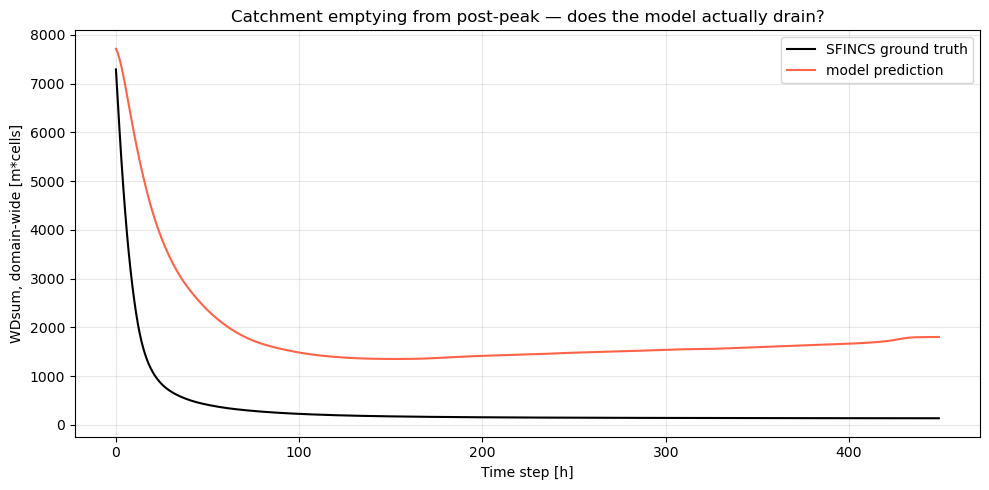
\includegraphics[width=0.8\textwidth]{emptying_from_peak_20sim.png}
  \caption{Domain-wide water-depth sum over the full rollout, held-out post-peak
    catchment-emptying scenario, twenty-simulation model.}
  \label{fig:twentysim-emptying-wdsum}
\end{figure}
 
On the in-training-set catchment-emptying scenario (from the pre-event baseline), the
predicted total water depth \emph{increases} over time despite the complete absence of
forcing, because rising water is what every other training simulation does
near $t=0$, and this one scenario's forcing is enough to override that
learned default.
 
Because this second scenario \emph{is} in the training set, the failure cannot be
attributed to compositional generalisation. The most likely explanation is data
density: nineteen of the twenty training
simulations end at the same $\sim$118--120-step event horizon and never show a full
drain, so with only one draining example to learn from, the model has learned what a
typical rollout looks like far more reliably than it has learned to override that
default when the forcing actually calls for it. This thesis's focus is the flood event
itself, rather than long-term catchment
drainage, so this limitation was not prioritised for a fix; the direct
remedy, extending every training simulation to full drainage rather than stopping near
the event horizon, is left as a recommendation for future work.

 
\section{False-Positive Over-Wetting as the Dominant Error Mode}
\label{sec:res_fp_overwetting}

Decomposing rollout error into false positives
(predicted wet, actually dry) and false negatives (predicted dry, actually wet)
shows over-wetting is consistently the dominant failure
mode across every model generation (Table~\ref{tab:fp-dominance}), and it was
substantially worse before the multiscale loss was adopted.

\begin{table}[H]
    \centering
    \caption{Mean FP/wet and FN/wet ratios (water
      depth threshold 0.05~m) across the model progression.}
    \label{tab:fp-dominance}
    \begin{tabular}{lccl}
        \toprule
        Configuration & Mean FP/wet & Mean FN/wet & Dominant error \\
        \midrule
        Single-sim, finest-scale loss only & 0.445 & 0.044 & FP (over-wetting) \\
        Single-sim, multiscale loss                          & 0.255 & 0.052 & FP (over-wetting) \\
        Four-sim, multiscale loss                            & 0.209 & 0.042 & FP (over-wetting) \\
        Twenty-sim, multiscale loss                           & 0.150 & 0.026 & FP (over-wetting) \\
        \bottomrule
    \end{tabular}
\end{table}

FP dominates at every point in the progression, and each of the two
interventions made elsewhere in this thesis reduces it independently: adopting
multiscale loss alone, holding training data fixed at one simulation, nearly
halves the ratio (0.445 to 0.255); scaling from one to twenty training
simulations, holding the loss configuration fixed, halves it again
(0.255 to 0.150). Over-wetting is therefore a genuine, persistent limitation but both design choices
already adopted in this thesis address it in part.

Figure~\ref{fig:fp-overwetting-maps} shows where these false alarms sit, side by
side across all four models in Table~\ref{tab:fp-dominance}, at the flood peak
of the same $1\times$ event: scattered, off-channel red cells rather
than a fringe around the true flood extent, visibly denser for the
pre-multiscale single-simulation model than for the twenty-simulation model,
but present in every panel.

\begin{figure}[H]
    \centering
    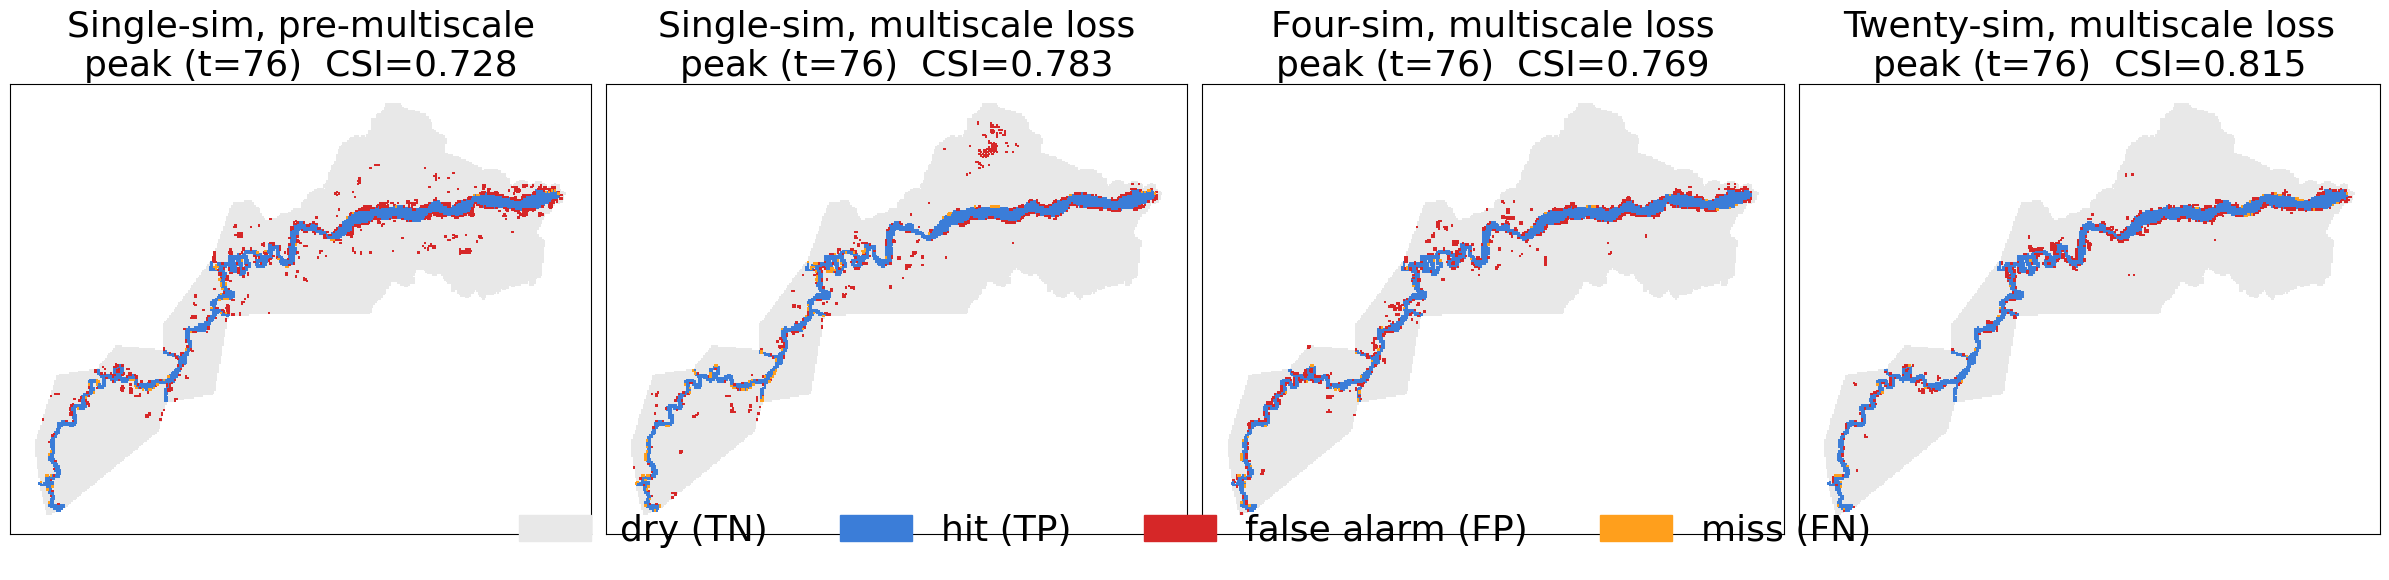
\includegraphics[width=\textwidth]{FP_overview_different_models.png}
    \caption{Hit/false-alarm/miss classification at the flood peak, for the
      four models of Table~\ref{tab:fp-dominance}: single-simulation
      pre-multiscale loss, single-simulation with multiscale loss,
      four-simulation, and twenty-simulation, on the same $1\times$ event.}
    \label{fig:fp-overwetting-maps}
\end{figure}

This is a genuine limitation, not addressed here (Section~\ref{sec:limitations_future_work}).

 
\section{Hydraulic Structure Representation}
\label{sec:res_structures}
 
The structure-aware model (Section~\ref{sec:structure_scenarios}) is retrained on the
32-event merged dataset (the twenty BC-augmentation events plus twelve levee/dam
structure scenarios) and compared throughout this section
against the twenty-simulation model of Section~\ref{sec:res_twenty_sim}, which never
saw a structure scenario, in order to isolate what structure-awareness itself changes.
 
\subsection{Accuracy on the Core Flood Event}
\label{subsec:res_structures_core_accuracy}
 
On the standard held-out 1$\times$ event, which contains no structures, the
structure-aware model is modestly worse than the twenty-simulation
model: RMSE~$=0.112$~m against $0.101$~m, CSI@0.05~$=0.810$ against $0.853$,
CSI@0.30~$=0.877$ against $0.899$. Training on the additional, structurally very different
levee/flow obstruction scenarios appears to cost a small amount of accuracy and calibration on the
core flood event (multi-task trade-off).
 
\subsection{Why Is Retraining Necessary?}
\label{subsec:res_structures_sanity}
 
Structures are represented as an additional edge feature (Section~\ref{subsubsec:structures_gnn}), so $\texttt{edge\_attr}$ grows from one dimension (length) to
two (length and crest height).
Since the edge encoder's input dimensionality is fixed at training time, only a model
trained with both features can read a crest value at all: a model trained on the
original, one-feature representation has no mechanism to consume it, regardless of
whether the value is present in the input data. This is why the structure-aware model
had to be retrained from scratch (Section~\ref{sec:structure_scenarios}) rather than
simply evaluating an existing checkpoint on structure scenarios.
 
The twenty-simulation model illustrates the consequence directly, and doubles as a
lower bound for what follows: it can only ever see edge length, so evaluating it on
the structure-scenario dataset is equivalent to testing it on a new,
slightly different mesh, since the structure-constrained triangulation
(Section~\ref{subsubsec:structures_gnn}) changes edge lengths across the mesh. Its accuracy collapses relative to its own core-event
performance (Section~\ref{sec:res_twenty_sim}): RMSE rises from $0.101$~m to
$0.55$--$0.65$~m and CSI@0.05 falls from $0.853$ to $0.55$--$0.62$ across the four
held-out scenarios (Table~\ref{tab:structures-heldout}). Figure~\ref{fig:bcaugment-chaos}
shows why: false alarms are not confined to the area near the structure, which is
roughly what a model only missing that one local effect might produce, but scattered
widely across the domain, consistent with a more general mesh mismatch rather than a
narrowly localised gap.
 
\begin{figure}[H]
  \centering
  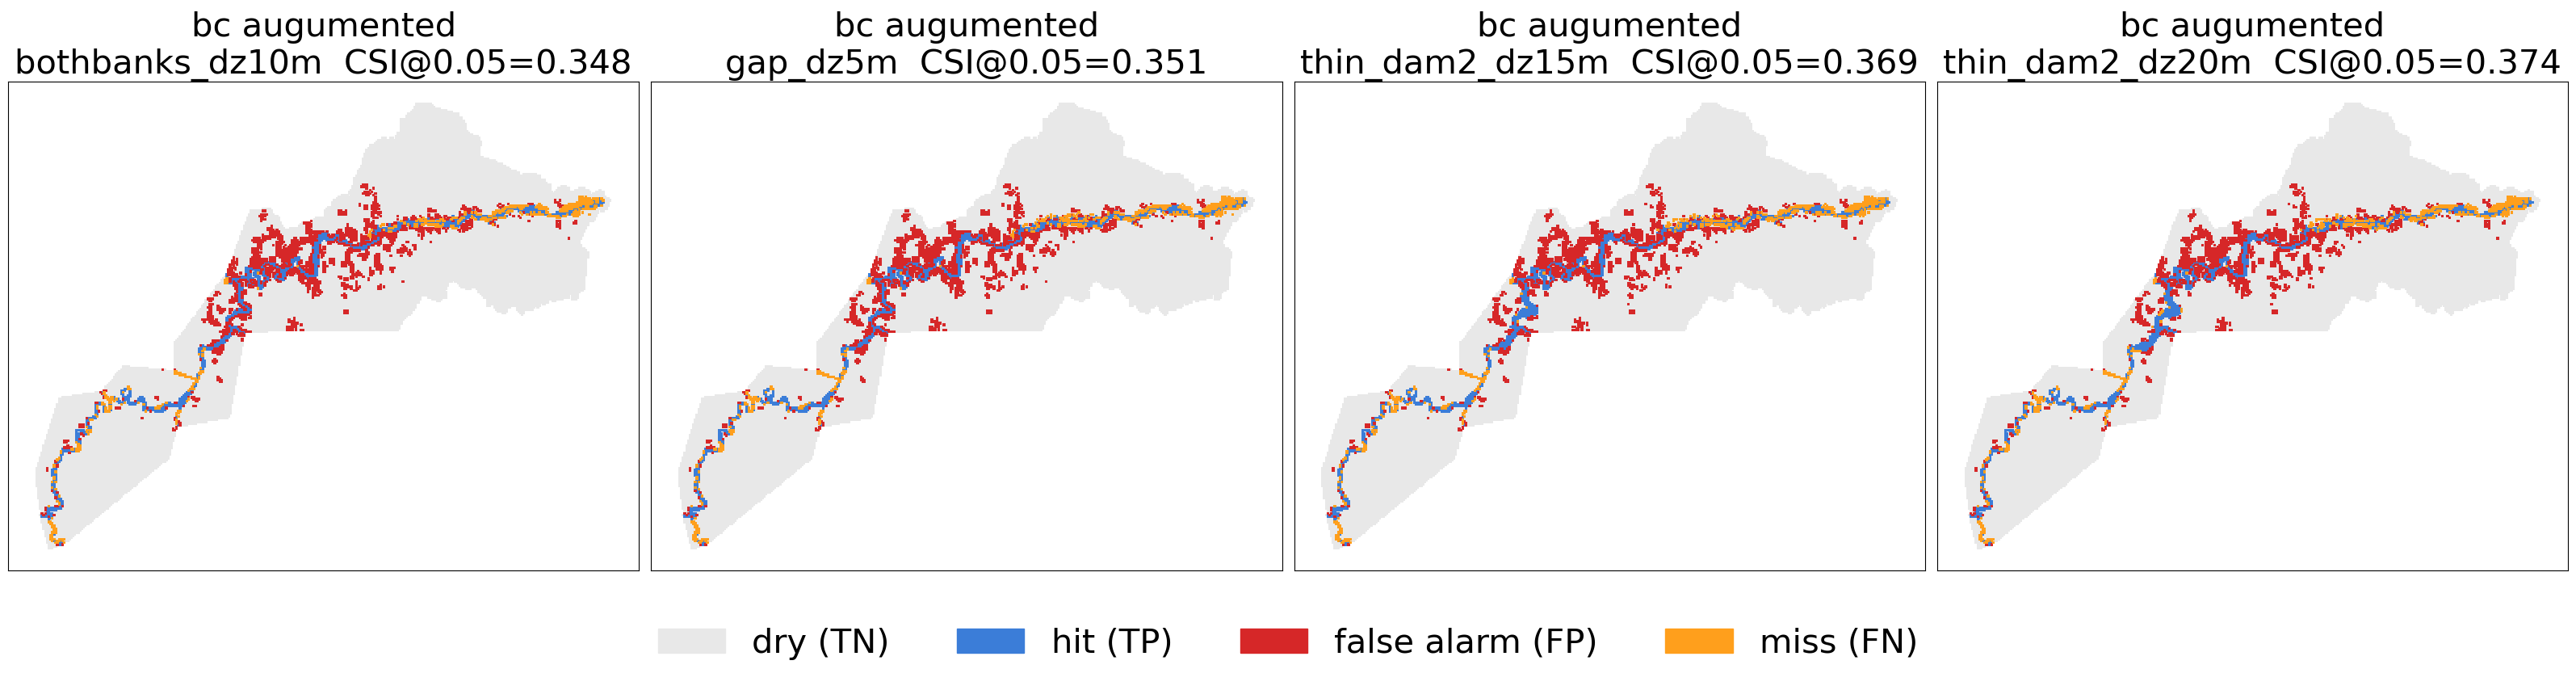
\includegraphics[width=1\textwidth]{bc_augumented_caos.png}
  \caption{Spatial hit/false-alarm/miss classification at the final timestep, twenty-simulation
    model (no structures) on the four held-out structure scenarios.}
  \label{fig:bcaugment-chaos}
\end{figure}
 
A plausible reading is that the twenty-simulation model has, in effect, overfit to
the specific edge-length statistics of its own training mesh, so an
out-of-distribution mesh geometry degrades its predictions well beyond what simply
lacking the crest information would.
 
 
\subsection{Generalisation to Held-Out Structure Configurations}
\label{subsec:res_structures_generalisation}
 
Four scenarios were held out entirely from the structure-aware model's training set
(Section~\ref{sec:structure_scenarios}), each testing a different generalisation axis:
an unseen magnitude (a levee crest twice as high as the highest one trained on), an
unseen structural footprint (a breach in an otherwise-trained levee configuration),
and an unseen locations for the flow obstruction mechanism ($\sim$3--4~km from the trained
crossing, at both trained crest heights).
 
\begin{table}[H]
  \centering
  \caption{Held-out structure-scenario generalisation, structure-aware model vs.\ the
    twenty-simulation model (no structures), each against
    its own dedicated SFINCS ground truth.}
  \label{tab:structures-heldout}
  \resizebox{\textwidth}{!}{%
  \begin{tabular}{llccc}
    \toprule
   Scenario & Model & RMSE WD [m] & CSI@0.05 & CSI@0.30 \\
    \midrule
    Levee, unseen magnitude (both banks, $+10$~m) & Structure-aware & 0.119 & 0.799 & 0.866 \\
    Levee, unseen magnitude (both banks, $+10$~m) & No structures   & 0.549 & 0.619 & 0.660 \\
    \addlinespace
    Levee, unseen footprint (breach, $+5$~m)      & Structure-aware & 0.120 & 0.799 & 0.864 \\
    Levee, unseen footprint (breach, $+5$~m)      & No structures   & 0.550 & 0.620 & 0.658 \\
    \addlinespace
    flow obstruction, unseen location, crest $+15$~m       & Structure-aware & 0.298 & 0.769 & 0.713 \\
    flow obstruction, unseen location, crest $+15$~m       & No structures   & 0.607 & 0.602 & 0.534 \\
    \addlinespace
    flow obstruction, unseen location, crest $+20$~m       & Structure-aware & 0.384 & 0.764 & 0.706 \\
    flow obstruction, unseen location, crest $+20$~m       & No structures   & 0.650 & 0.602 & 0.536 \\
    \bottomrule
  \end{tabular}%
  }
\end{table}
 
The two generalisation axes are not equally well handled, however.
The unseen-magnitude and unseen-footprint levee scenarios reach RMSE~$\approx 0.12$~m
and CSI@0.05~$\approx 0.80$, close to the core-event accuracy of
Section~\ref{subsec:res_structures_core_accuracy}. The unseen-location thin-dam
scenarios are markedly worse, RMSE $0.30$--$0.38$~m and CSI@0.05~$\approx 0.77$.
Figure~\ref{fig:levee-zoom} shows the levee case directly, zoomed
to the affected reach. Without a structure, the flood spreads diffusely beyond the
channel, with visible patches of inundation on the floodplain either side of the
main flow path. With the $+10$~m levee in place, SFINCS's own ground truth shows the
flood visibly narrowed and confined along the channel between the two banks. The
structure-aware model's prediction moves in the same direction, but the containment
is not as clean as SFINCS's own: scattered patches of water remain outside the
leveed channel where the ground truth shows none, most visibly towards the right of
the reach. The model has clearly learned that the levee changes the flood, but has
not learned to confine it as strictly as SFINCS does.
This scenario tests extrapolation specifically: a $+10$~m crest is twice the highest
levee height seen during training. The same pattern already established for the
twenty-simulation model's own physical-consistency checks
(Section~\ref{subsec:res_structures_sensitivity}) applies here too, accuracy degrades
gracefully but steadily the further a scenario sits from the training range, and it
extends naturally to a structure's own magnitude. The model has learned that a levee reduces the flood, but has not learned
to scale that reduction proportionally with crest height, plausibly because the
twelve training scenarios represent the levee too sparsely to pin the relationship
down precisely.
 
 
\begin{figure}[H]
  \centering
  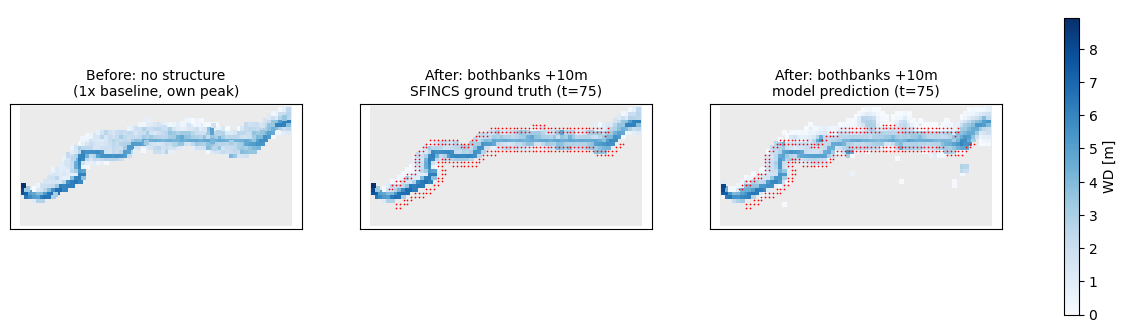
\includegraphics[width=1\textwidth]{thin_dam_10m.png}
  \caption{Levee effect at Bad Neuenahr-Ahrweiler. Left: no structure (standard 1$\times$ event).
    Centre: SFINCS ground truth with a $+10$~m levee on both banks (held-out crest
    height). Right: the structure-aware model's prediction of the same scenario. Red
    markers indicate the nodes adjacent to a tagged structure edge.}
  \label{fig:levee-zoom}
\end{figure}
 
\subsection{The Levee/flow obstruction Asymmetry}
\label{subsec:res_structures_asymmetry}
 
Whether the flow obstruction gap above is a generalisation shortfall or a harder problem with the flow obstruction mechanism itself, can be
checked directly: two of the twelve training scenarios are flow obstruction crossings at the
trained location, so their accuracy is not a generalisation question. If
training had worked cleanly, these in-training-set scenarios should look close to the
core-event. They do not: RMSE~$0.25$~m
(crest~$+15$~m) and $0.32$~m (crest~$+20$~m), CSI@0.05~$\approx 0.73$
(Figure~\ref{fig:thindam-training-fail}). The flow obstruction mechanism is therefore
harder for the model throughout, independent of whether the specific configuration
was seen during training.
 
\begin{figure}[H]
  \centering
  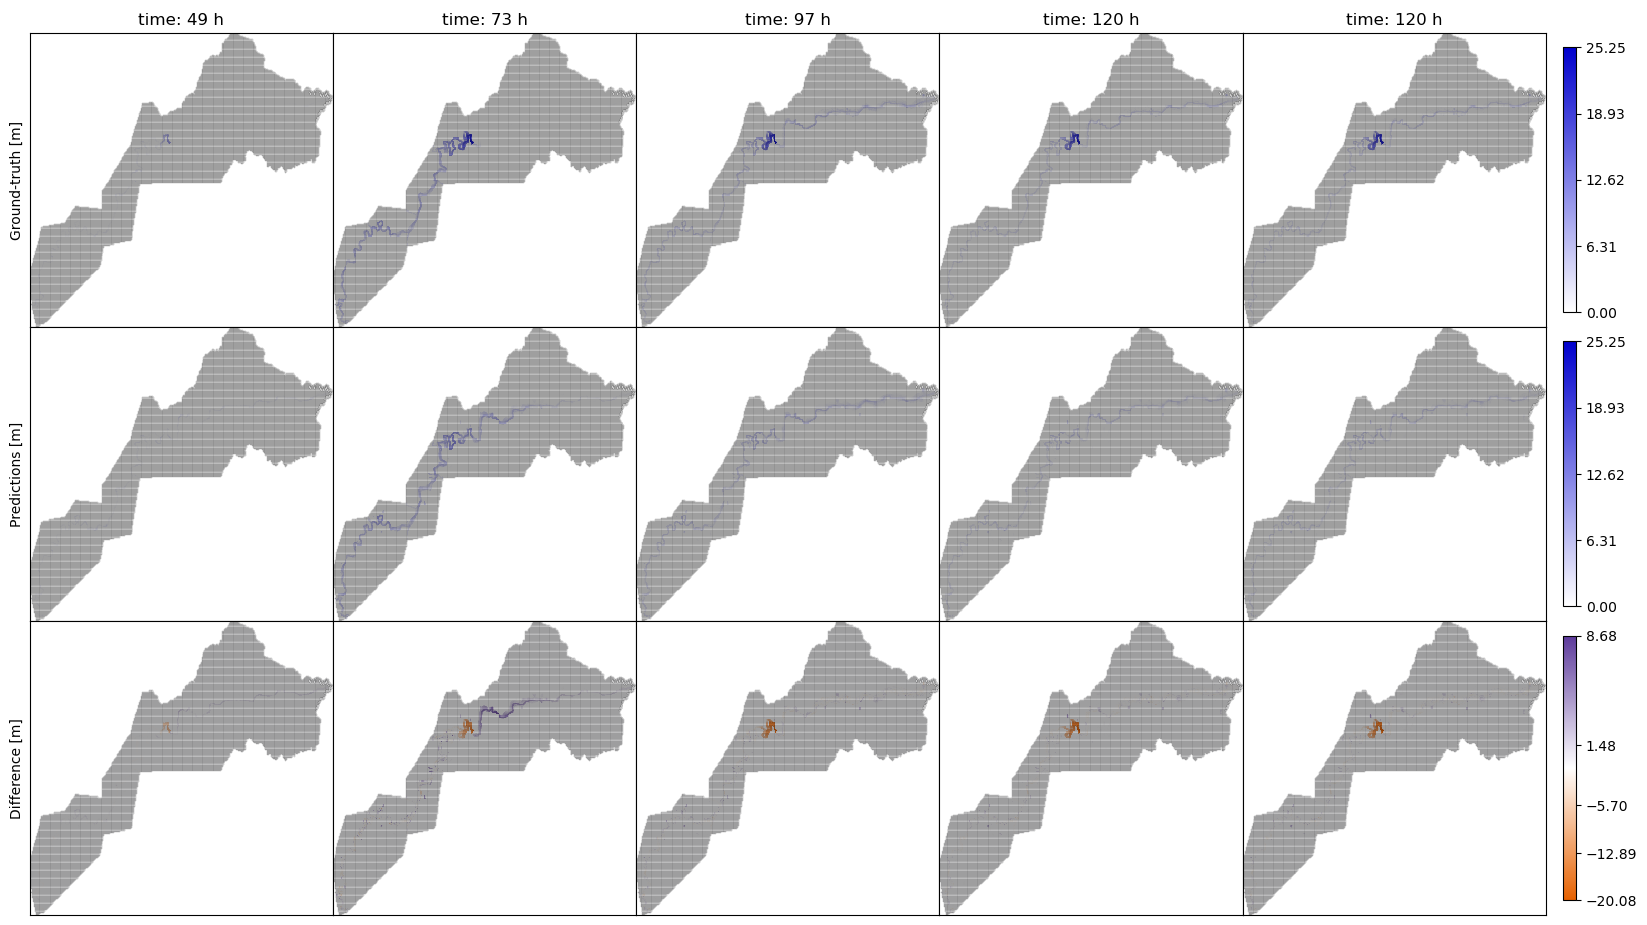
\includegraphics[width=1\textwidth]{failed_thin_dam_20m.png}
  \caption{Structure-aware model on the trained flow obstruction crossing at crest $+15$~m,
    one of the twelve scenarios actually used for training.
    SFINCS ground truth vs.\ prediction at four rollout timesteps.}
  \label{fig:thindam-training-fail}
\end{figure}
 
A concrete explanation follows from how few mesh edges each structure type
actually reaches. Counting edges with a nonzero \texttt{edge\_weir\_crest} value on
the finest mesh scale: the trained thin-dam
crossing tags only 36 of 113{,}230 edges (0.03\%), against 294--324 edges (0.26--0.29\%)
for the levee scenarios. Since this feature is
zero almost everywhere in the graph by construction (Section~\ref{subsubsec:structures_gnn}), the model has to learn its hydraulic effect from a very small,
localised set of training examples, giving the network a small signal to learn from. 
Combined with the small number of flow obstructions scenarios in the twelve-event training set plausibly explains the causes of the model's struggle.
 
 
\subsection{Physical-Consistency Checks}
\label{subsec:res_structures_sensitivity}
 
The remaining diagnostics of Section~\ref{sec:physics_sensitivity_method}, the
magnitude-scaling test, its extrapolation to 2$\times$/3$\times$, and the
catchment-emptying check, all use forcing drawn from the same simulations shared with
the twenty-simulation model's own training set (Section~\ref{sec:res_twenty_sim}).
The structure-aware model behaves the same way as the twenty-simulation model on
every one of them, which is the expected outcome.
 
%\subsection{Summary}
%\label{subsec:res_structures_summary}
 
%The crest-height edge encoding produces a large, measurable hydraulic effect
%(Section~\ref{subsec:res_structures_sanity}) and generalises well for the levee
%scenarios tested, at a modest cost to core-event accuracy
%(Section~\ref{subsec:res_structures_core_accuracy}). It generalises far less well for
%the thin-dam scenarios, and the in-training-set check shows this is a genuine
%representation difficulty rather than a held-out generalisation gap
%(Section~\ref{subsec:res_structures_asymmetry}). For the levee case, the results
%support using this model for what-if scenario analysis without SFINCS ground truth
%(SQ5); for the thin-dam case, predictions on new configurations should be treated with
%more caution, and the physical-plausibility diagnostics of
%Section~\ref{sec:physics_sensitivity_method} (Section~\ref{subsec:res_structures_sensitivity}) are the closest available check in the absence of a
%reference simulation.
 
 
\chapter{Conclusions and Future Work}
\label{ch:conclusions}
 
\section{Answers to the Research Questions}
\label{sec:conclusions_rqs}
 
Extending mSWE-GNN from a single dike-breach point source to fluvial forcing (SQ1)
required two changes beyond a new boundary-condition mechanism, though the
ghost-cell interface itself generalised cleanly from one inflow point to seven.
Transfer learning could not bridge the domain gap: zero-shot inference with the
pre-trained dike-breach weights failed outright (CSI~$=0.000$), and fine-tuning did
not outperform training from scratch. And training from a dry initial condition
failed entirely, the message-passing gradient term that suppresses backflow from
dry cells leaves the network nothing to propagate from, collapsing training to a
near-all-dry prediction regardless of hyperparameters. Loss and mesh-scale choices
refined performance further but were secondary to these two.
 
Hydraulic interventions (SQ2) are represented as a single additional edge feature, crest height, at the finest mesh scale only. Adding a structure also changes the mesh triangulation itself, since the structure polyline is embedded as a constrained edge, so a structure scenario differs from a plain one in mesh geometry as well as in this extra feature. Because the twenty-simulation model was trained on neither, it collapsed domain-wide when tested on a structure scenario, a failure attributable to the unfamiliar mesh. Once retrained, the representation
generalised quite well for levee scenarios but not for flow obstruction ones, and the thin-dam
failure held even on structure configurations included in training, ruling out generalisation as the cause. The likely
explanation is representational scarcity: the flow obstruction crossing tags only 36 of
113{,}230 mesh edges, an order of magnitude fewer than the levee scenarios.
 
On accuracy (SQ3), the best configuration, twenty simulations, reached
CSI@0.05~$=0.853$ and CSI@0.30~$=0.899$ on an event held out entirely from
training. On speed, the literature's headline figures do not transfer: against
SFINCS, the GNN is not faster on CPU ($0.4\times$) and only modestly faster on GPU
($1.4\times$). This reflects the baseline, not the adaptation: SFINCS is already an
accelerated, subgrid-corrected solver, leaving far less headroom than the
full-resolution solver the dike-breach literature compared against.
 
Performance on the Ahr catchment (SQ4) scales with training diversity. A
single-simulation model's response is on/off, not scaled to magnitude; four
simulations fix this; twenty simulations improve further, most clearly in
attributing response to individual source locations by volume share. One
limitation persists regardless of training-set size: complete catchment drainage
was never learnt, plausibly because only one of twenty training simulations
demonstrates it. Which reconstruction method built the ungauged-tributary forcing,
by contrast, made little difference, RMSE spread comparable to ordinary
seed-to-seed noise.
 
Whether the surrogate can be trusted for what-if analysis without a SFINCS
reference (SQ5) comes down to the same three questions in every case examined
here, not a single global answer. Has the model seen this \emph{kind} of scenario
before, even approximately? The single-simulation model never saw varying
magnitude and could not respond to it. How far does the test scenario sit from the
training range in \emph{magnitude}? The held-out levee at twice the highest
trained crest height narrowed the flood correctly but not as tightly as SFINCS,
the same graceful degradation seen in the four-simulation model's extrapolation
tests. How densely was that configuration \emph{represented} in training,
regardless of whether it was formally included? Both the catchment-emptying
scenario and the flow obstruction structure were in the training set, yet both failed,
because each was backed by only a handful of examples. Scenario type, distance in
magnitude, and density of representation are
what separate a trustworthy prediction from an untrustworthy one.
 
Taken together, mSWE-GNN can be adapted to fluvial flooding, but not as a drop-in
extension, and reaches good accuracy once trained on a sufficiently diverse set of
scenarios. What does not hold up is the assumption, inherited from the dike-breach
literature, that this accuracy comes bundled with a large speed advantage: against
SFINCS, that advantage is marginal at best and negative on CPU. The adaptation is
therefore a genuine contribution for accuracy and scenario-based analysis, but its
case for computational efficiency depends on what it is compared against.
 
 
 
\section{Limitations and Recommendations}
\label{sec:limitations_future_work}
 
Several limitations stem from the scope and constraints of the project itself.
 
Nearly every finding in this thesis rests on a single real event: the July 2021 Ahr flood, reconstructed as scaled, perturbed, or structurally augmented variants of it, not on independent storms with genuinely different spatial rainfall patterns or return periods. The twenty- and thirty-two-simulation training sets, while an improvement over a single simulation, are still small in absolute terms; the clear accuracy gains from four to twenty simulations suggest more data would help further, particularly for some specific behaviours like complete catchment drainage and structure representation, that remained undertrained throughout. Transfer-learning conclusions (zero-shot, fine-tuning, cold-start) likewise rest on a single pre-trained source model (DK15); whether they hold for a differently-trained source is untested. The model was trained and evaluated on the Ahr catchment alone, so generalisation to an unseen basin was not assessed here.
 
A second limitation concerns what the reported accuracy is actually measured against. The GNN's RMSE and CSI figures throughout this thesis are computed relative to SFINCS output, not directly against reality; SFINCS's own fidelity to gauge and flood-extent observations is imperfect and only partly explained (Section~\ref{sec:res_sfincs_validation}), and the fixed-zero-depth outflow boundary condition introduces an artefact in the downstream-most reach. The surrogate's accuracy is therefore bounded by the reference simulator's own accuracy, not by the real event directly.
 
Finally, the physical-consistency checks and the comparison across ungauged-tributary reconstruction methods were both conducted using synthetic perturbations of the same event and the same catchment, rather than independent simulations, a real inventory of structure geometries, or gauged confirmation for the ungauged tributaries themselves. This constrains how far the generalisation claims in this thesis can be extended, particularly to a storm of materially different character or return period than July 2021.
 
These limitations point to concrete next steps along the same three lines.
 
For data diversity, training on independent storm events, with genuinely different spatial rainfall patterns, timings, and return periods, would test whether the accuracy gains already seen from one to twenty simulations continue, and whether the specific undertrained behaviours found here, are fixed by targeted additional examples. Applying the same pipeline to a second catchment would test cross-basin generalisation directly, but the mesh-overfitting already found on the structure-augmented mesh (Section~\ref{subsec:res_structures_sanity}) suggests this test would fail for that reason; reducing the model's dependence on one mesh's own statistics is arguably a prerequisite.
 
The fixed-zero-depth outflow boundary and its downstream artefact (Section~\ref{sec:res_sfincs_validation}) are a SFINCS-side limitation that propagates into every GNN result reported here; revisiting that boundary treatment, or excluding the affected reach from evaluation, would remove this confound before further surrogate development.
 
For structures, training on a wider range of scenarios, and other intervention types altogether, would test the representation's reach and address the flow obstruction data-scarcity problem directly. For the ungauged tributaries, estimating discharge with a dedicated rainfall-runoff model would let the reconstruction methods used here be scored against an independent physical model.
 
The false-positive over-wetting identified in Section~\ref{sec:res_fp_overwetting} should be targeted directly in future work, rather than assumed to shrink further as an incidental effect of more training data.

Finally, running the physical-consistency diagnostics against independent simulations, rather than perturbations of one event, would test whether they can catch a genuinely novel failure mode.

\section{Societal Relevance}
\label{sec:societal_relevance}

Beyond the specific gap this thesis addresses, the broader topic carries clear
societal weight. Climate change is already increasing the frequency and severity of
extreme hydrological events \citep{ipcc2021ar6}, and a growing share of society will
have to plan around exactly the kind of riverine flooding studied here. Flood
modelling tools that can be run quickly and repeatedly, across many scenarios, are
directly relevant to that adaptation effort.
 
This thesis contribution is a systematic account of where an
existing, promising framework (mSWE-GNN) works and where it does not, once applied
outside the setting it was originally designed for. That account is itself of
practical value: water authorities and emergency services deciding whether to adopt a
GNN-based surrogate need this kind of evidence.

Fire departments and water boards could use the model to generate flood-extent maps across a range of discharge magnitudes and
return periods, supporting evacuation planning, provided the scenario in question
stays close to the conditions this thesis found the model to handle well. 

On speed in absolute terms, the GNN produces a full multi-day flood forecast in
roughly 27 seconds on CPU and 7 seconds on GPU, comfortably within the response window
needed for an evacuation decision.
 
If a water authority's actual goal is what-if analysis
of structural interventions on a basin, levees, retention areas, or similar, deliberate, careful attention to training-scenario design would be needed. 


% =================================================================
% BIBLIOGRAPHY
% Compiled from every (Author, Year) citation found in the thesis text.
% This document uses plain-text citations rather than \cite{}/BibTeX, so
% entries are given here as a formatted reference list to paste into a
% References/Bibliography chapter, in the same style.
%
% VERIFICATION STATUS:
%   No tag       = verified this session via direct source lookup.
%   [VERIFY]     = compiled from strong prior knowledge (well-established
%                  textbooks/papers) but NOT individually re-checked this
%                  session - low risk, but confirm before submission.
%   [UNVERIFIED] = could not be confirmed with confidence; details below
%                  are best-effort placeholders. DO NOT cite as-is -
%                  locate the actual source before submitting.
% =================================================================
 
\bibliographystyle{apalike}   
\bibliography{references}     

% -----------------------------------------------------------------
% NOT YET CITED WITH A SOURCE IN THE THESIS TEXT -- flagged inline
% where they appear, needs a citation added:
%   - "Delft3D-FM" (Section~\ref{subsec:res_single_sim_accuracy},
%     \textcolor{blue}{note:should cite this} already present in your draft)
%   - "LARSIM" (Section~\ref{subsec:july2021}, mentioned with no citation
%     at all -- likely LARSIM Development Group / Bavarian State Office
%     for the Environment, but not verified here)
% -----------------------------------------------------------------

%================================================================
% APPENDIX
%================================================================

\appendix

\chapter{Baseline Strategy and Cold/Warm-Start Evidence}
\label{app:baseline}

This appendix supplements Section~\ref{sec:zeroshot-finetune-coldwarm} with the
rollout-level evidence behind the baseline-strategy comparison of
Table~\ref{tab:baseline-strategies}: the pre-trained-weight transfer attempts and
the cold-start failure that motivated the warm-start procedure of
Section~\ref{subsec:initial_conditions}.

\section{Cold-Start Failure}
\label{app:coldstart}

Training from scratch with a fully dry initial condition and upstream point-source
forcing converged to a near-all-dry prediction throughout the autoregressive
rollout (RMSE~$=0.195$~m, CSI@0.05~$=0.054$, CSI@0.30~$=0.024$,
Table~\ref{tab:baseline-strategies}), regardless of training duration or
hyperparameter setup. 

\begin{figure}[H]
  \centering
  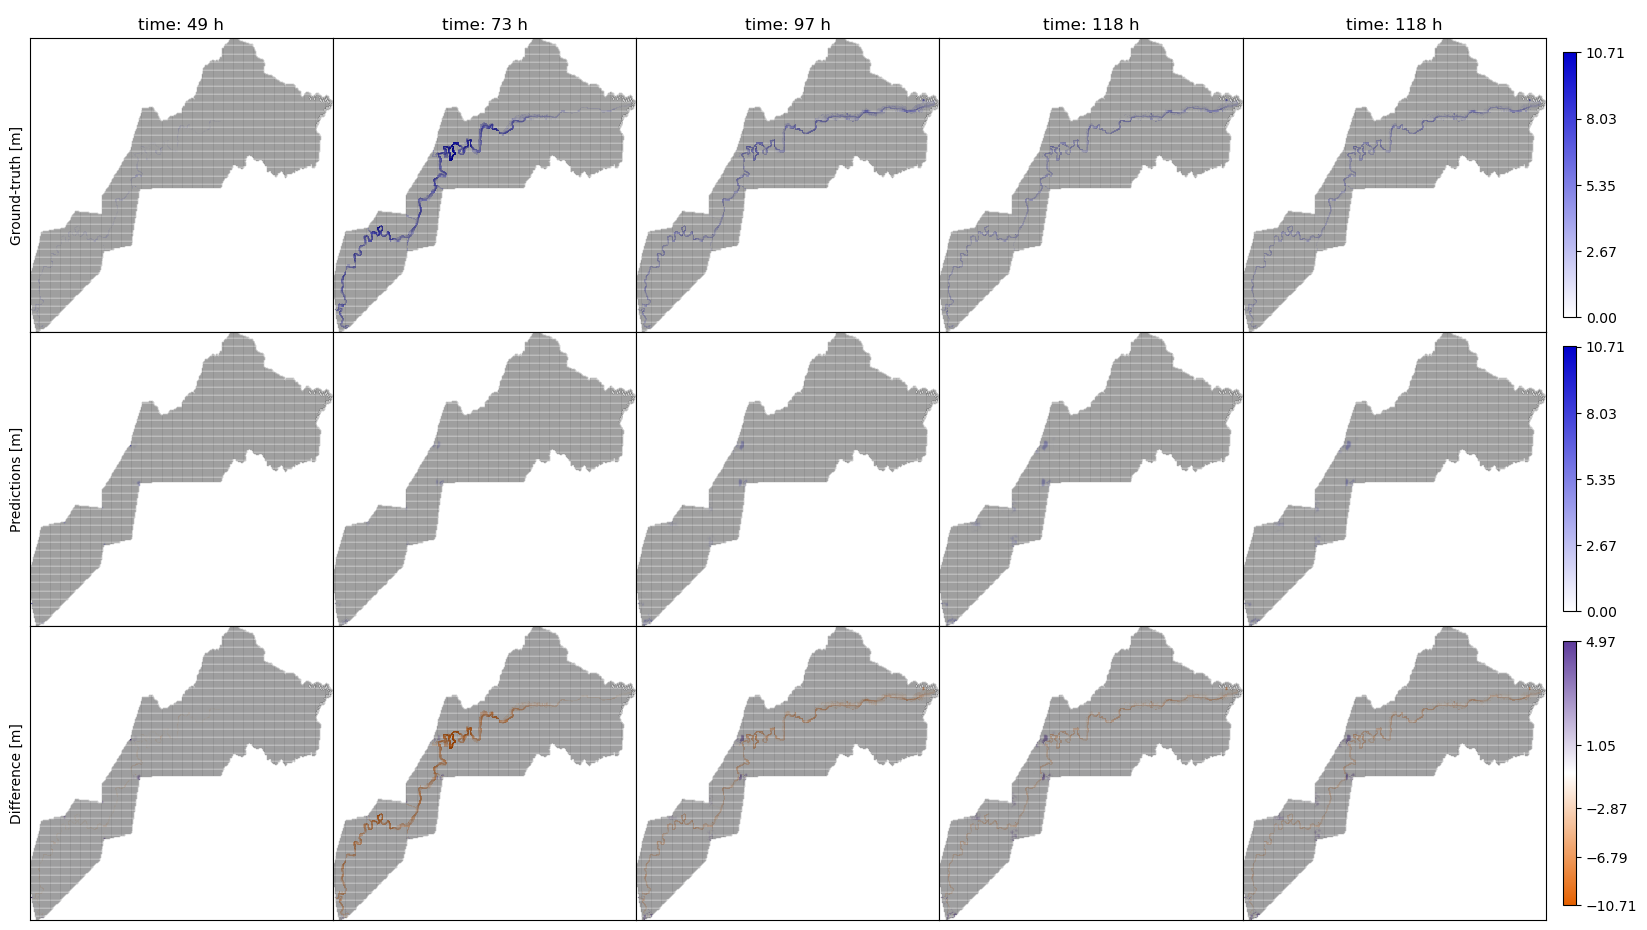
\includegraphics[width=1\textwidth]{coldstart.png}
  \caption{Full-rollout prediction-vs-ground-truth for the cold-start run.}
  \label{fig:coldstart}
\end{figure}

\section{Zero-Shot Transfer from the Pre-Trained DK15 Weights}
\label{app:zeroshot_rollout}

Direct forward inference with the pre-trained mSWE-GNN weights (DK15, Bentivoglio
et al., 2025), without any retraining on Ahr data, produced no meaningful
inundation anywhere in the domain.

\begin{figure}[H]
  \centering
  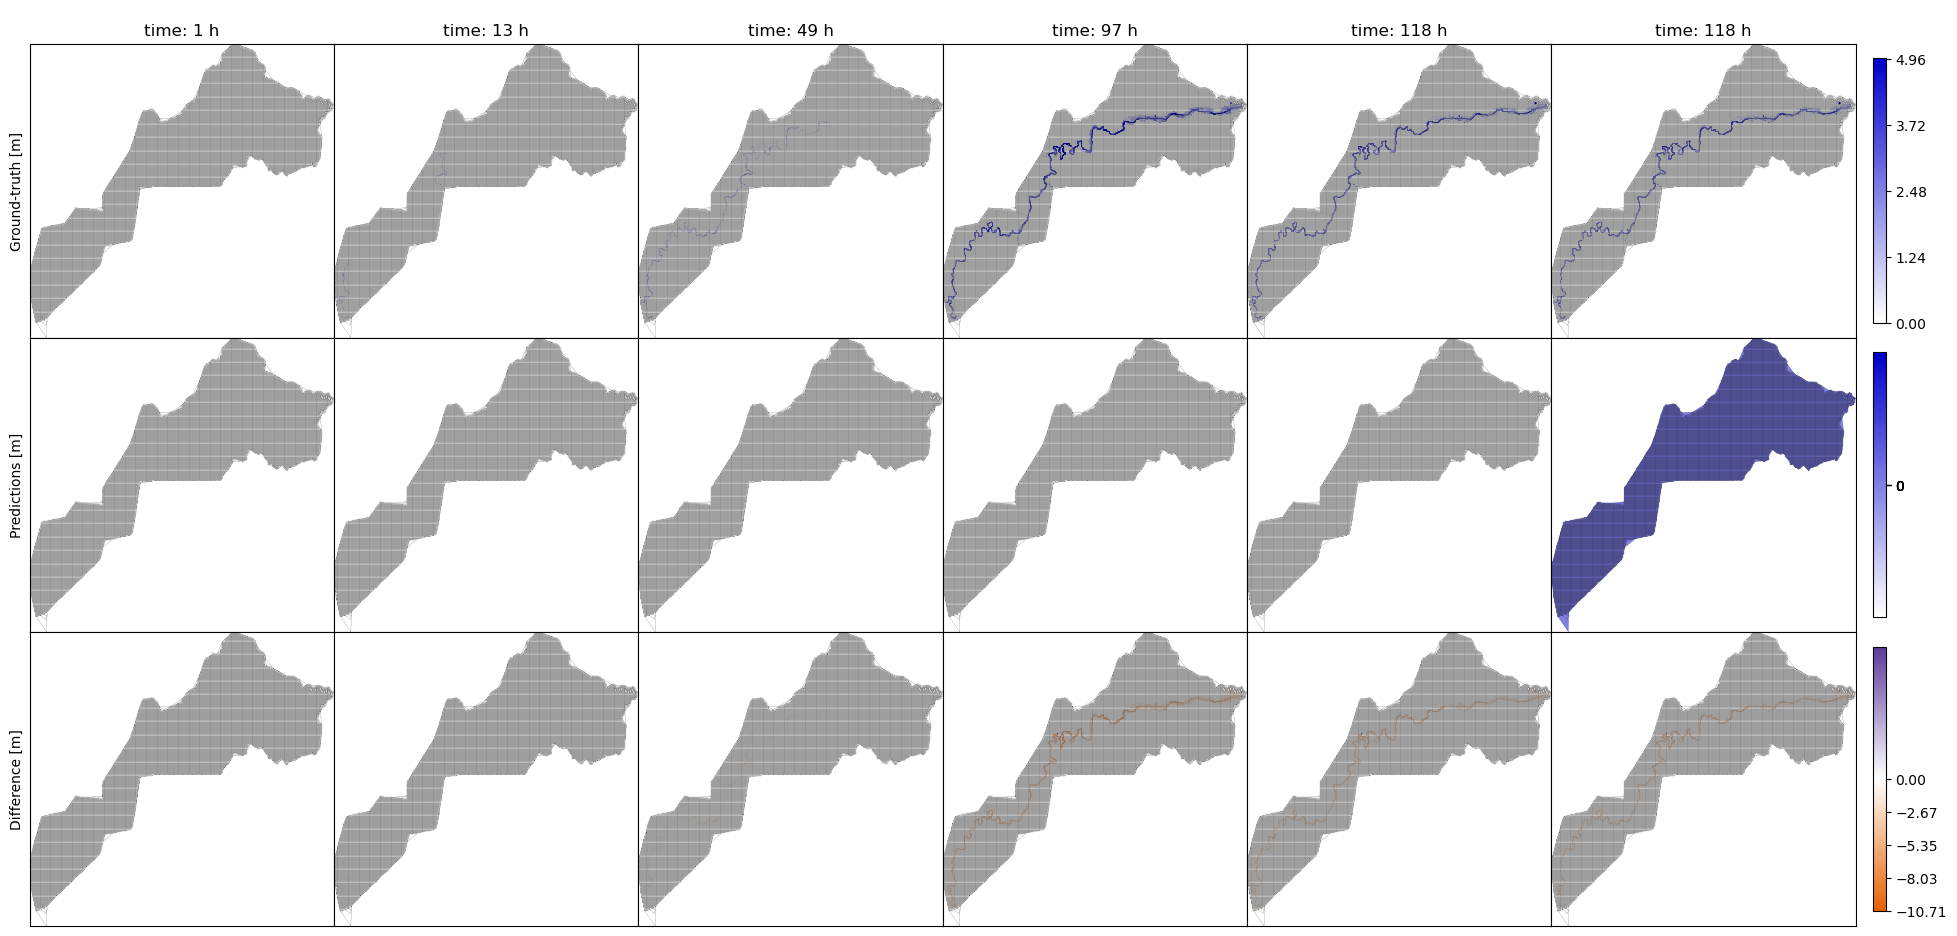
\includegraphics[width=1\textwidth]{interenxe_dk15.png}
  \caption{Full-rollout prediction-vs-ground-truth figure for the DK15 zero-shot run.}
  \label{fig:inferencedk15}
\end{figure}

\section{Warm-Start Ground-Truth Quality: Spinup Length}
\label{app:warmstart_quality}

An earlier version of the warm-start ground truth used a shorter SFINCS spinup
than the 144-hour spinup ultimately adopted (Section~\ref{subsec:warmstart_ahr}),
leaving the final $\approx$7~km of the downstream reach still dry at $t=0$ rather
than hydraulically active. Retraining under the reference configuration
(Section~\ref{subsec:hyperparam_loss}) on the two versions of the ground truth
gives:

\begin{table}[H]
  \centering
    \caption{Effect of spinup length on warm-start ground truth and model accuracy,
      same reference training configuration.}
    \label{tab:app-warmstart-spinup}
    \resizebox{\textwidth}{!}{%
    \begin{tabular}{lcccc}
        \toprule
        Spinup & Wet cells at $t=0$ & RMSE WD [m] & CSI@0.05 & CSI@0.30 \\
        \midrule
        Short (partially dry downstream reach) & 780  & 0.198 & 0.674 & 0.679 \\
        144-hour (fully wetted river)           & 973  & 0.160 & 0.741 & 0.794 \\
        \bottomrule
  \end{tabular}%
  }
\end{table}

\noindent
This comparison is \emph{confounded}: the model was retrained on the new ground
truth rather than only the ground truth being swapped at evaluation time, so the
improvement above reflects both the data change and any incidental differences in
that training run.

\begin{figure}[H]
  \centering
  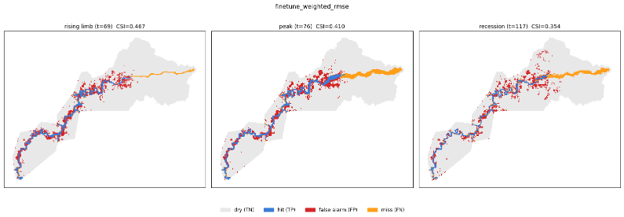
\includegraphics[width=1\textwidth]{before_spinup_fix.png}
  \caption{Spinup run for 48 hr. Model struggling to propagate water in the downstream stretch (same gradient propagation issue encountered with cold start simulation).
}
  \label{fig:b4_fixed_gt}
\end{figure}

\chapter{Training Strategy Development: Design-Choice Trials}
\label{app:training_dev}

This appendix supplements Sections~\ref{subsec:hyperparam_loss} and
\ref{sec:res_hyperparam} with the development history behind the
reference training configuration.

\section{Fine-Tuning from DK15 vs.\ Training from Scratch}
\label{app:finetune_vs_scratch}

\textbf{Question:} does starting from the pre-trained DK15 weights outperform
training from scratch, under otherwise matched conditions?

\textbf{Result:} fine-tuning from DK15 reached RMSE~$=0.191$~m, CSI@0.05~$=0.666$,
CSI@0.30~$=0.778$; training from scratch under matched architecture reached
RMSE~$=0.096$~m, CSI@0.05~$=0.828$, CSI@0.30~$=0.898$
(Table~\ref{tab:baseline-strategies}). Training from scratch outperformed
fine-tuning on every metric.

\textbf{Caveat:} both checkpoints here use hid64 (795k parameters, matched to
each other), not the hid32 reference architecture adopted later; this comparison isolates the transfer-learning
question but not on the final reference architecture.

\textbf{Decision:} training from scratch adopted as the reference strategy for
every subsequent experiment in this thesis.

\section{Mass-Conservation Penalty (Early Comparison)}
\label{app:conservation_early}

\textbf{Question:} does the mass-conservation penalty ($\lambda=0.01$) help or hurt accuracy?

\textbf{Results (historical):} \texttt{rollout5\_hid64\_loss0\_coslr}
is the common baseline for this comparison. \texttt{rollout5\_hid64\_conser=0.01\_loss0\_coslr} adds
the conservation penalty alone on top of that same baseline.
(Figure~\ref{fig:experiments}): the conservation-penalty converges to a plateau comparable to,
the baseline. Qualitatively,
adding the penalty did not visibly improve on the baseline it was added to.

\textbf{Result (clean, single-variable):} re-introducing the penalty
($\lambda=0.01$) alone into the final reference configuration gives
RMSE~$=0.184$~m, CSI@0.05~$=0.614$, CSI@0.30~$=0.763$, below the reference band range.

\textbf{Decision:} penalty removed from the reference configuration.


\section{Shallow-Water-Weighted vs.\ Unweighted RMSE (Early Comparison)}
\label{app:shallow_weight_early}

\textbf{Question:} does up-weighting shallow wet cells ($0 < \mathrm{WD} \le
0.30$~m) in the loss improve accuracy over plain RMSE?

\textbf{Result (historical):} introducing shallow-cell weighting
(initially $w=3$, later swept to $w=5$) improved RMSE from $0.470$~m to $0.262$~m. A weight sweep over $w \in \{3,5\}$
selected $w=5$. (Figure~\ref{fig:experiments})

\textbf{Result (clean, single-variable):} removing the weighting
($w=1$) from the final reference configuration gives RMSE~$=0.155$~m,
CSI@0.05~$=0.660$, CSI@0.30~$=0.804$ (Table~\ref{tab:unweighted-rmse}), below
the reference band range.

\textbf{Decision:} shallow-cell weighting retained, $w=5$, threshold $0.30$~m.

\section{Learning-Rate Schedule: Cosine Decay}
\label{app:coslr}

\textbf{Question:} what learning-rate schedule was used for training, and why?

\textbf{Decision:} a cosine-annealing schedule ($T_\text{max}=1000$, $\eta_\text{min}=1\times10^{-6}$) is used throughout this
thesis. Cosine annealing was adopted early in development, based
on general practice for smooth long-horizon convergence. (Figure~\ref{fig:experiments})

\begin{figure}[H]
  \centering
  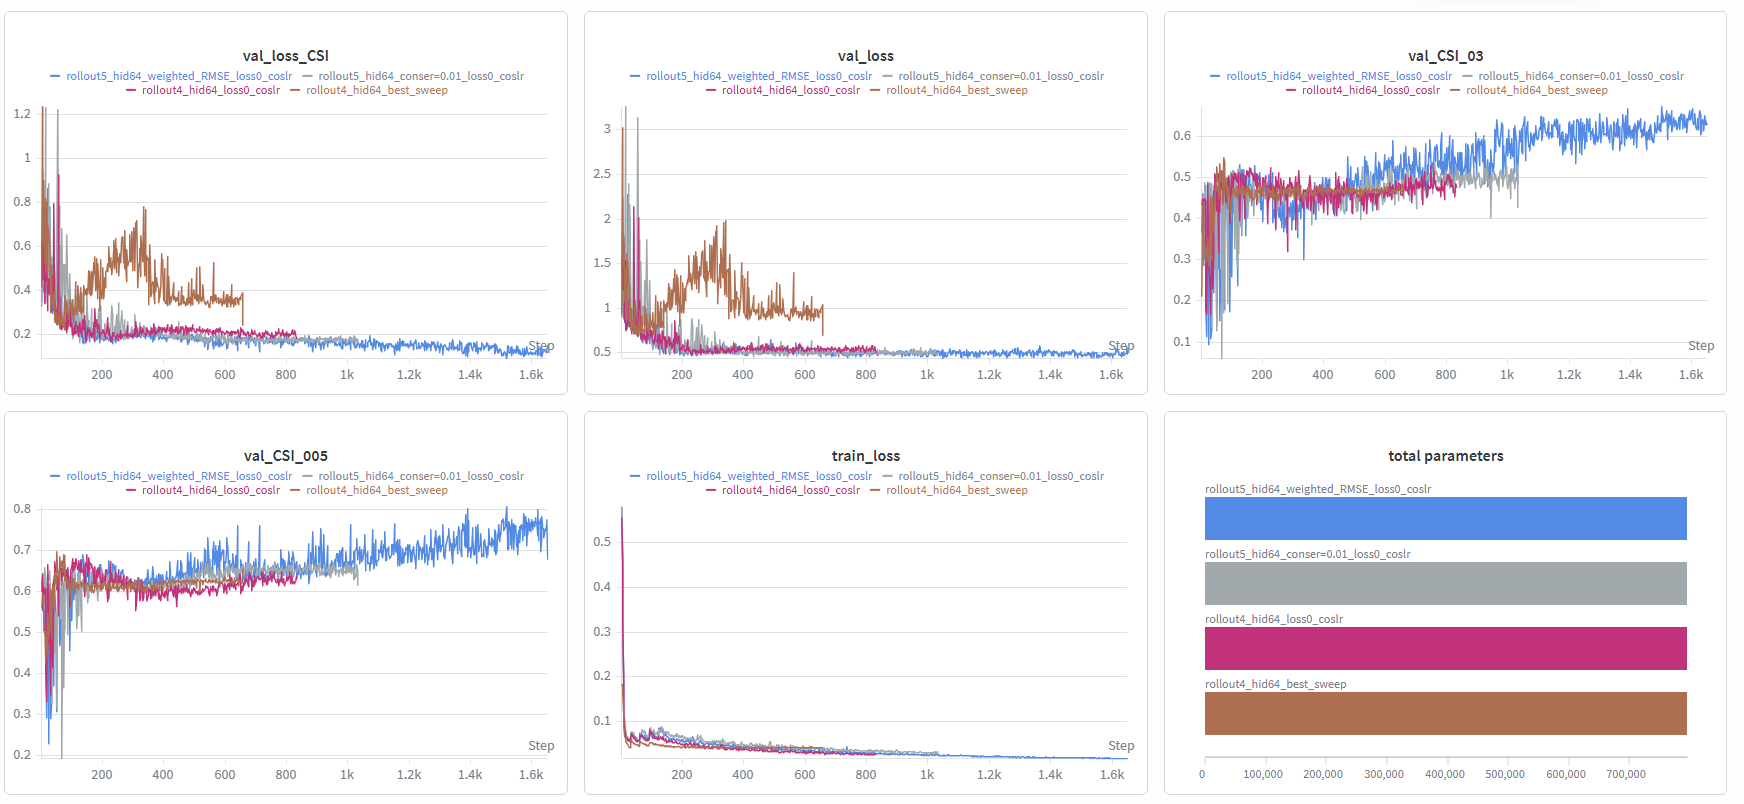
\includegraphics[width=1\textwidth]{experimenting_coslr_weightedrmse.png}
  \caption{Early design choices confrontation (Weights and Biases screenshot).\\
  Blue: Weighted RMSE + cos lr;\\
Gray: Mass conservation coefficient = 0.01 + cos lr;\\
Pink: Varying learning rate (cosine);\\
Brown: Baseline condition.
}
  \label{fig:experiments}
\end{figure}


\begin{figure}[H]
  \centering
  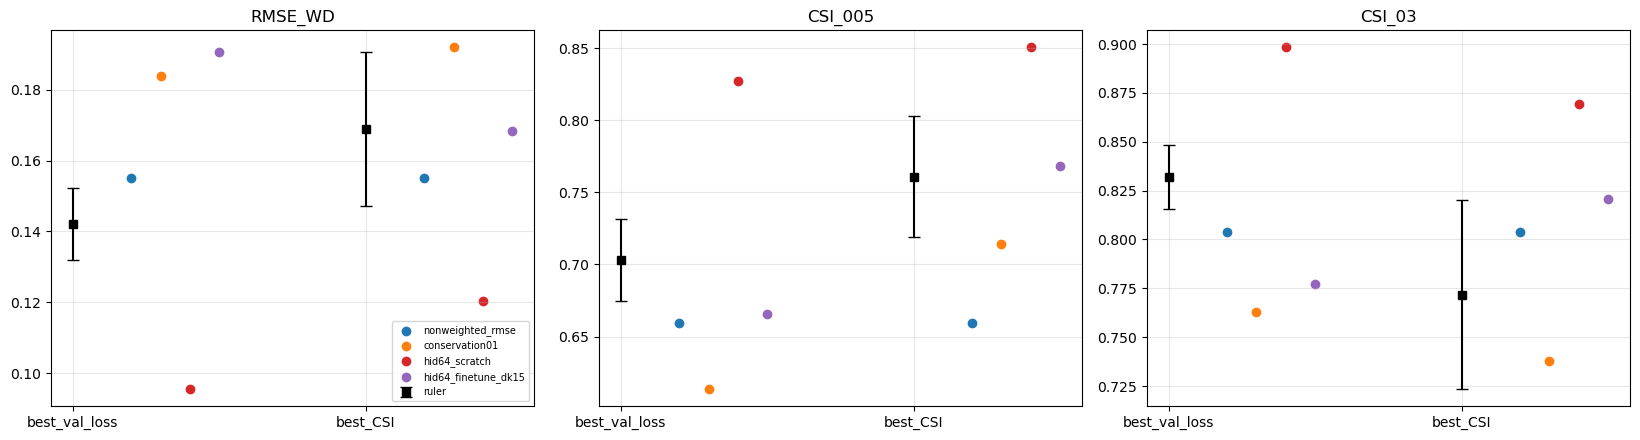
\includegraphics[width=1\textwidth]{ablation_comparison.png}
  \caption{Clean, single-variable ablation (weighted RMS, mass conservation, training vs finetuning)
}
  \label{fig:ablation}
\end{figure}

\section{Loss on All Mesh Scales vs.\ the Finest Scale Only}
\label{app:allscale_loss}

\textbf{Question:} does supervising the loss on all four mesh scales (weights
$[5,1,1,1]$, finest first) improve accuracy over supervising the finest scale
alone?

\textbf{Result:} the all-scale reference configuration reaches
RMSE~$=0.158$~m, CSI@0.05~$=0.775$, CSI@0.30~$=0.832$, above the reference band range. The per-scale
breakdown shows why: under finest-only
loss the coarser scales are effectively unsupervised and their own RMSE degrades
sharply with coarseness (s0~$=0.198$ to s3~$=0.620$), whereas under all-scale
loss the coarser scales stay accurate (s0~$=0.203$ to s3~$=0.213$).

\textbf{Decision:} loss retained across all four mesh scales, with per-scale
weights $[5,1,1,1]$.


\section{Mesh Hierarchy: Four vs.\ Three Mesh Scales (Development History)}
\label{app:mesh_scales_history}

An earlier iteration of this comparison, made with 1 training simulation, showed the same qualitative
result later confirmed by introducing 4 training simulations: removing the coarsest ($\sim$2000~m) mesh level
degraded flood-extent accuracy by introducing a flood front delay.

\begin{figure}[H]
  \centering
  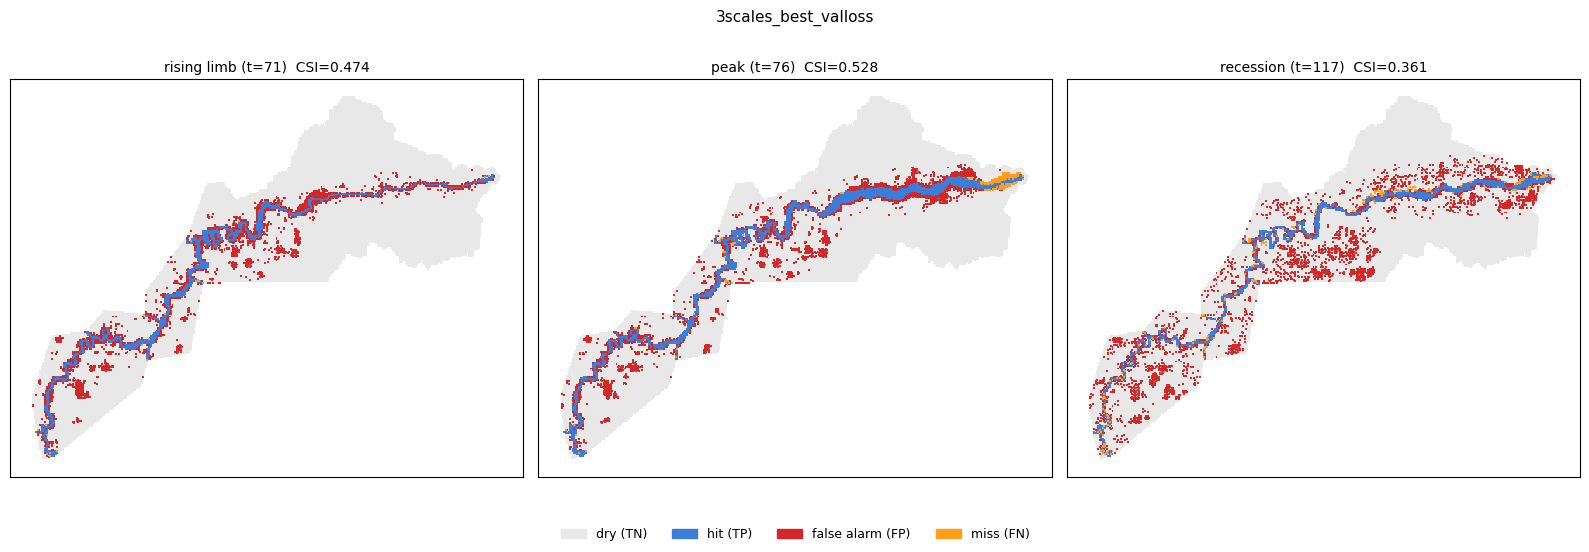
\includegraphics[width=1\textwidth]{3scales_delay.png}
  \caption{Flood front delay, introduced by eliminating the coarser mesh (1 training simulation model)
}
  \label{fig:3scales}
\end{figure}

\begin{figure}[H]
  \centering
  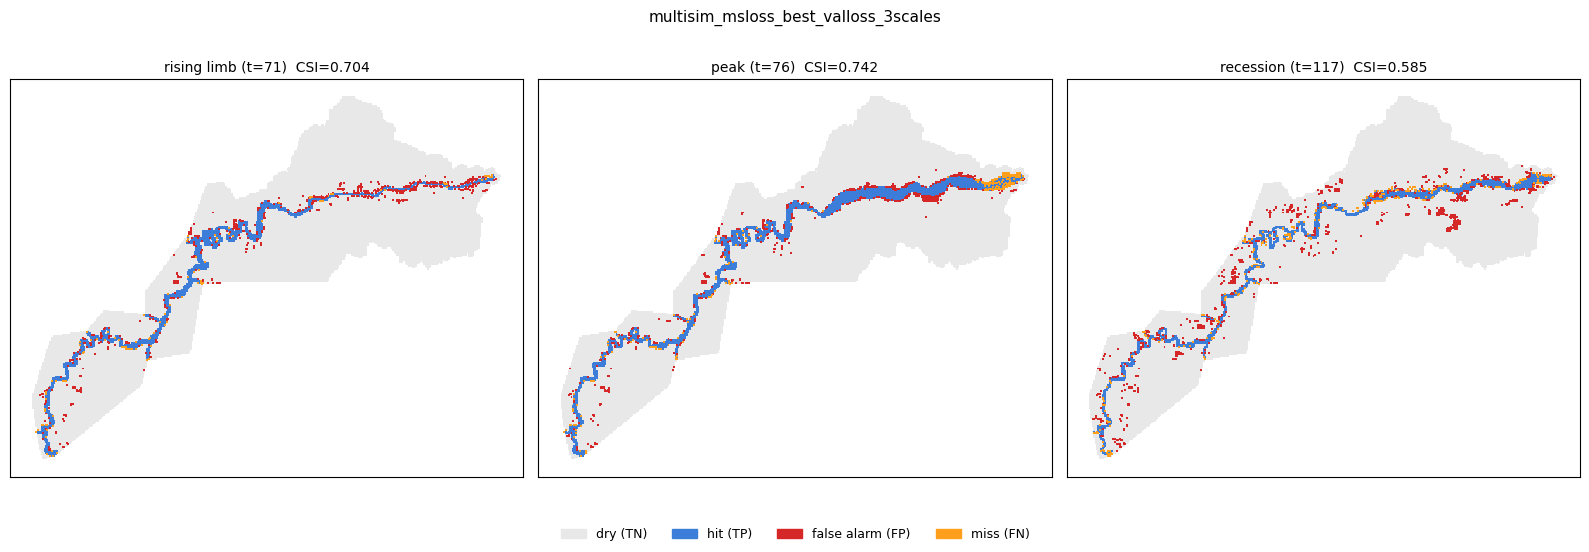
\includegraphics[width=1\textwidth]{3scales_multisim_delay.png}
  \caption{Flood front delay, introduced by eliminating the coarser mesh (4 training simulations model)
}
  \label{fig:3scales_multisim}
\end{figure}

\section{Hyperparameter Sweep}
\label{app:hp_sweep}

\textbf{Question:} does a wider network (hid64, 795k parameters) outperform a
narrower one (hid32, 193k parameters), once hidden size is swept jointly with
the receptive field, learning rate, rollout length, batch size, and shallow-cell
weight, rather than each fixed by hand in isolation?

\textbf{Search grid} (W\&B sweep \texttt{9hskioby}, project
\texttt{mswe-gnn-ahr-sweep}), six dimensions swept jointly:

\begin{table}[H]
    \centering
    \caption{Hyperparameter sweep search space (Bayesian optimization) and the
      winning configuration}
    \label{tab:app-hp-sweep-grid}
    \begin{tabular}{lll}
        \toprule
        Parameter & Values tried & Winner \\
        \midrule
        Receptive field $K$ (per scale) & $[1,1,1,3,3,2,1]$ & \\
                                         & $[1,1,1,5,4,3,2]$ & $[1,1,1,5,4,3,2]$ \\
                                         & $[1,2,2,7,5,4,3]$ & \\
        Learning rate & log-uniform, $[5\times10^{-4}, 3\times10^{-3}]$ & $5.18\times10^{-4}$ \\
        Hidden size  & $\{32, 48, 64\}$ & 32 \\
        Rollout length  & $\{2, 3, 4, 5\}$ & 5 \\
        Batch size & $\{2, 4, 6, 8\}$ & 4 \\
        Shallow-cell weight  & $\{1, 2, 3, 5, 10\}$ & 5 \\
        \bottomrule
    \end{tabular}
\end{table}

\textbf{Result:} the winning configuration is at less than a quarter of
hid64's parameter count.

\textbf{Decision:} hid32 adopted as the reference architecture width; the sweep
configuration frozen as the reference configuration used throughout this thesis.

\chapter{Contents of a Simulation Data Object}
\label{app:sim_data}

This appendix supplements Section~\ref{subsec:sfincs_to_graph} by listing everything
stored for a single simulation once it has been converted from SFINCS output into the
representation used by mSWE-GNN: the dynamic hydraulic fields, the static mesh geometry
and connectivity, the boundary condition data, and the multi-scale structure that ties
them together across mesh resolutions. $N$ is the total number of mesh nodes (faces)
across all $K$ mesh scales,$E$ the total number of edges connecting cells that
share a mesh face, $T$ the number of simulation timesteps, and
$N_{BC}$ the number of boundary condition locations.

\begin{table}[H]
    \centering
    \caption{Quantities stored for a single simulation, once converted into the
      mSWE-GNN representation.}
    \label{tab:app-sim-data}
    \small
    \renewcommand{\arraystretch}{0.9}
    \begin{tabular}{p{4cm}p{2.3cm}p{7.2cm}}
        \toprule
        \textbf{Quantity} & \textbf{Shape} & \textbf{Description} \\
        \midrule
        \multicolumn{3}{l}{\emph{Dynamic hydraulic fields}} \\
        Water depth & $(N,\ T)$ & Water depth time series (Eq.~\ref{eq:waterdepth}) [m] \\
        Velocity components & $(N,\ T)$ & Two arrays, one per horizontal direction [m/s] \\
        \midrule
        \multicolumn{3}{l}{\emph{Static node (face) features}} \\
        Bed elevation & $(N,)$ & Terrain elevation at each mesh node [m] \\
        Cell area & $(N,)$ & Area of the mesh face represented by each node [m$^2$] \\
        \midrule
        \multicolumn{3}{l}{\emph{Static edge features (face-adjacency graph)}} \\
        Edge index & $(2,\ E)$ & Pair of node indices connected by each edge \\
        Face-to-face distance & $(E,)$ & Distance between the centroids of the two faces sharing an edge [m] \\
        Relative face position & $(E,\ 2)$ & Horizontal offset between the centroids of the two faces sharing an edge [m] \\
        Bed slope & $(E,)$ & Bed elevation difference between the two faces sharing an edge, normalised by face-to-face distance [m/m] \\
        Structure crest offset & $(E,)$ & Height of a hydraulic structure's crest above the local terrain, for edges crossed by a structure (Section~\ref{subsubsec:structures_gnn}); zero elsewhere. Present only for hydraulic-structure scenarios \\
        \midrule
        \multicolumn{3}{l}{\emph{Boundary conditions}} \\
        Boundary condition tensor & $(N_{BC},\ T,\ 2)$ & Time series of water surface elevation and unit discharge at each boundary location \\
        Boundary condition type & scalar & Flag indicating whether the boundary condition tensor represents a discharge or a water-level forcing \\
        Boundary node indices & $(N_{BC},)$ & Indices of the ghost-cell nodes at which the boundary condition tensor is applied \\
        Outflow boundary node indices & $(N_{BC,\text{out}},)$ & Indices of the outflow ghost-cell nodes (outflow-enabled datasets only; Section~\ref{subsec:model_adaptation_detail}) \\
        Boundary edge lengths & $(N_{BC},)$ & Length of the boundary edge associated with each boundary node [m] \\
        \midrule
        \multicolumn{3}{l}{\emph{Multi-scale mesh structure}} \\
        Number of nodes & scalar & Total node count $N$ across all mesh scales \\
        Multi-scale mesh object & --- & Per-scale face and edge geometry and topology from which the tensors above are derived (Section~\ref{subsec:multiscale_mesh}) \\
        Scale pointers & $(K+1,)$ & Index ranges delimiting each mesh scale's nodes (and, separately, its edges) within the flattened arrays above \\
        Inter-scale pooling edges & $(2,\ E_\text{pool})$ & Connectivity linking nodes across adjacent mesh scales, together with the pointer delimiting each scale transition \\
        \bottomrule
    \end{tabular}
\end{table}


\chapter{SFINCS Numerical Scheme Parameters}
\label{app:sfincs_params}

This appendix lists the SFINCS-Ahr numerical scheme parameters referenced in
Section~\ref{subsec:model_params}.

\begin{table}[H]
    \centering
    \caption{SFINCS-Ahr numerical scheme parameters.}
    \label{tab:app-sfincs-params}
    \begin{tabular}{llp{6.5cm}}
        \toprule
        Parameter & Value & Controls \\
        \midrule
        Time-step limiter $\alpha$ & 0.5 & Additional restriction on the adaptive time step beyond the CFL condition; lower values improve stability at the cost of speed \citep{leijnse2021sfincs}. \\
        Implicitness factor $\theta$ & 1 & Weighting between the explicit and implicit parts of the momentum-equation solution; lower values add numerical smoothing where the default value is unstable. \\
        Wetting threshold $h_\text{thresh}$ [m] & 0.01 & Minimum water depth for a cell to be treated as wet and included in flux computations. \\
        Advection & on & Whether the advection term is retained in the momentum equation (subcritical shallow water equations) or dropped (local inertial approximation). \\
        Coriolis & on & Whether the Coriolis term is included in the momentum equation. \\
        Viscosity & on & Whether the horizontal eddy viscosity term is included in the momentum equation. \\
        \bottomrule
    \end{tabular}
\end{table}

\chapter{Hydraulic Structure Scenario Design}
\label{app:structure_scenarios}

This appendix lists the sixteen hydraulic-structure scenarios referenced in
Section~\ref{sec:structure_scenarios}: twelve used for training the
structure-aware model and four held out for testing
(Section~\ref{subsec:res_structures_generalisation}).

\begin{table}[H]
    \centering
    \caption{Hydraulic structure scenarios: known parameters. Location A~=~Bad
      Neuenahr-Ahrweiler (levees, parallel to channel margin); Location B~=~Altenahr
      (flow obstructions, perpendicular to flow).}
    \label{tab:structure_scenarios}
    \resizebox{\textwidth}{!}{%
    \begin{tabular}{llcccc}
        \toprule
        Scenario & Location/type & Crest height [m] & Split & Tagged edges & Edges~\% & Notes \\
        \midrule
        flow obstruction, trained location, crest~15~m & B, flow obstruction & 15 & Train & 36 & 0.03\%  \\
        flow obstruction, trained location, crest~20~m & B, flow obstruction & 20 & Train & 38 & 0.03\%  \\
        Levee, both banks, crest~2~m & A, levee & 2 & Train & 264 & 0.23\%  \\
        Levee, both banks, crest~5~m & A, levee & 5 & Train & 298 & 0.26\% \\
        Levee, north bank only, crest~2~m & A, levee & 2 & Train & 142 & 0.13\% \\
        Levee, north bank only, crest~5~m & A, levee & 5 & Train & 158 & 0.14\% \\
        Levee, south bank only, crest~2~m & A, levee & 2 & Train & 122 & 0.11\% \\
        Levee, south bank only, crest~5~m & A, levee & 5 & Train & 154 & 0.14\% \\
        Levee, upstream half, crest~2~m & A, levee & 2 & Train & 134 & 0.12\% \\
        Levee, upstream half, crest~5~m & A, levee & 5 & Train & 162 & 0.14\%\\
        Levee, downstream half, crest~2~m & A, levee & 2 & Train & 128 & 0.11\% \\
        Levee, downstream half, crest~5~m & A, levee & 5 & Train & 148 & 0.13\% \\
        \midrule
        Levee, unseen magnitude, both banks & A, levee & 10 & Test & 324 & 0.29\% \\
        Levee, unseen footprint (breach) & A, levee & 5 & Test & 294 & 0.26\% \\
        flow obstruction, unseen location & B, flow obstruction & 15 & Test & 34 & 0.03\% \\
        flow obstruction, unseen location & B, flow obstruction & 20 & Test & 34 & 0.03\% \\
        \bottomrule
    \end{tabular}%
    }
\end{table}

\begin{figure}[H]
  \centering
  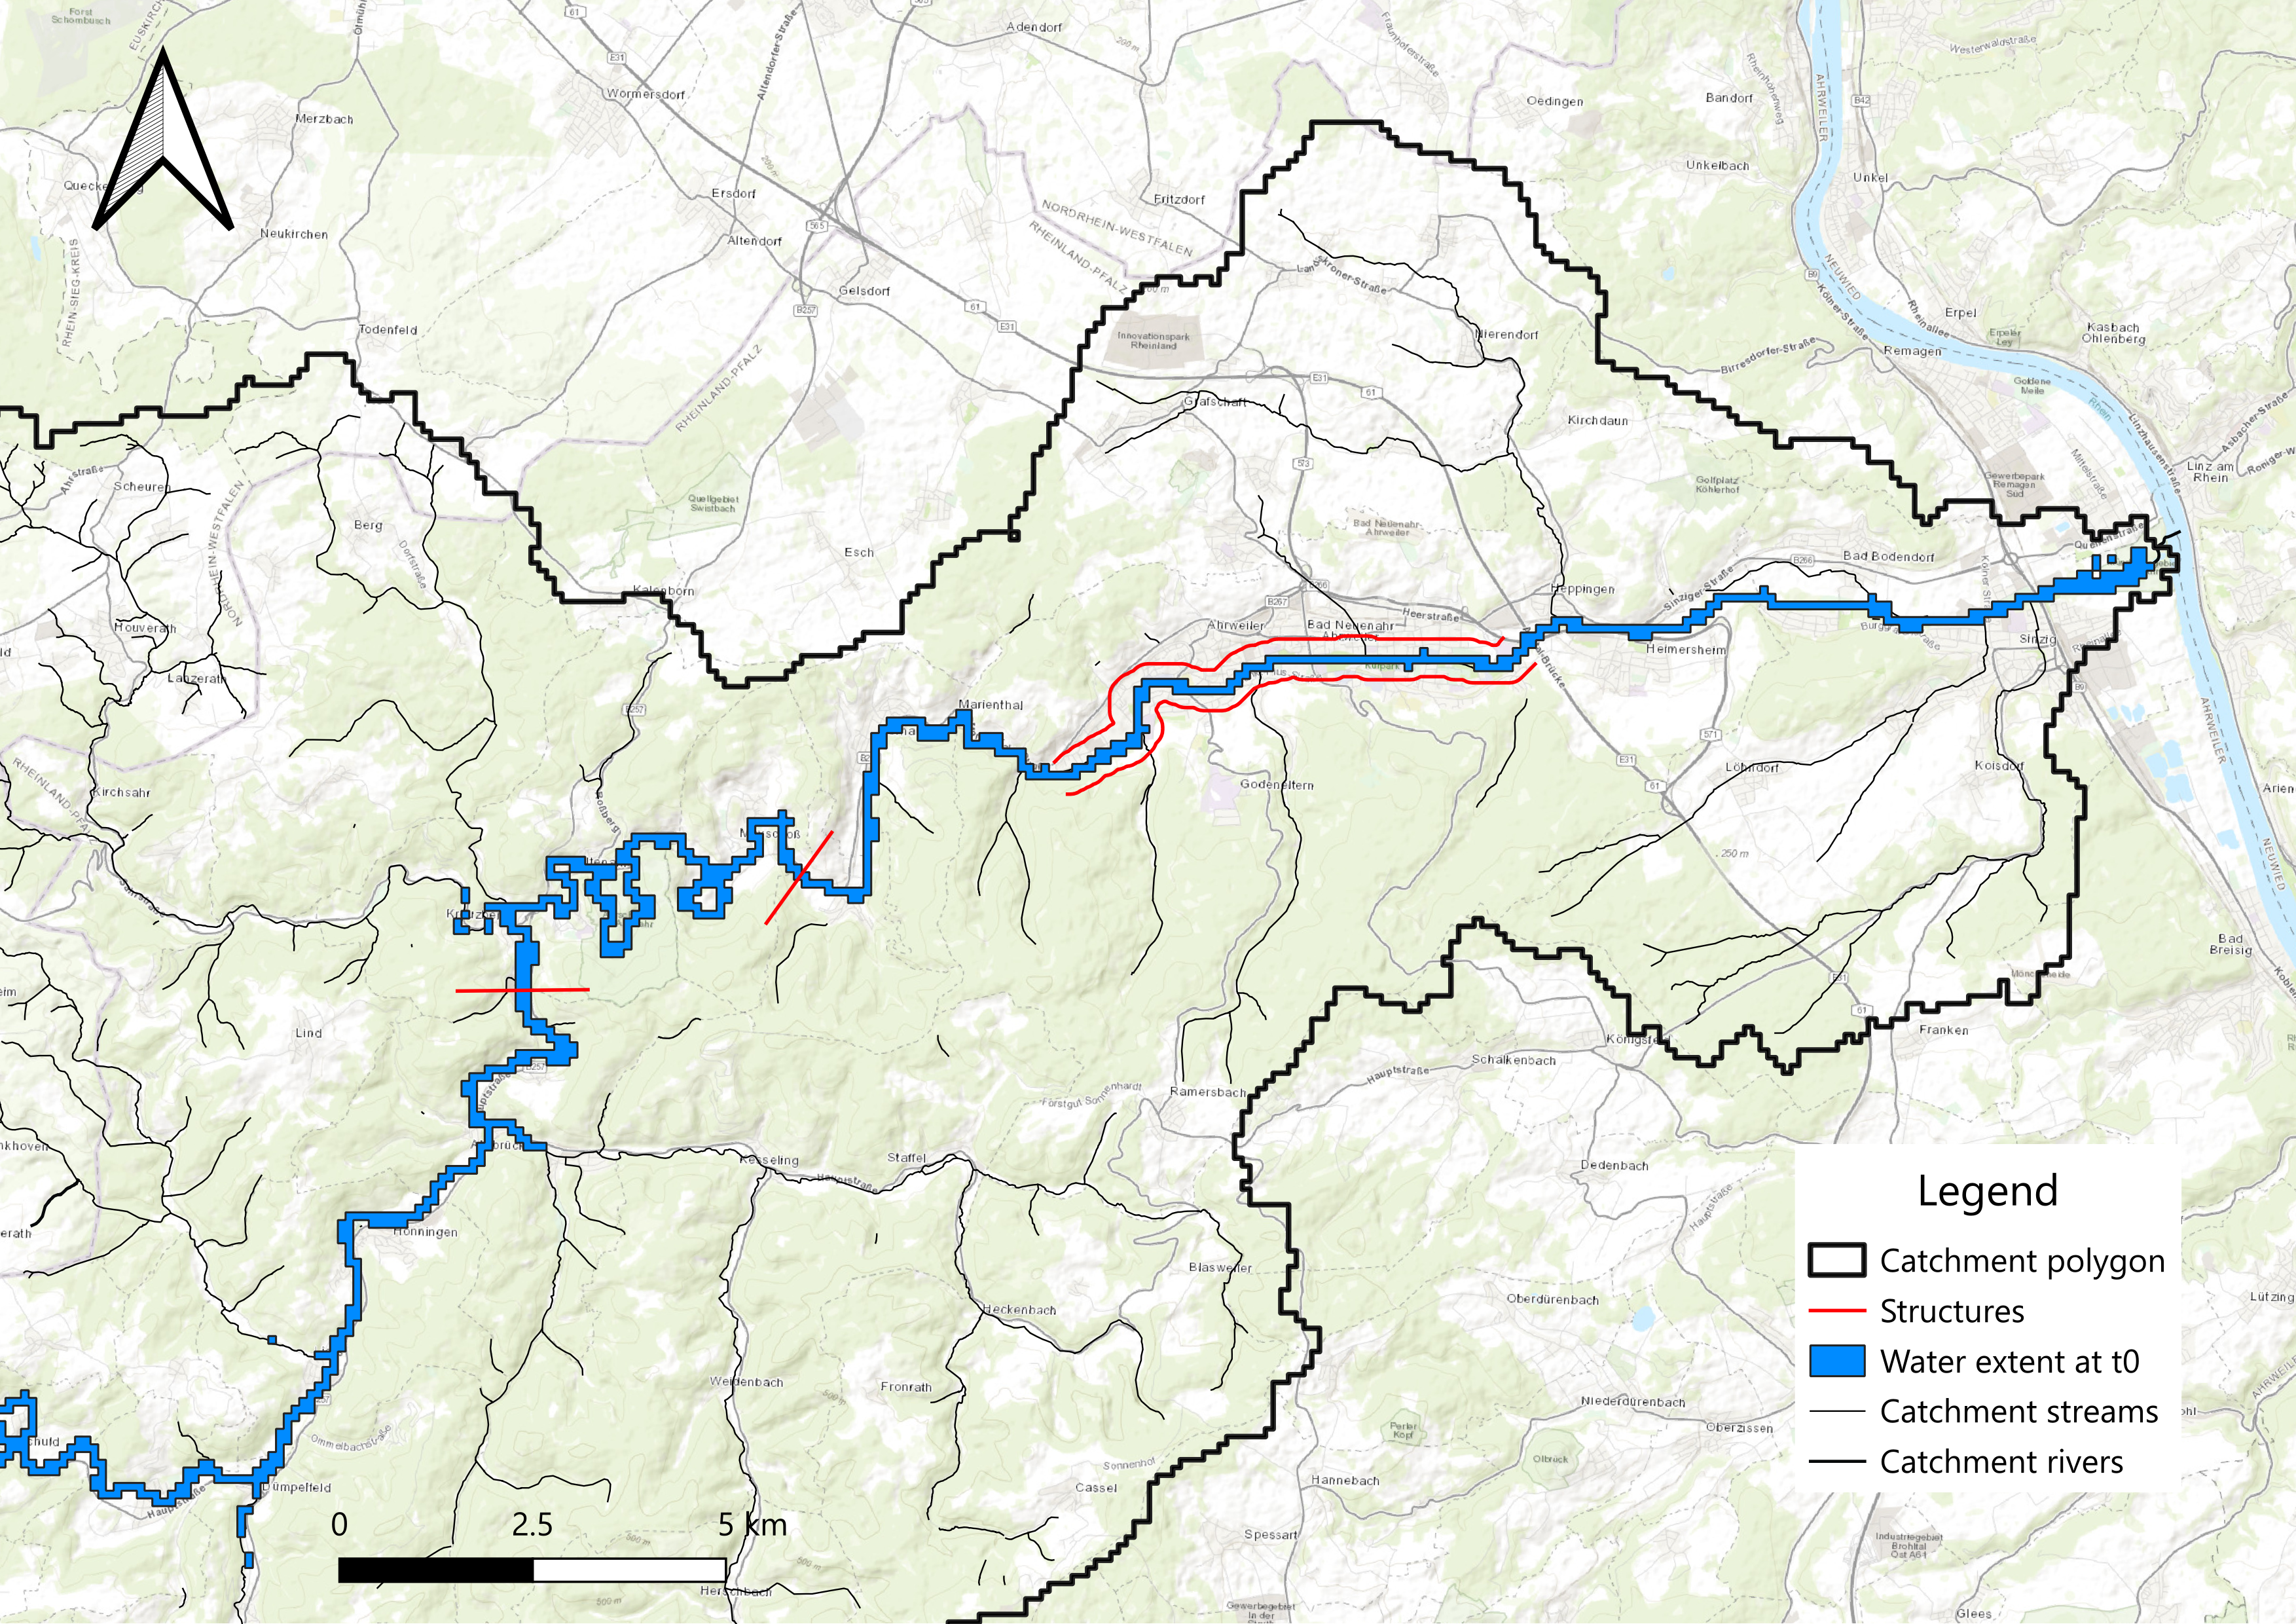
\includegraphics[width=0.8\textwidth]{Structures.png}
  \caption{Structures geometry and location.
}
  \label{fig:structures}
\end{figure}

\chapter{Supplementary Figures: Non-Uniform Forcing Response Maps}
\label{app:nonuniform_maps}

This appendix supplements the leave-one-out and block-BC sensitivity tests of
Sections~\ref{subsec:res_four_sim_sensitivity} and
\ref{subsec:res_twenty_sim_nonuniform} with spatial difference-at-peak maps for
each non-uniform-forcing scenario, referenced from
Section~\ref{subsec:res_four_sim_sensitivity} as evidence for whether a source
perturbation's effect stays spatially confined to the vicinity of that inflow
point or propagates more broadly across the domain.

\section{Four-Simulation Model}
\label{app:nonuniform_maps_foursim}


\begin{figure}[H]
    \centering
    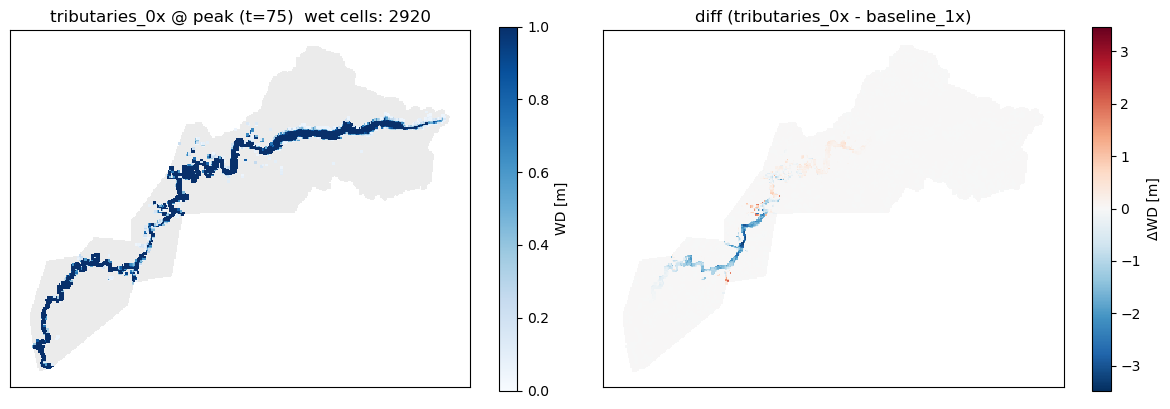
\includegraphics[width=0.8\textwidth]{trib_0X_4_sim.png}
    \caption{Four-simulation model, tributaries scaled to $0\times$ (the three
      smallest tributaries switched off, 18.5\% of forcing volume): real peak
      WD-sum falls 14.4\%, predicted peak falls only 7.2\%
      (RMSE~$=0.144$~m, CSI@0.05~$=0.785$, Table~\ref{tab:foursim-blockbc}).}
    \label{fig:app-e-foursim-trib0x}
\end{figure}

\begin{figure}[H]
    \centering
    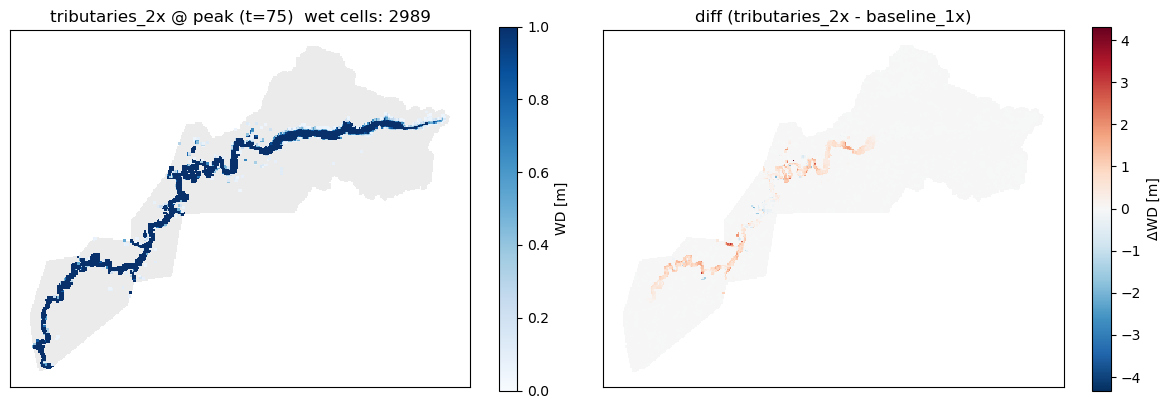
\includegraphics[width=0.8\textwidth]{trib_2X_4sim.png}
    \caption{Four-simulation model, tributaries scaled to $2\times$: real peak
      rises 14.8\%, predicted peak rises 10.8\% (RMSE~$=0.159$~m,
      CSI@0.05~$=0.790$, Table~\ref{tab:foursim-blockbc}).}
    \label{fig:app-e-foursim-trib2x}
\end{figure}

\begin{figure}[H]
    \centering
    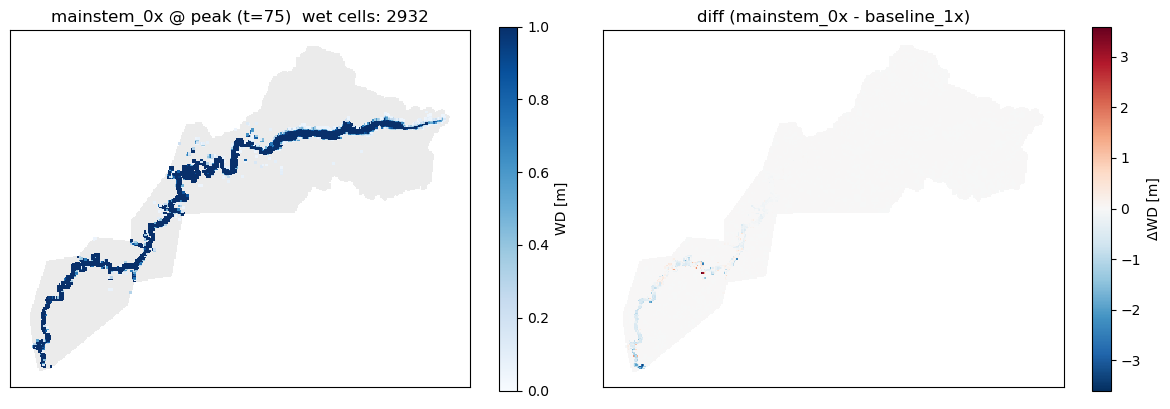
\includegraphics[width=0.8\textwidth]{main_0X_4sim.png}
    \caption{Four-simulation model, main stem (Kirmutscheid, 49.8\% of forcing
      volume) scaled to $0\times$: real peak falls 34.9\%, predicted peak falls
      only 2.9\%, the model's most severely damped magnitude response
      (RMSE~$=0.179$~m, CSI@0.05~$=0.743$, Table~\ref{tab:foursim-blockbc}).}
    \label{fig:app-e-foursim-mainstem0x}
\end{figure}

\begin{figure}[H]
    \centering
    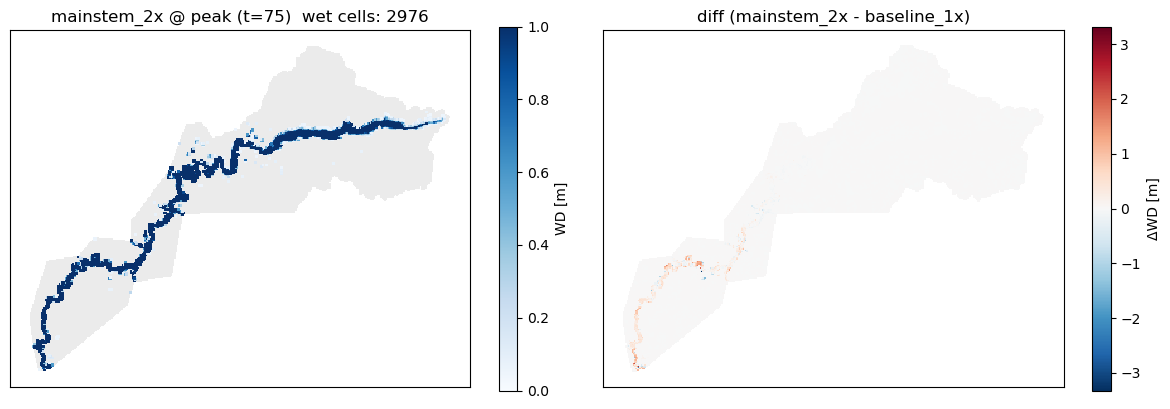
\includegraphics[width=0.8\textwidth]{main_2X_4sim.png}
    \caption{Four-simulation model, main stem scaled to $2\times$: real peak
      rises 28.4\%, predicted peak rises only 2.8\% (RMSE~$=0.205$~m,
      CSI@0.05~$=0.795$, Table~\ref{tab:foursim-blockbc}).}
    \label{fig:app-e-foursim-mainstem2x}
\end{figure}

\begin{figure}[H]
    \centering
    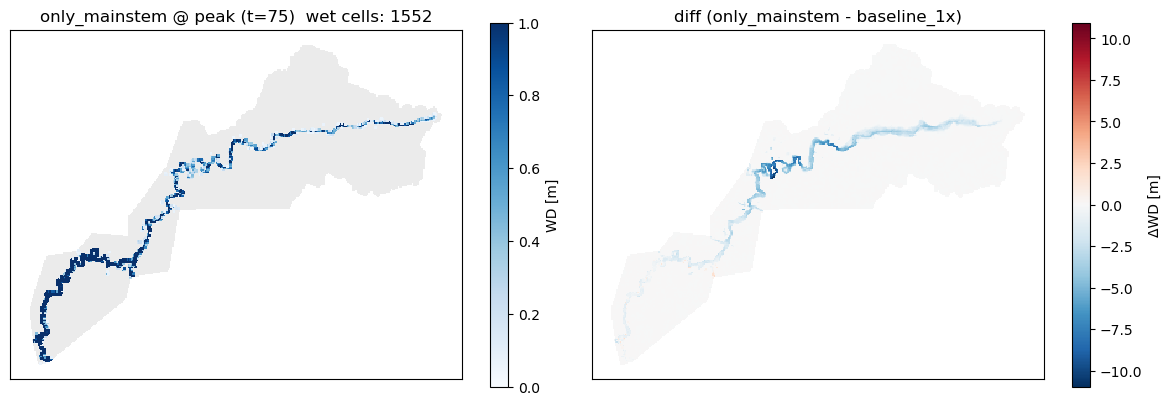
\includegraphics[width=0.8\textwidth]{only_main_4sim.png}
    \caption{Four-simulation model, only the main stem active (all other six
      sources at $0\times$): the model under-predicts badly (real peak 5270,
      predicted 2203) and the predicted peak arrives 10~h too early
      (RMSE~$=0.207$~m, CSI@0.05~$=0.719$, Table~\ref{tab:foursim-blockbc}).}
    \label{fig:app-e-foursim-onlymainstem}
\end{figure}

\begin{figure}[H]
    \centering
    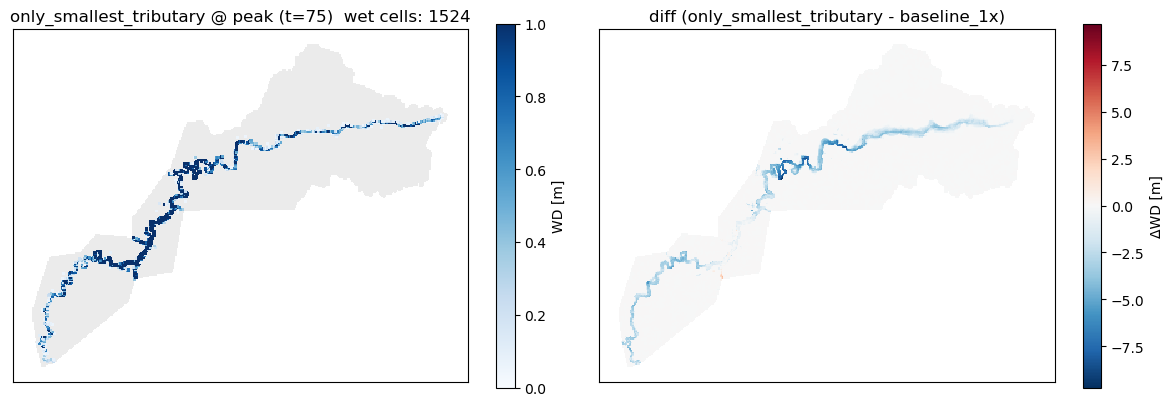
\includegraphics[width=0.8\textwidth]{only_trib_4sim.png}
    \caption{Four-simulation model, only the smallest tributary active (all
      other six sources at $0\times$): the model over-predicts badly (real
      peak 842, essentially no flood, predicted 4898) (RMSE~$=0.205$~m,
      CSI@0.05~$=0.570$, Table~\ref{tab:foursim-blockbc}).}
    \label{fig:app-e-foursim-onlysmallesttrib}
\end{figure}

\section{Twenty-Simulation Model}
\label{app:nonuniform_maps_twentysim}


\begin{figure}[H]
    \centering
    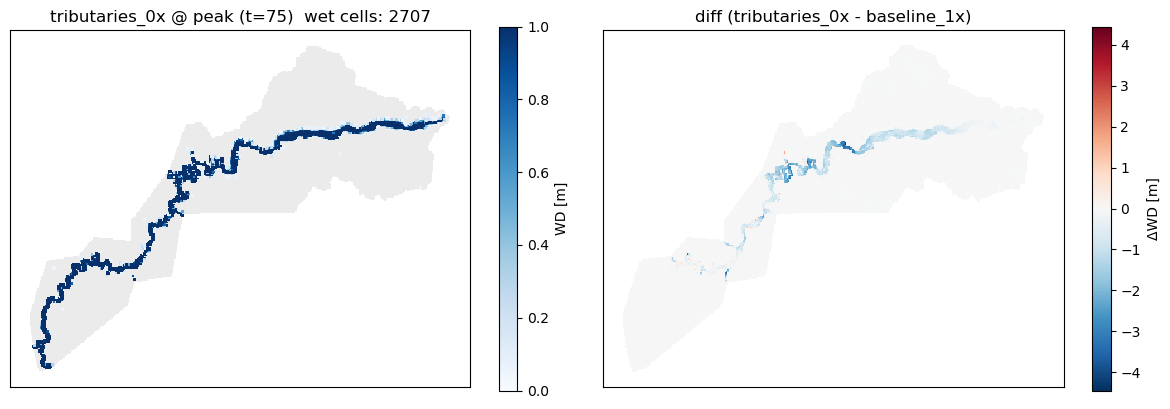
\includegraphics[width=0.8\textwidth]{trib_0X_20sim.png}
    \caption{Twenty-simulation model, tributaries scaled to $0\times$
      (RMSE~$=0.119$~m, CSI@0.05~$=0.833$, Table~\ref{tab:twentysim-blockbc}).}
    \label{fig:app-e-twentysim-trib0x}
\end{figure}

\begin{figure}[H]
    \centering
    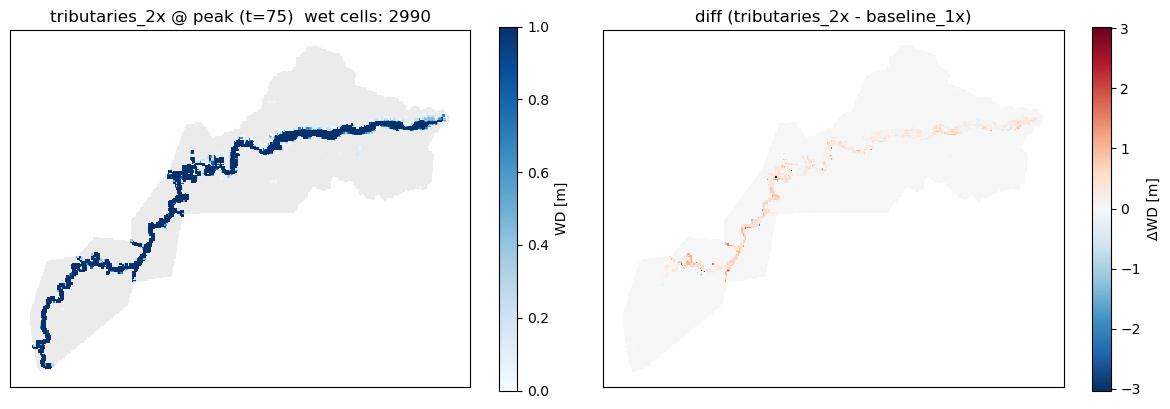
\includegraphics[width=0.8\textwidth]{trib_2X_20sim.png}
    \caption{Twenty-simulation model, tributaries scaled to $2\times$
      (RMSE~$=0.143$~m, CSI@0.05~$=0.829$, Table~\ref{tab:twentysim-blockbc}).}
    \label{fig:app-e-twentysim-trib2x}
\end{figure}

\begin{figure}[H]
    \centering
    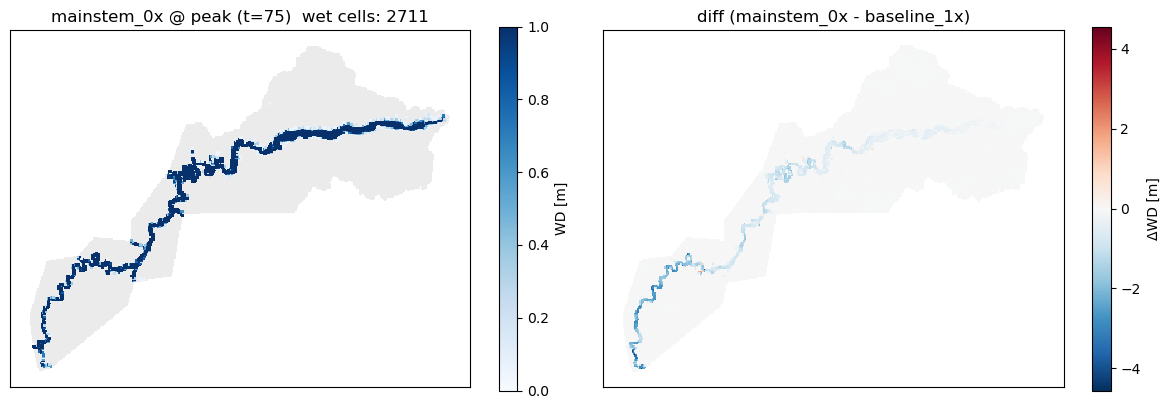
\includegraphics[width=0.8\textwidth]{main_0X_20sim.png}
    \caption{Twenty-simulation model, main stem scaled to $0\times$: peak error
      falls from $+51.9\%$ (four-simulation model) to $+24.6\%$
      (RMSE~$=0.129$~m, CSI@0.05~$=0.810$, Table~\ref{tab:twentysim-blockbc}).}
    \label{fig:app-e-twentysim-mainstem0x}
\end{figure}

\begin{figure}[H]
    \centering
    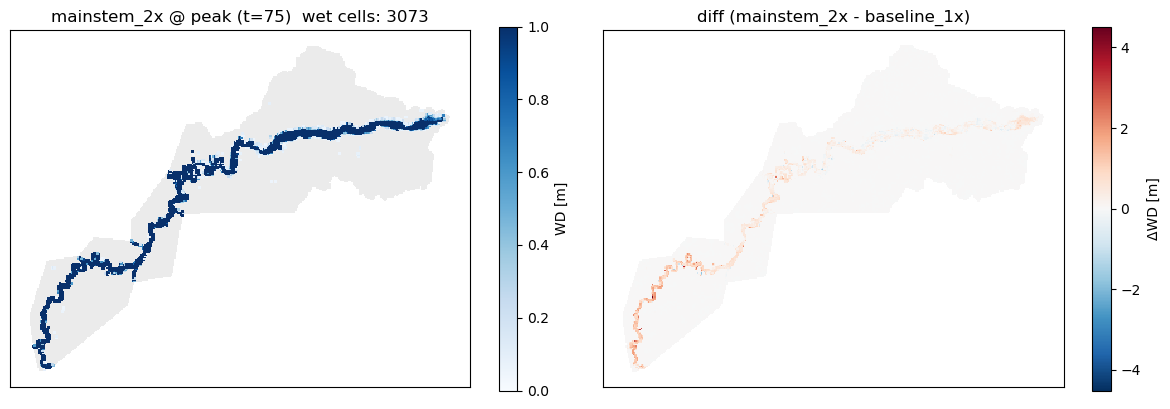
\includegraphics[width=0.8\textwidth]{main_2X_20sim.png}
    \caption{Twenty-simulation model, main stem scaled to $2\times$: peak error
      falls from $-18.4\%$ (four-simulation model) to $+0.9\%$
      (RMSE~$=0.151$~m, CSI@0.05~$=0.824$, Table~\ref{tab:twentysim-blockbc}).}
    \label{fig:app-e-twentysim-mainstem2x}
\end{figure}

\begin{figure}[H]
    \centering
    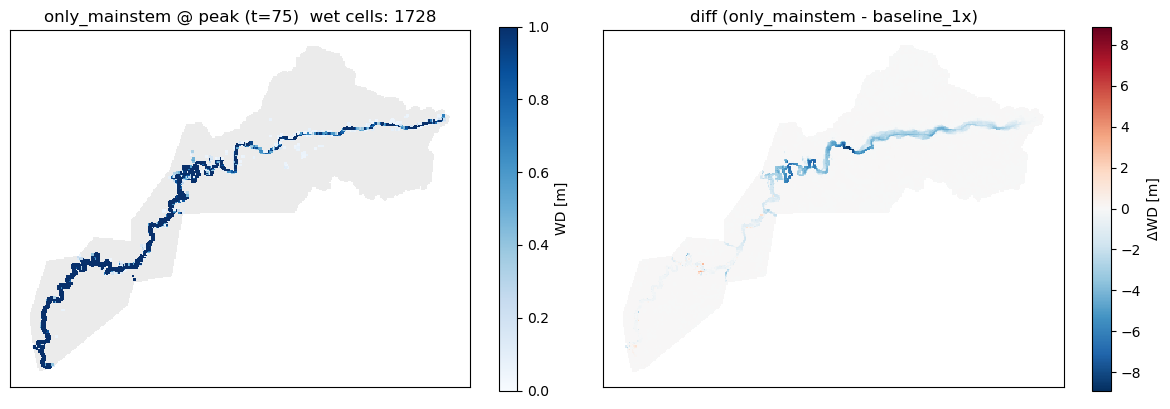
\includegraphics[width=0.8\textwidth]{only_main_20sim.png}
    \caption{Twenty-simulation model, only the main stem active: correctly
      timed ($+1$~h) and reasonably sized ($+11.5\%$ peak error), a sharp
      improvement on the four-simulation model's $-58.2\%$ under-prediction and
      $-10$~h timing failure on the same scenario
      (RMSE~$=0.124$~m, CSI@0.05~$=0.817$, Table~\ref{tab:twentysim-blockbc}).}
    \label{fig:app-e-twentysim-onlymainstem}
\end{figure}

\begin{figure}[H]
    \centering
    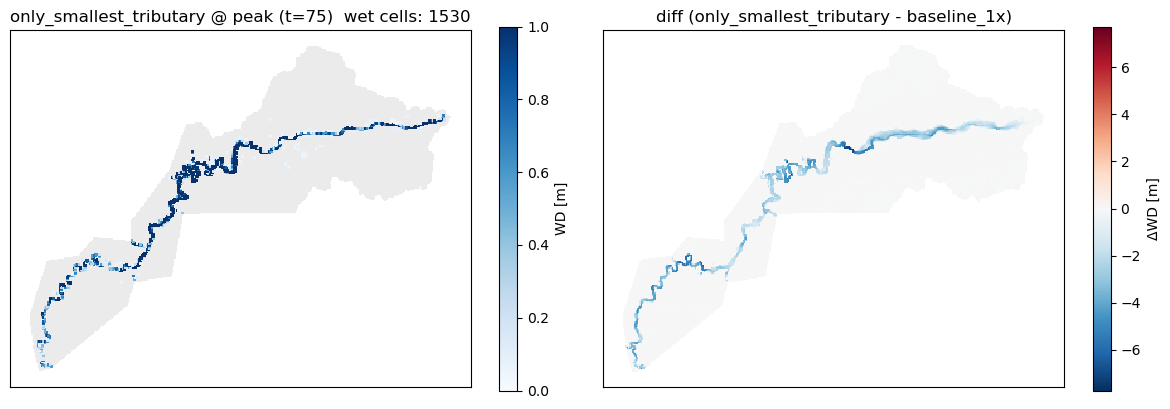
\includegraphics[width=0.8\textwidth]{only_trib_20sim.png}
    \caption{Twenty-simulation model, only the smallest tributary active: peak
      error falls from $+481.9\%$ (four-simulation model) to $+279.6\%$, a real
      improvement but still the largest error in the table
      (RMSE~$=0.154$~m, CSI@0.05~$=0.624$, Table~\ref{tab:twentysim-blockbc}).}
    \label{fig:app-e-twentysim-onlysmallesttrib}
\end{figure}


\section{Per-Location Sensitivity(Zeroed/Doubled)}
\label{app:nonuniform_ladder}

This section supplements the leave-one-out ladder tables.
Bars show the model's response ($|\Delta\text{WDsum@peak}|$, \%); the overlaid
line shows each location's actual volumetric contribution to the flood.
A bar that tracks the line indicates the model
weights that location's forcing roughly in proportion to its real hydrological
contribution.

\begin{figure}[H]
    \centering
    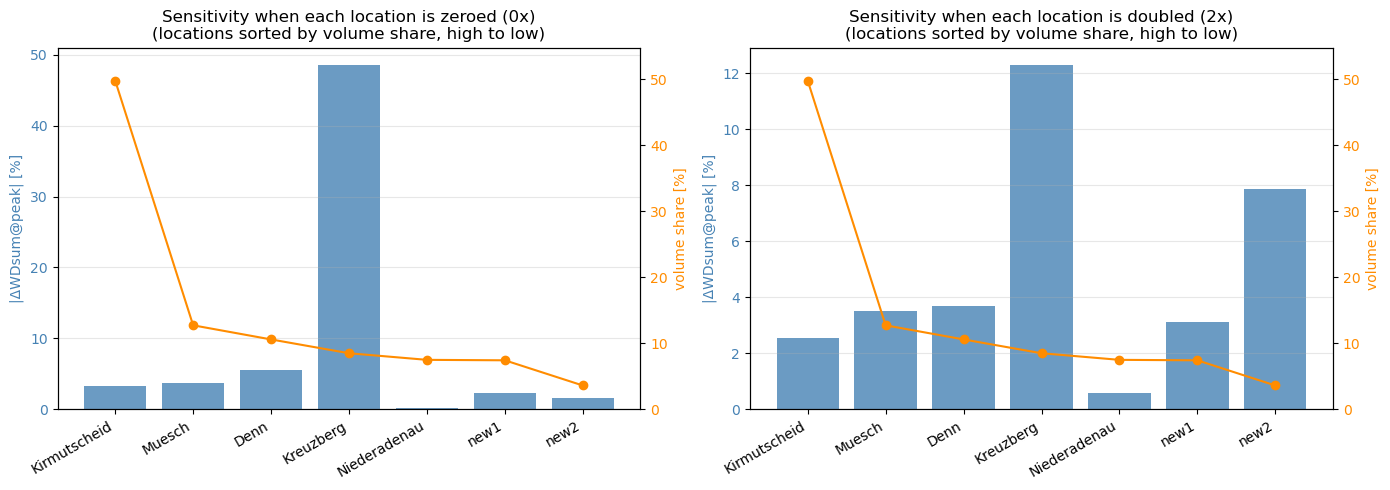
\includegraphics[width=1\textwidth]{sensitivity_perlocation_4sim.png}
    \caption{Four-simulation model: sensitivity when each of the seven
      locations is zeroed (left) or doubled (right).}
    \label{fig:app-e-ladder-foursim}
\end{figure}

\begin{figure}[H]
    \centering
    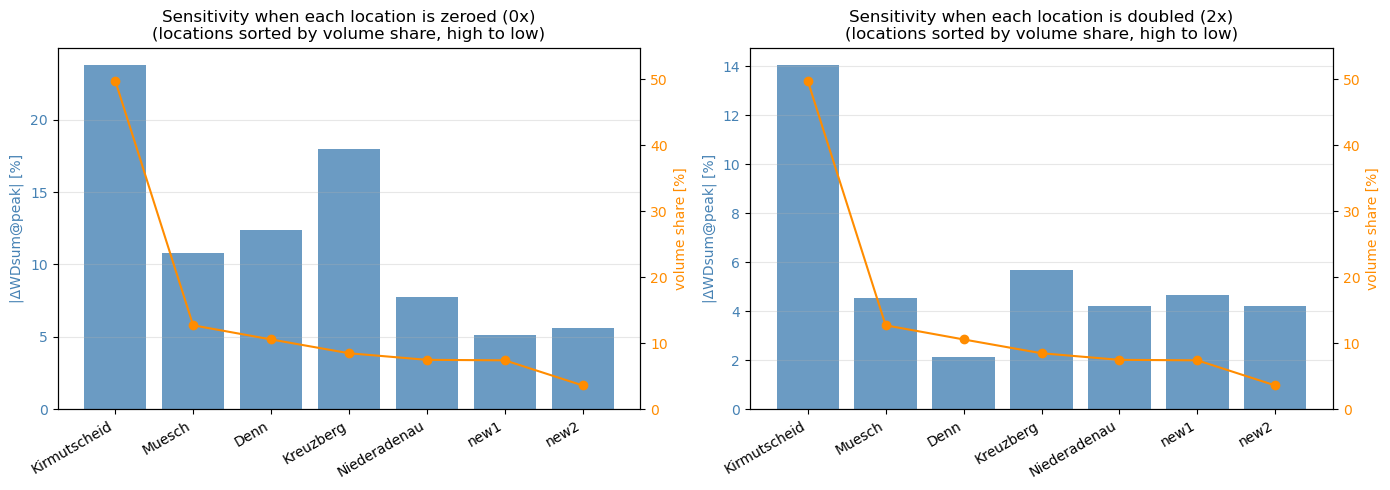
\includegraphics[width=1\textwidth]{sensitivity_perlocation_20sim.png}
    \caption{Twenty-simulation model: same test as
      Figure~\ref{fig:app-e-ladder-foursim}. }
    \label{fig:app-e-ladder-twentysim}
\end{figure}



\chapter{Full-Rollout Evidence for the Reference Models}
\label{app:main_rollouts}

This appendix collects ground-truth-vs-prediction rollout figures for the three
reference models that anchor the main results progression
(Sections~\ref{sec:res_single_sim}, \ref{sec:res_four_sim},
\ref{sec:res_twenty_sim}): the single-, four-, and twenty-simulation models, each
on the held-out $1\times$ event, at the finest mesh scale.

\section{Single-Simulation Model}
\label{app:rollout_singlesim}

\begin{figure}[H]
    \centering
    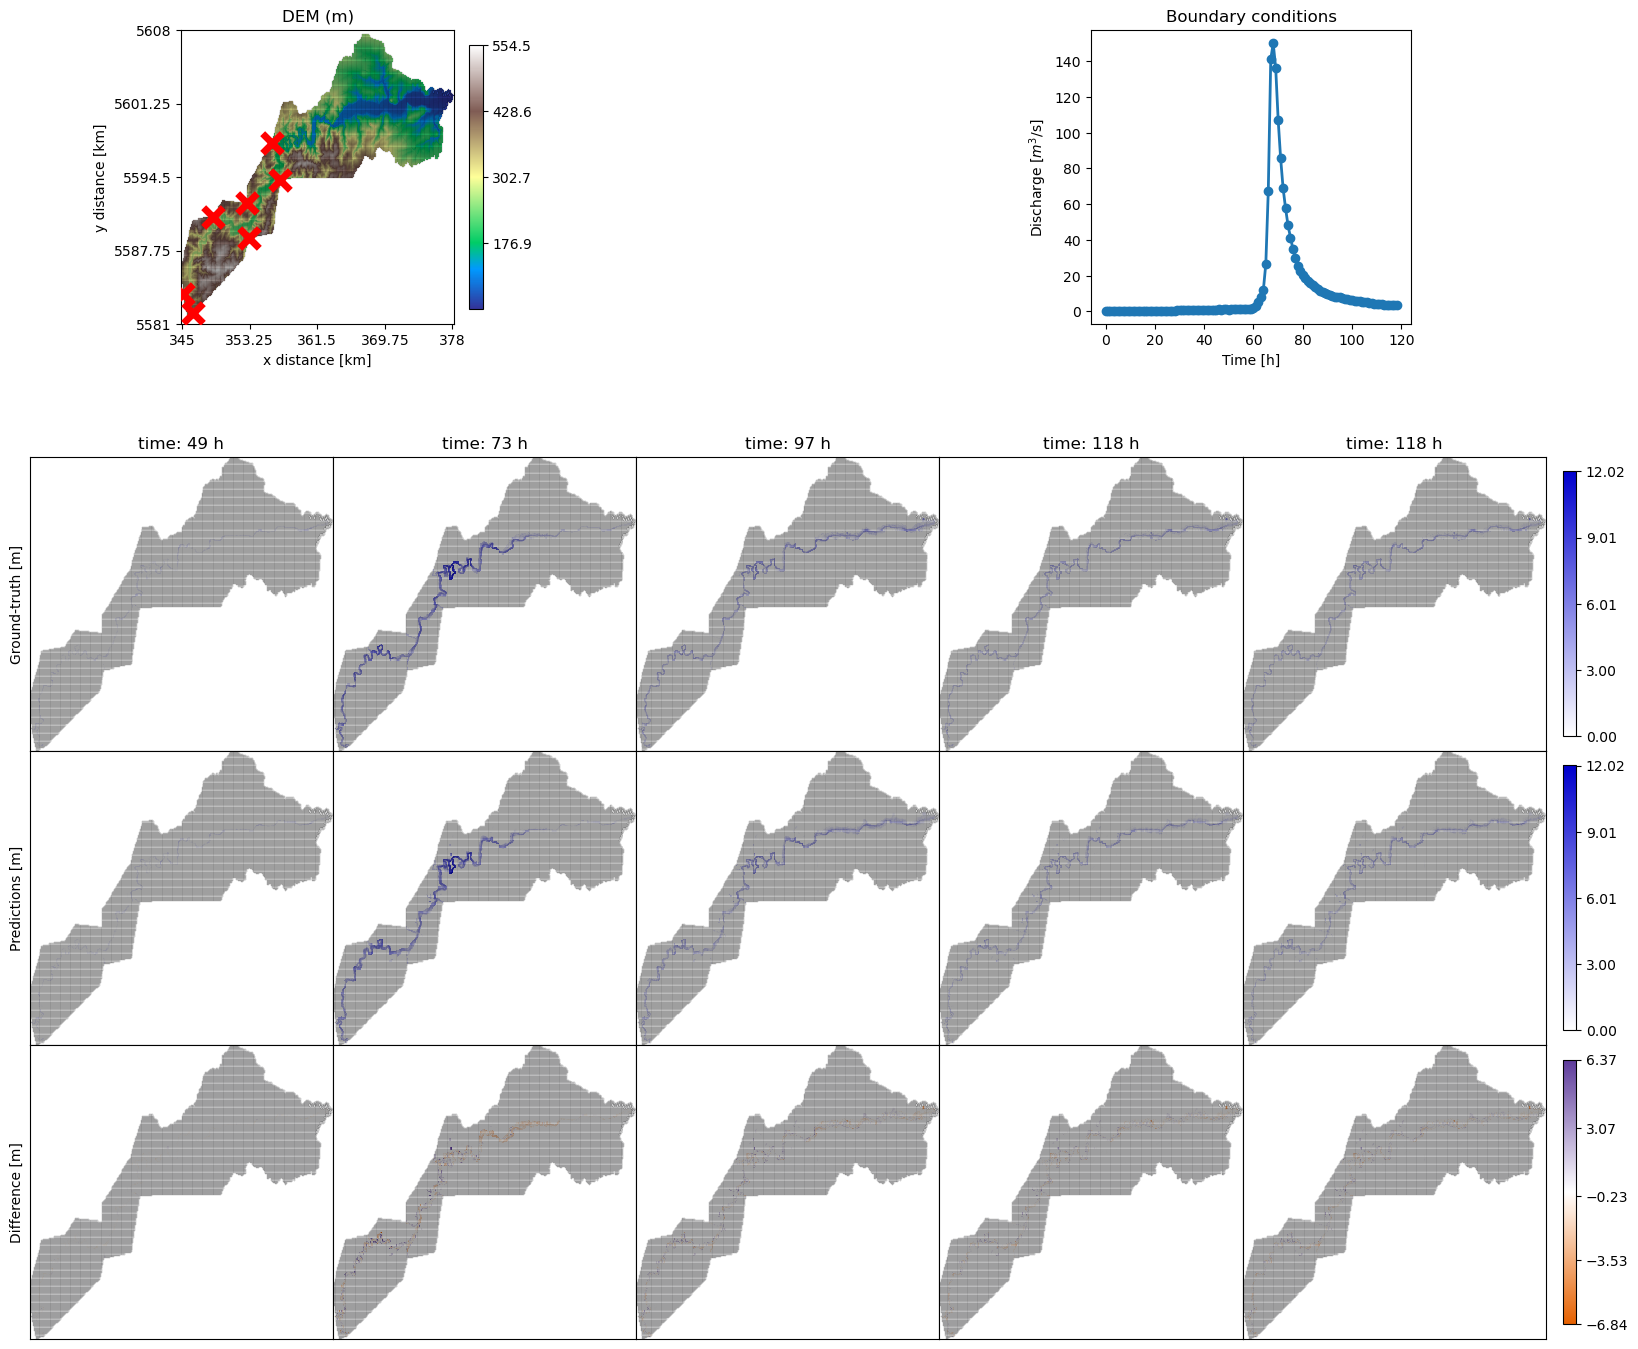
\includegraphics[width=0.95\textwidth]{4sim_fullrollout.png}
    \caption{Model trained with 1 simulation, tested on the training case study. RMSE~$=0.158$~m, CSI@0.05~$=0.775$,
CSI@0.30~$=0.832$.}
    \label{fig:bcaug_fullroll}
\end{figure}


\section{Four-Simulation Model}
\label{app:rollout_foursim}

\begin{figure}[H]
    \centering
    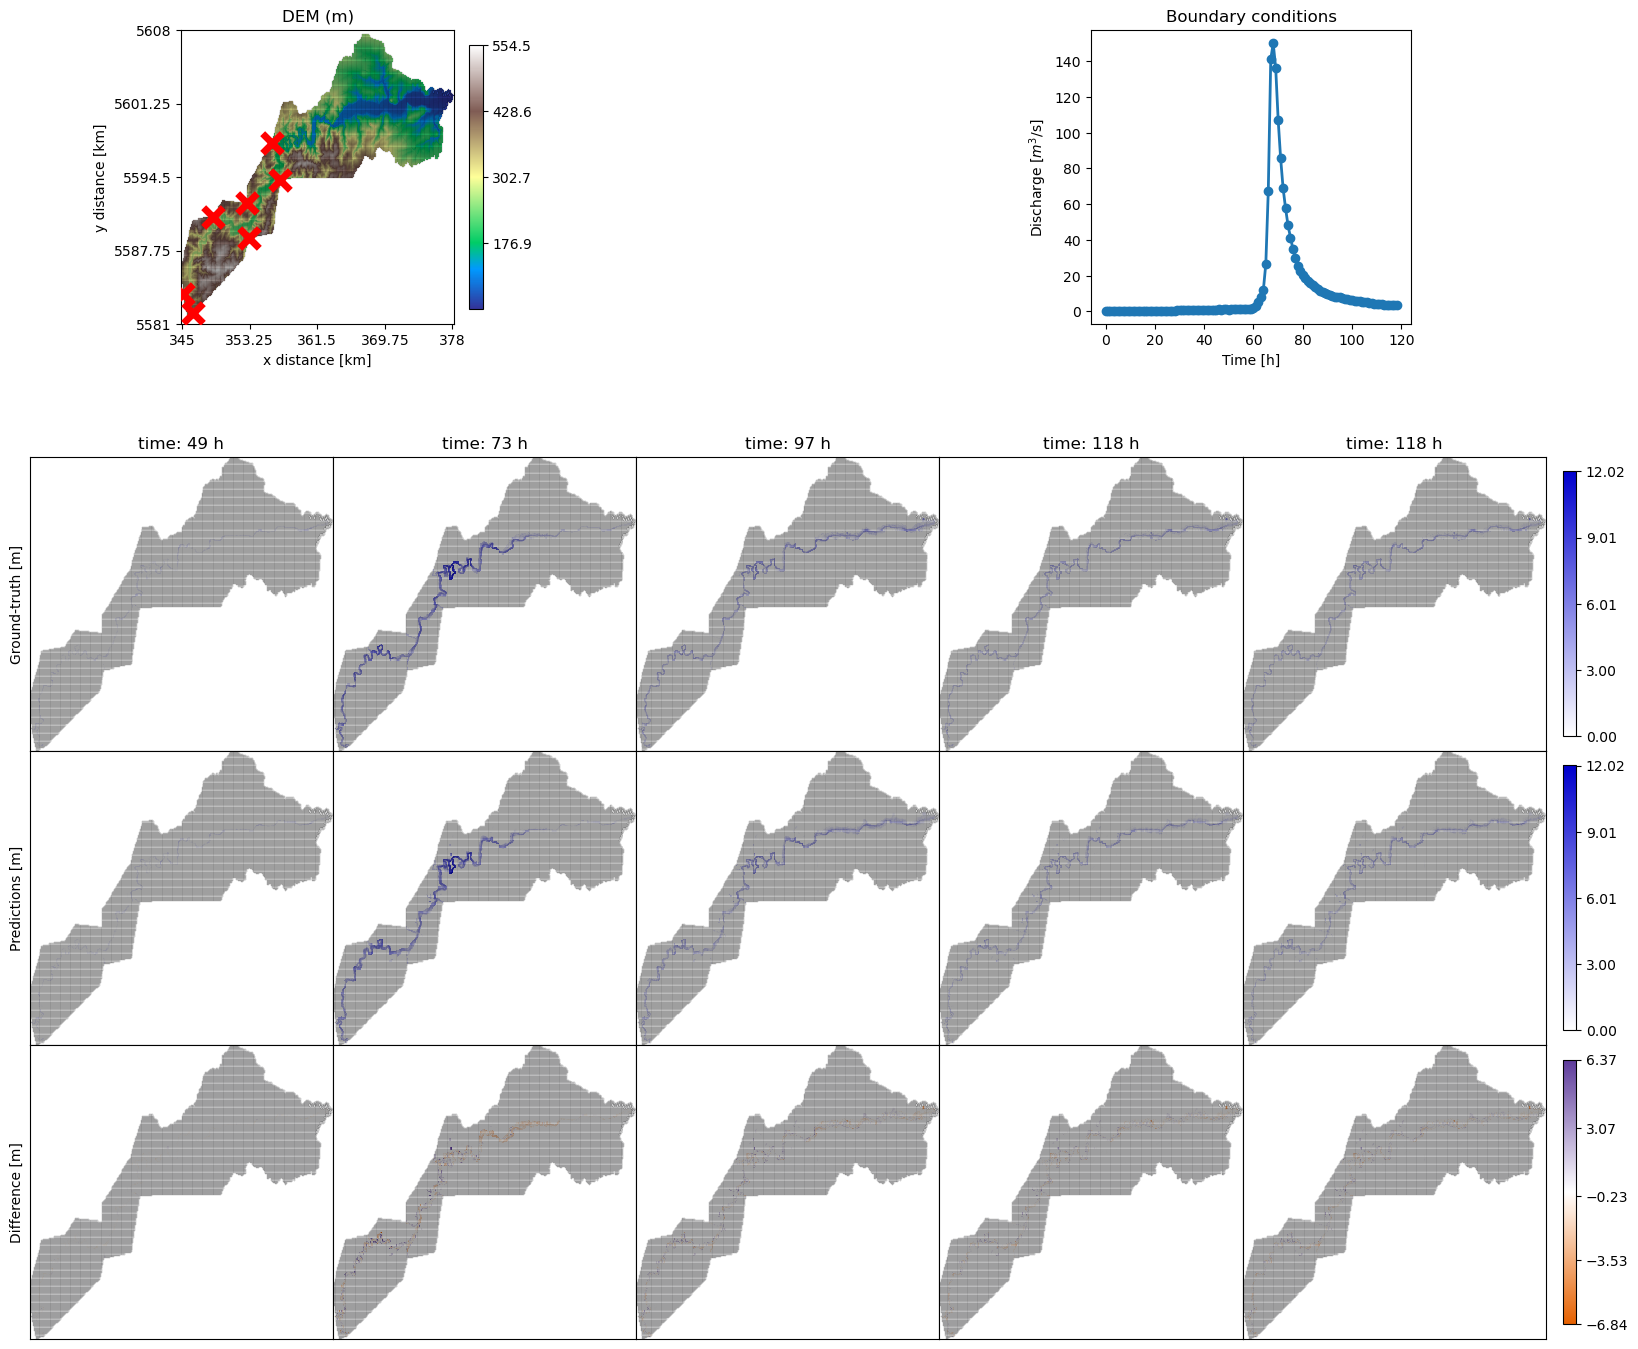
\includegraphics[width=0.95\textwidth]{4sim_fullrollout.png}
    \caption{Model trained with 4 simulations, tested on the held-out 1x case study. RMSE = 0.130 m, CSI@0.05 = 0.799, CSI@0.30 =
0.852.}
    \label{fig:bcaug_fullroll}
\end{figure}

\section{Twenty-Simulation Model}
\label{app:rollout_twentysim}

\begin{figure}[H]
    \centering
    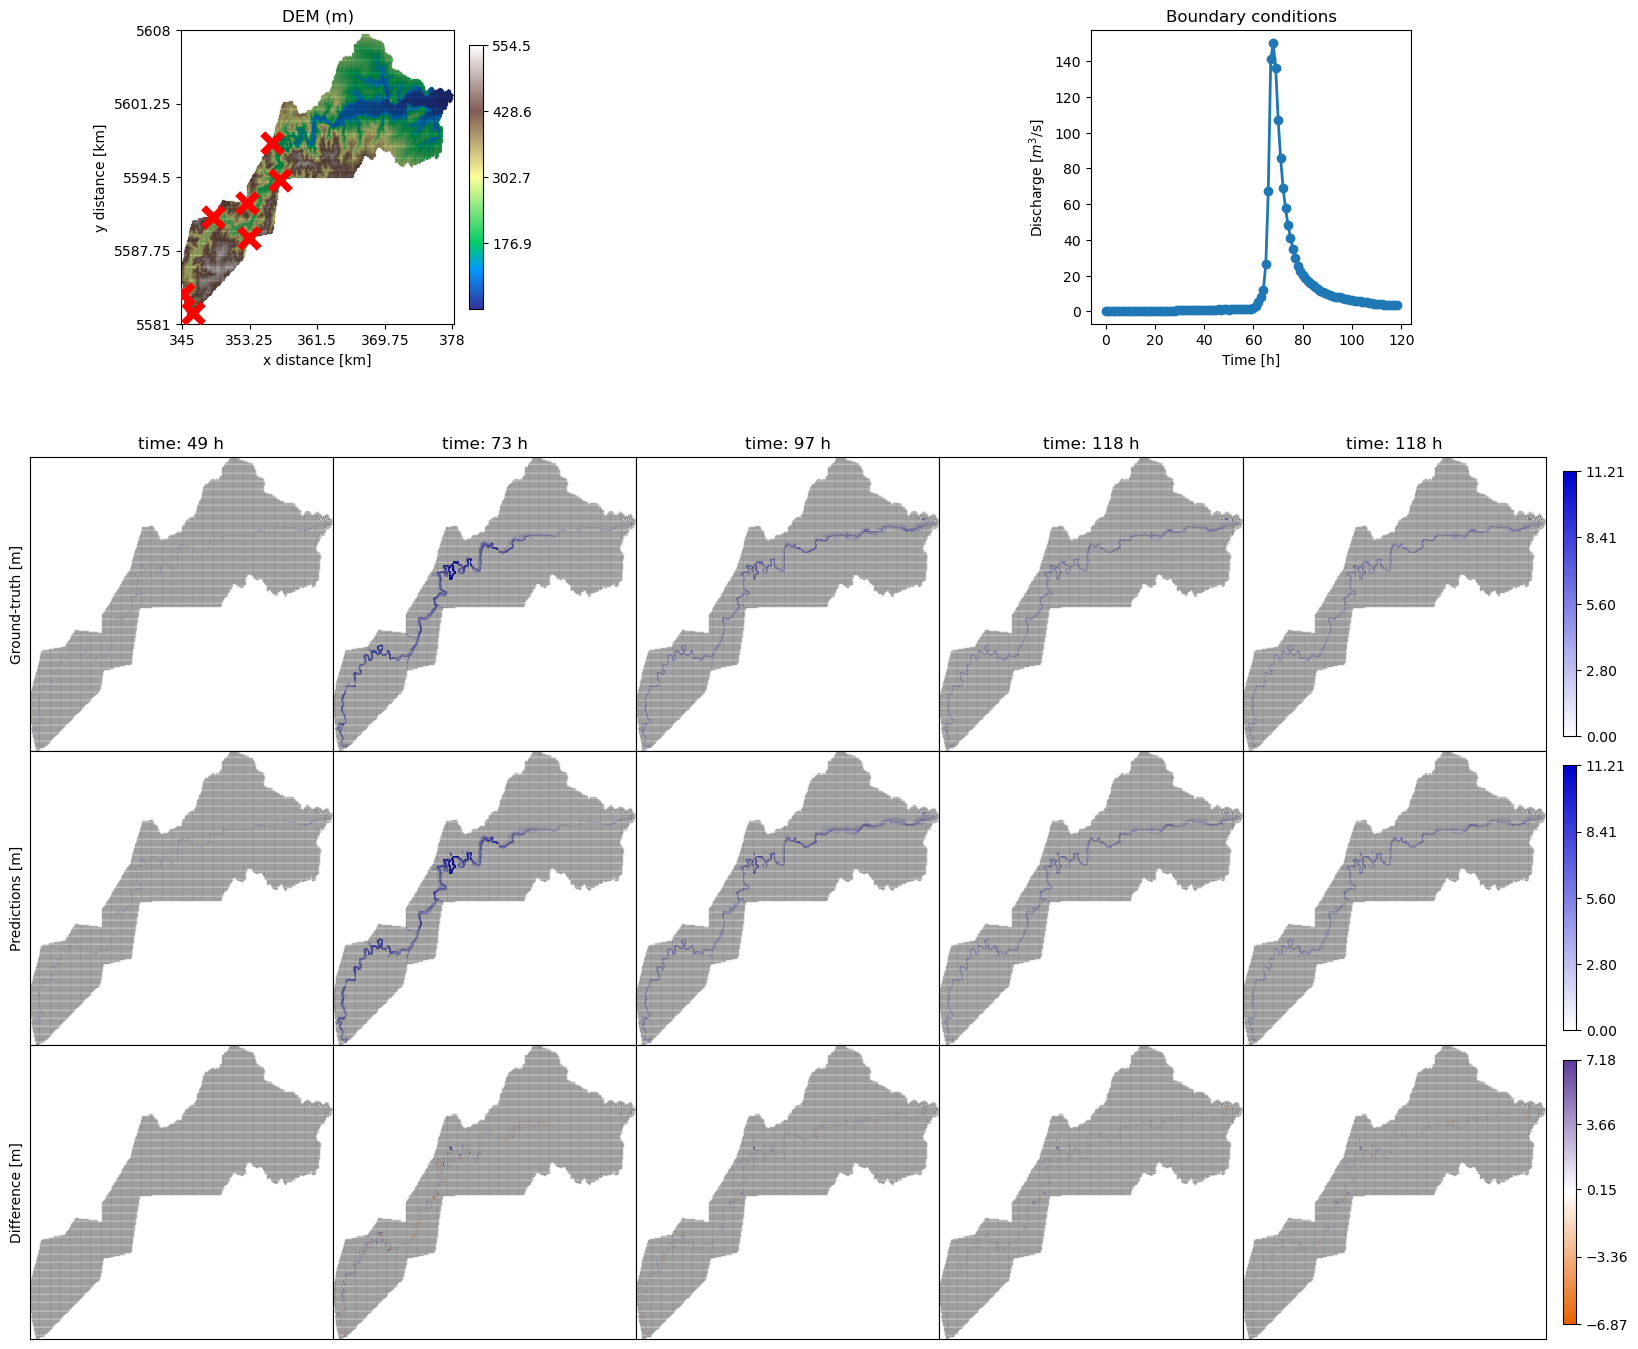
\includegraphics[width=0.95\textwidth]{bc_augum_fullrollout.png}
    \caption{Model trained with 20 simulations, tested on the held-out 1x case study. RMSE =
0.101 m, CSI@0.05 = 0.853, CSI@0.30 = 0.899.}
    \label{fig:bcaug_fullroll}
\end{figure}

\chapter{AI Use Disclosure Statement}

Three distint use of generative AI shaped the production of this thesis.

Already drafted paragraphs were passed through an AI tool for tightening, tone consistency, and grammar checks.

Python code for the analysis and visualisation pipelines was written, debugged, and improved with AI assistance.

Bibliographic entries were cross-checked against their original published sources and
flagged if they needed to be verified more thoroughly by the author.

None of this removes the author's responsibility for what appears in the final
document: every line of AI-touched code, every corrected or replaced citation, and
every reworded passage was checked by hand before being kept. The experiments, results,
and conclusions drawn from them are the author's own work throughout.

\end{document}